\documentclass[twoside]{book}

% Packages required by doxygen
\usepackage{fixltx2e}
\usepackage{calc}
\usepackage{doxygen}
\usepackage{graphicx}
\usepackage[utf8]{inputenc}
\usepackage{makeidx}
\usepackage{multicol}
\usepackage{multirow}
\PassOptionsToPackage{warn}{textcomp}
\usepackage{textcomp}
\usepackage[nointegrals]{wasysym}
\usepackage[table]{xcolor}

% Font selection
\usepackage[T1]{fontenc}
\usepackage{mathptmx}
\usepackage[scaled=.90]{helvet}
\usepackage{courier}
\usepackage{amssymb}
\usepackage{sectsty}
\renewcommand{\familydefault}{\sfdefault}
\allsectionsfont{%
  \fontseries{bc}\selectfont%
  \color{darkgray}%
}
\renewcommand{\DoxyLabelFont}{%
  \fontseries{bc}\selectfont%
  \color{darkgray}%
}
\newcommand{\+}{\discretionary{\mbox{\scriptsize$\hookleftarrow$}}{}{}}

% Page & text layout
\usepackage{geometry}
\geometry{%
  a4paper,%
  top=2.5cm,%
  bottom=2.5cm,%
  left=2.5cm,%
  right=2.5cm%
}
\tolerance=750
\hfuzz=15pt
\hbadness=750
\setlength{\emergencystretch}{15pt}
\setlength{\parindent}{0cm}
\setlength{\parskip}{0.2cm}
\makeatletter
\renewcommand{\paragraph}{%
  \@startsection{paragraph}{4}{0ex}{-1.0ex}{1.0ex}{%
    \normalfont\normalsize\bfseries\SS@parafont%
  }%
}
\renewcommand{\subparagraph}{%
  \@startsection{subparagraph}{5}{0ex}{-1.0ex}{1.0ex}{%
    \normalfont\normalsize\bfseries\SS@subparafont%
  }%
}
\makeatother

% Headers & footers
\usepackage{fancyhdr}
\pagestyle{fancyplain}
\fancyhead[LE]{\fancyplain{}{\bfseries\thepage}}
\fancyhead[CE]{\fancyplain{}{}}
\fancyhead[RE]{\fancyplain{}{\bfseries\leftmark}}
\fancyhead[LO]{\fancyplain{}{\bfseries\rightmark}}
\fancyhead[CO]{\fancyplain{}{}}
\fancyhead[RO]{\fancyplain{}{\bfseries\thepage}}
\fancyfoot[LE]{\fancyplain{}{}}
\fancyfoot[CE]{\fancyplain{}{}}
\fancyfoot[RE]{\fancyplain{}{\bfseries\scriptsize Generated on Sun Feb 1 2015 18\+:56\+:00 for Scaffolding by Doxygen }}
\fancyfoot[LO]{\fancyplain{}{\bfseries\scriptsize Generated on Sun Feb 1 2015 18\+:56\+:00 for Scaffolding by Doxygen }}
\fancyfoot[CO]{\fancyplain{}{}}
\fancyfoot[RO]{\fancyplain{}{}}
\renewcommand{\footrulewidth}{0.4pt}
\renewcommand{\chaptermark}[1]{%
  \markboth{#1}{}%
}
\renewcommand{\sectionmark}[1]{%
  \markright{\thesection\ #1}%
}

% Indices & bibliography
\usepackage{natbib}
\usepackage[titles]{tocloft}
\setcounter{tocdepth}{3}
\setcounter{secnumdepth}{5}
\makeindex

% Hyperlinks (required, but should be loaded last)
\usepackage{ifpdf}
\ifpdf
  \usepackage[pdftex,pagebackref=true]{hyperref}
\else
  \usepackage[ps2pdf,pagebackref=true]{hyperref}
\fi
\hypersetup{%
  colorlinks=true,%
  linkcolor=blue,%
  citecolor=blue,%
  unicode%
}

% Custom commands
\newcommand{\clearemptydoublepage}{%
  \newpage{\pagestyle{empty}\cleardoublepage}%
}


%===== C O N T E N T S =====

\begin{document}

% Titlepage & ToC
\hypersetup{pageanchor=false,
             bookmarks=true,
             bookmarksnumbered=true,
             pdfencoding=unicode
            }
\pagenumbering{roman}
\begin{titlepage}
\vspace*{7cm}
\begin{center}%
{\Large Scaffolding \\[1ex]\large 1.\+5 }\\
\vspace*{1cm}
{\large Generated by Doxygen 1.8.8}\\
\vspace*{0.5cm}
{\small Sun Feb 1 2015 18:56:00}\\
\end{center}
\end{titlepage}
\clearemptydoublepage
\tableofcontents
\clearemptydoublepage
\pagenumbering{arabic}
\hypersetup{pageanchor=true}

%--- Begin generated contents ---
\chapter{Namespace Index}
\section{Packages}
Here are the packages with brief descriptions (if available)\-:\begin{DoxyCompactList}
\item\contentsline{section}{\hyperlink{namespace_scaffolding}{Scaffolding} }{\pageref{namespace_scaffolding}}{}
\end{DoxyCompactList}

\chapter{Hierarchical Index}
\section{Class Hierarchy}
This inheritance list is sorted roughly, but not completely, alphabetically\-:\begin{DoxyCompactList}
\item \contentsline{section}{Scaffolding.\-Input\-Tracker}{\pageref{class_scaffolding_1_1_input_tracker}}{}
\item Mono\-Behaviour\begin{DoxyCompactList}
\item \contentsline{section}{Scaffolding.\-Abstract\-Input}{\pageref{class_scaffolding_1_1_abstract_input}}{}
\begin{DoxyCompactList}
\item \contentsline{section}{Scaffolding.\-Drag\-Input}{\pageref{class_scaffolding_1_1_drag_input}}{}
\begin{DoxyCompactList}
\item \contentsline{section}{Scaffolding.\-Drag\-This\-Input}{\pageref{class_scaffolding_1_1_drag_this_input}}{}
\end{DoxyCompactList}
\item \contentsline{section}{Scaffolding.\-Pinch\-Input}{\pageref{class_scaffolding_1_1_pinch_input}}{}
\begin{DoxyCompactList}
\item \contentsline{section}{Scaffolding.\-Pinch\-This\-Input}{\pageref{class_scaffolding_1_1_pinch_this_input}}{}
\end{DoxyCompactList}
\item \contentsline{section}{Scaffolding.\-Rotate\-Input}{\pageref{class_scaffolding_1_1_rotate_input}}{}
\begin{DoxyCompactList}
\item \contentsline{section}{Scaffolding.\-Rotate\-This\-Input}{\pageref{class_scaffolding_1_1_rotate_this_input}}{}
\end{DoxyCompactList}
\item \contentsline{section}{Scaffolding.\-Scaffolding\-Button}{\pageref{class_scaffolding_1_1_scaffolding_button}}{}
\item \contentsline{section}{Scaffolding.\-Swipe\-Input}{\pageref{class_scaffolding_1_1_swipe_input}}{}
\end{DoxyCompactList}
\item \contentsline{section}{Scaffolding.\-Abstract\-View}{\pageref{class_scaffolding_1_1_abstract_view}}{}
\item \contentsline{section}{Scaffolding.\-Input\-Manager}{\pageref{class_scaffolding_1_1_input_manager}}{}
\item \contentsline{section}{Scaffolding.\-Position\-Item}{\pageref{class_scaffolding_1_1_position_item}}{}
\item \contentsline{section}{Scaffolding.\-View\-Manager}{\pageref{class_scaffolding_1_1_view_manager}}{}
\end{DoxyCompactList}
\item \contentsline{section}{Scaffolding.\-Scaffolding\-Config}{\pageref{class_scaffolding_1_1_scaffolding_config}}{}
\item \contentsline{section}{Scaffolding.\-S\-Object}{\pageref{class_scaffolding_1_1_s_object}}{}
\end{DoxyCompactList}

\chapter{Class Index}
\section{Class List}
Here are the classes, structs, unions and interfaces with brief descriptions\-:\begin{DoxyCompactList}
\item\contentsline{section}{\hyperlink{class_scaffolding_1_1_abstract_input}{Scaffolding.\-Abstract\-Input} \\*Abstract input is responsible for all inputs responding to a touch or input from \hyperlink{class_scaffolding_1_1_input_manager}{Input\-Manager}. }{\pageref{class_scaffolding_1_1_abstract_input}}{}
\item\contentsline{section}{\hyperlink{class_scaffolding_1_1_abstract_view}{Scaffolding.\-Abstract\-View} \\*Abstract view. The base class for any view you wish to create, whether it is a Screen or Overlay. }{\pageref{class_scaffolding_1_1_abstract_view}}{}
\item\contentsline{section}{\hyperlink{class_scaffolding_1_1_drag_input}{Scaffolding.\-Drag\-Input} \\*Drag input is a quick dragging solution using \hyperlink{class_scaffolding_1_1_abstract_input}{Abstract\-Input}. }{\pageref{class_scaffolding_1_1_drag_input}}{}
\item\contentsline{section}{\hyperlink{class_scaffolding_1_1_drag_this_input}{Scaffolding.\-Drag\-This\-Input} \\*\hyperlink{class_scaffolding_1_1_drag_this_input}{Drag\-This\-Input} attaches to a gameobject as a quick solution to get something draggable. Extends \hyperlink{class_scaffolding_1_1_abstract_input}{Abstract\-Input} so falls under the same rules as other inputs in regards to views. E.\-g colliders get disabled during On\-Show\-Start and On\-Hide\-Start phases. }{\pageref{class_scaffolding_1_1_drag_this_input}}{}
\item\contentsline{section}{\hyperlink{class_scaffolding_1_1_input_manager}{Scaffolding.\-Input\-Manager} \\*Scaffoldings \hyperlink{class_scaffolding_1_1_input_manager}{Input\-Manager} is a multitouch input manager that looks after all the inputs used within scaffoldings \hyperlink{class_scaffolding_1_1_abstract_input}{Abstract\-Input} class. \hyperlink{namespace_scaffolding}{Scaffolding} is multitouch from the core and built upon the idea that you should be able to place your whole hand on the screen and still use buttons. }{\pageref{class_scaffolding_1_1_input_manager}}{}
\item\contentsline{section}{\hyperlink{class_scaffolding_1_1_input_tracker}{Scaffolding.\-Input\-Tracker} \\*Input tracker, tracks every finger or mouse press that happens within Scaffoldings views. }{\pageref{class_scaffolding_1_1_input_tracker}}{}
\item\contentsline{section}{\hyperlink{class_scaffolding_1_1_pinch_input}{Scaffolding.\-Pinch\-Input} \\*Pinch input is largely a touch input based class. It replicates the pinch gesture, and dispatches a callback while pinching. }{\pageref{class_scaffolding_1_1_pinch_input}}{}
\item\contentsline{section}{\hyperlink{class_scaffolding_1_1_pinch_this_input}{Scaffolding.\-Pinch\-This\-Input} \\*\hyperlink{class_scaffolding_1_1_pinch_this_input}{Pinch\-This\-Input} attaches to a gameobject as a quick solution to get something to respond to the pinch gesture. Extends \hyperlink{class_scaffolding_1_1_abstract_input}{Abstract\-Input} so falls under the same rules as other inputs in regards to views. E.\-g colliders get disabled during On\-Show\-Start and On\-Hide\-Start phases }{\pageref{class_scaffolding_1_1_pinch_this_input}}{}
\item\contentsline{section}{\hyperlink{class_scaffolding_1_1_position_item}{Scaffolding.\-Position\-Item} \\*Positions the transform relative to a camera. Only works with Orthographic cameras currently. }{\pageref{class_scaffolding_1_1_position_item}}{}
\item\contentsline{section}{\hyperlink{class_scaffolding_1_1_rotate_input}{Scaffolding.\-Rotate\-Input} \\*Rotate input is largely a touch input based class. It replicates the rotate gesture, and dispatches a callback while rotating. }{\pageref{class_scaffolding_1_1_rotate_input}}{}
\item\contentsline{section}{\hyperlink{class_scaffolding_1_1_rotate_this_input}{Scaffolding.\-Rotate\-This\-Input} \\*\hyperlink{class_scaffolding_1_1_rotate_this_input}{Rotate\-This\-Input} attaches to a gameobject as a quick solution to get something to respond to the rotate gesture. Extends \hyperlink{class_scaffolding_1_1_abstract_input}{Abstract\-Input} so falls under the same rules as other inputs in regards to views. E.\-g colliders get disabled during On\-Show\-Start and On\-Hide\-Start phases }{\pageref{class_scaffolding_1_1_rotate_this_input}}{}
\item\contentsline{section}{\hyperlink{class_scaffolding_1_1_scaffolding_button}{Scaffolding.\-Scaffolding\-Button} \\*The button class associated with the \hyperlink{namespace_scaffolding}{Scaffolding} default buttons }{\pageref{class_scaffolding_1_1_scaffolding_button}}{}
\item\contentsline{section}{\hyperlink{class_scaffolding_1_1_scaffolding_config}{Scaffolding.\-Scaffolding\-Config} }{\pageref{class_scaffolding_1_1_scaffolding_config}}{}
\item\contentsline{section}{\hyperlink{class_scaffolding_1_1_s_object}{Scaffolding.\-S\-Object} \\*Value object. Used for passing data between views. Pack any data you require into this, and On\-Show\-Start can retrieve it. }{\pageref{class_scaffolding_1_1_s_object}}{}
\item\contentsline{section}{\hyperlink{class_scaffolding_1_1_swipe_input}{Scaffolding.\-Swipe\-Input} \\*Swipe input replicates the swipe gesture and dispatches a callback for a chosen swipe direction. }{\pageref{class_scaffolding_1_1_swipe_input}}{}
\item\contentsline{section}{\hyperlink{class_scaffolding_1_1_view_manager}{Scaffolding.\-View\-Manager} }{\pageref{class_scaffolding_1_1_view_manager}}{}
\end{DoxyCompactList}

\chapter{Namespace Documentation}
\hypertarget{namespace_scaffolding}{\section{Package Scaffolding}
\label{namespace_scaffolding}\index{Scaffolding@{Scaffolding}}
}
\subsection*{Classes}
\begin{DoxyCompactItemize}
\item 
class \hyperlink{class_scaffolding_1_1_scaffolding_config}{Scaffolding\-Config}
\item 
class {\bfseries Scaffolding\-Extensions}
\item 
class \hyperlink{class_scaffolding_1_1_s_object}{S\-Object}
\begin{DoxyCompactList}\small\item\em Value object. Used for passing data between views. Pack any data you require into this, and On\-Show\-Start can retrieve it. \end{DoxyCompactList}\item 
class \hyperlink{class_scaffolding_1_1_abstract_input}{Abstract\-Input}
\begin{DoxyCompactList}\small\item\em Abstract input is responsible for all inputs responding to a touch or input from \hyperlink{class_scaffolding_1_1_input_manager}{Input\-Manager}. \end{DoxyCompactList}\item 
class \hyperlink{class_scaffolding_1_1_input_manager}{Input\-Manager}
\begin{DoxyCompactList}\small\item\em Scaffoldings \hyperlink{class_scaffolding_1_1_input_manager}{Input\-Manager} is a multitouch input manager that looks after all the inputs used within scaffoldings \hyperlink{class_scaffolding_1_1_abstract_input}{Abstract\-Input} class. \hyperlink{namespace_scaffolding}{Scaffolding} is multitouch from the core and built upon the idea that you should be able to place your whole hand on the screen and still use buttons. \end{DoxyCompactList}\item 
class \hyperlink{class_scaffolding_1_1_input_tracker}{Input\-Tracker}
\begin{DoxyCompactList}\small\item\em Input tracker, tracks every finger or mouse press that happens within Scaffoldings views. \end{DoxyCompactList}\item 
class \hyperlink{class_scaffolding_1_1_drag_input}{Drag\-Input}
\begin{DoxyCompactList}\small\item\em Drag input is a quick dragging solution using \hyperlink{class_scaffolding_1_1_abstract_input}{Abstract\-Input}. \end{DoxyCompactList}\item 
class \hyperlink{class_scaffolding_1_1_drag_this_input}{Drag\-This\-Input}
\begin{DoxyCompactList}\small\item\em \hyperlink{class_scaffolding_1_1_drag_this_input}{Drag\-This\-Input} attaches to a gameobject as a quick solution to get something draggable. Extends \hyperlink{class_scaffolding_1_1_abstract_input}{Abstract\-Input} so falls under the same rules as other inputs in regards to views. E.\-g colliders get disabled during On\-Show\-Start and On\-Hide\-Start phases. \end{DoxyCompactList}\item 
class \hyperlink{class_scaffolding_1_1_pinch_input}{Pinch\-Input}
\begin{DoxyCompactList}\small\item\em Pinch input is largely a touch input based class. It replicates the pinch gesture, and dispatches a callback while pinching. \end{DoxyCompactList}\item 
class \hyperlink{class_scaffolding_1_1_pinch_this_input}{Pinch\-This\-Input}
\begin{DoxyCompactList}\small\item\em \hyperlink{class_scaffolding_1_1_pinch_this_input}{Pinch\-This\-Input} attaches to a gameobject as a quick solution to get something to respond to the pinch gesture. Extends \hyperlink{class_scaffolding_1_1_abstract_input}{Abstract\-Input} so falls under the same rules as other inputs in regards to views. E.\-g colliders get disabled during On\-Show\-Start and On\-Hide\-Start phases. \end{DoxyCompactList}\item 
class \hyperlink{class_scaffolding_1_1_position_item}{Position\-Item}
\begin{DoxyCompactList}\small\item\em Positions the transform relative to a camera. Only works with Orthographic cameras currently. \end{DoxyCompactList}\item 
class \hyperlink{class_scaffolding_1_1_rotate_input}{Rotate\-Input}
\begin{DoxyCompactList}\small\item\em Rotate input is largely a touch input based class. It replicates the rotate gesture, and dispatches a callback while rotating. \end{DoxyCompactList}\item 
class \hyperlink{class_scaffolding_1_1_rotate_this_input}{Rotate\-This\-Input}
\begin{DoxyCompactList}\small\item\em \hyperlink{class_scaffolding_1_1_rotate_this_input}{Rotate\-This\-Input} attaches to a gameobject as a quick solution to get something to respond to the rotate gesture. Extends \hyperlink{class_scaffolding_1_1_abstract_input}{Abstract\-Input} so falls under the same rules as other inputs in regards to views. E.\-g colliders get disabled during On\-Show\-Start and On\-Hide\-Start phases. \end{DoxyCompactList}\item 
class \hyperlink{class_scaffolding_1_1_scaffolding_button}{Scaffolding\-Button}
\begin{DoxyCompactList}\small\item\em The button class associated with the \hyperlink{namespace_scaffolding}{Scaffolding} default buttons. \end{DoxyCompactList}\item 
class \hyperlink{class_scaffolding_1_1_swipe_input}{Swipe\-Input}
\begin{DoxyCompactList}\small\item\em Swipe input replicates the swipe gesture and dispatches a callback for a chosen swipe direction. \end{DoxyCompactList}\item 
class \hyperlink{class_scaffolding_1_1_abstract_view}{Abstract\-View}
\begin{DoxyCompactList}\small\item\em Abstract view. The base class for any view you wish to create, whether it is a Screen or Overlay. \end{DoxyCompactList}\item 
class \hyperlink{class_scaffolding_1_1_view_manager}{View\-Manager}
\end{DoxyCompactItemize}
\subsection*{Enumerations}
\begin{DoxyCompactItemize}
\item 
enum {\bfseries Swipe\-Direction} \{ {\bfseries Left}, 
{\bfseries Right}, 
{\bfseries Up}, 
{\bfseries Down}
 \}
\end{DoxyCompactItemize}

\chapter{Class Documentation}
\hypertarget{class_scaffolding_1_1_abstract_button}{\section{Scaffolding.\+Abstract\+Button Class Reference}
\label{class_scaffolding_1_1_abstract_button}\index{Scaffolding.\+Abstract\+Button@{Scaffolding.\+Abstract\+Button}}
}
Inheritance diagram for Scaffolding.\+Abstract\+Button\+:\begin{figure}[H]
\begin{center}
\leavevmode
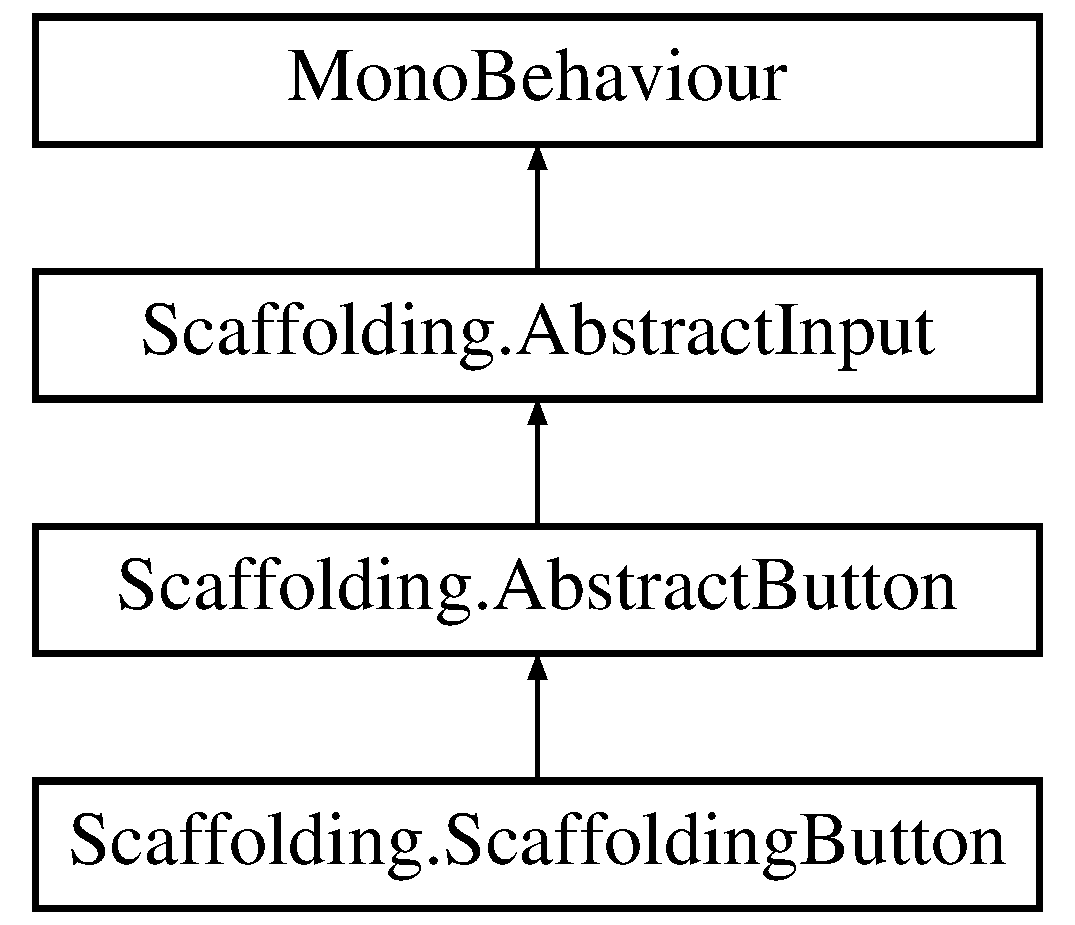
\includegraphics[height=4.000000cm]{class_scaffolding_1_1_abstract_button}
\end{center}
\end{figure}
\subsection*{Public Types}
\begin{DoxyCompactItemize}
\item 
\hypertarget{class_scaffolding_1_1_abstract_button_a8570e566f4323db9e5b65bf214ec5bc4}{enum {\bfseries Button\+Action\+Type} \{ {\bfseries Do\+Nothing}, 
{\bfseries Open}, 
{\bfseries Close}
 \}}\label{class_scaffolding_1_1_abstract_button_a8570e566f4323db9e5b65bf214ec5bc4}

\item 
\hypertarget{class_scaffolding_1_1_abstract_button_ab12f25762012b4eaf00e4a8036cb715b}{enum {\bfseries Button\+State} \{ {\bfseries Up}, 
{\bfseries Down}, 
{\bfseries Inactive}
 \}}\label{class_scaffolding_1_1_abstract_button_ab12f25762012b4eaf00e4a8036cb715b}

\end{DoxyCompactItemize}
\subsection*{Public Member Functions}
\begin{DoxyCompactItemize}
\item 
override void \hyperlink{class_scaffolding_1_1_abstract_button_aa9ef22706bd2af0de02ec86f4d6641d4}{Setup} (\hyperlink{class_scaffolding_1_1_abstract_view}{Abstract\+View} view)
\begin{DoxyCompactList}\small\item\em Run by the view during it's setup phase. \end{DoxyCompactList}\item 
override void \hyperlink{class_scaffolding_1_1_abstract_button_ae8879dc8ec6de80c1c75d7399ebffe90}{Cleanup} ()
\begin{DoxyCompactList}\small\item\em The inputs clean up phase. \end{DoxyCompactList}\item 
\hypertarget{class_scaffolding_1_1_abstract_button_a8ba5b844a0a9af02bb60aefc4a6f8a6f}{virtual void {\bfseries Button\+Pressed} ()}\label{class_scaffolding_1_1_abstract_button_a8ba5b844a0a9af02bb60aefc4a6f8a6f}

\item 
\hypertarget{class_scaffolding_1_1_abstract_button_ae6dddf72812ac62282f3cde509f6b43b}{virtual void {\bfseries Button\+Down} ()}\label{class_scaffolding_1_1_abstract_button_ae6dddf72812ac62282f3cde509f6b43b}

\item 
\hypertarget{class_scaffolding_1_1_abstract_button_a672ed0b6c81579cd2daaa7c0274bcdb0}{void {\bfseries Toggle\+Button\+Inactive} (bool active)}\label{class_scaffolding_1_1_abstract_button_a672ed0b6c81579cd2daaa7c0274bcdb0}

\item 
virtual void \hyperlink{class_scaffolding_1_1_abstract_button_ae18ef32bad19d3fd5159bc825c9a1211}{Change\+State} (Button\+State state)
\begin{DoxyCompactList}\small\item\em Changes the buttons visual state. \end{DoxyCompactList}\item 
void \hyperlink{class_scaffolding_1_1_abstract_button_a8862a2385e9d955cf58a878828ddde05}{Open\+View\+On\+Pressed} (Type target)
\begin{DoxyCompactList}\small\item\em Set the Screen to be opened when the button is pressed. \end{DoxyCompactList}\item 
void \hyperlink{class_scaffolding_1_1_abstract_button_a2580b5e356bcda58ab8f7de52679c211}{Open\+View\+On\+Pressed$<$ T $>$} ()
\begin{DoxyCompactList}\small\item\em Set the Screen to be opened when the button is pressed. \end{DoxyCompactList}\item 
void \hyperlink{class_scaffolding_1_1_abstract_button_acba98947a8987ad65e7ce34114e903cf}{Open\+View\+On\+Pressed} (Type target, Type loading\+View)
\begin{DoxyCompactList}\small\item\em Set the screen to be opened when the button is pressed. Set the loading overlay to be opened first to mask heavy loading. \end{DoxyCompactList}\item 
void \hyperlink{class_scaffolding_1_1_abstract_button_adc646043693b169f9810a6c0bf662007}{Open\+View\+On\+Pressed$<$ T, L $>$} ()
\begin{DoxyCompactList}\small\item\em Set the screen to be opened when the button is pressed. Set the loading overlay to be opened first to mask heavy loading. \end{DoxyCompactList}\item 
void \hyperlink{class_scaffolding_1_1_abstract_button_a1087cf2c11995a65a0432bccdd930fd6}{Open\+Overlay\+On\+Pressed} (Type target\+Overlay)
\begin{DoxyCompactList}\small\item\em Set the overlay to be opened when the button is pressed. \end{DoxyCompactList}\item 
void \hyperlink{class_scaffolding_1_1_abstract_button_a71ab29dc963545c57b57aa9a294f5be1}{Open\+Overlay\+On\+Pressed$<$ T $>$} ()
\begin{DoxyCompactList}\small\item\em Set the overlay to be opened when the button is pressed. \end{DoxyCompactList}\item 
void \hyperlink{class_scaffolding_1_1_abstract_button_abb180405fc64d38655f5be2a935dc71c}{Close\+Overlay\+On\+Pressed} (Type target\+Overlay)
\begin{DoxyCompactList}\small\item\em Set the overlay to be closed when the button is pressed. \end{DoxyCompactList}\item 
void \hyperlink{class_scaffolding_1_1_abstract_button_acf05350651bf38ee6c7928c6c2f35c54}{Close\+Overlay\+On\+Pressed$<$ T $>$} ()
\begin{DoxyCompactList}\small\item\em Set the overlay to be closed when the button is pressed. \end{DoxyCompactList}\item 
void \hyperlink{class_scaffolding_1_1_abstract_button_ae99a36e41eb5d2975137669c44aafe26}{Add\+Button\+Pressed\+Handler} (Action$<$ \hyperlink{class_scaffolding_1_1_abstract_button}{Abstract\+Button} $>$ action)
\begin{DoxyCompactList}\small\item\em Registers the button pressed callback. \end{DoxyCompactList}\item 
void \hyperlink{class_scaffolding_1_1_abstract_button_a797be871a53380fa6aaed1bad0d64002}{Add\+Button\+Pressed\+Handler\+No\+Button} (Action action)
\begin{DoxyCompactList}\small\item\em Registers the button pressed callback.. \end{DoxyCompactList}\item 
void \hyperlink{class_scaffolding_1_1_abstract_button_ac5e452a4c33391900a861e2e0275cc58}{Add\+Button\+Down\+Handler} (Action$<$ \hyperlink{class_scaffolding_1_1_abstract_button}{Abstract\+Button} $>$ action)
\begin{DoxyCompactList}\small\item\em Registers the button down callback. \end{DoxyCompactList}\item 
void \hyperlink{class_scaffolding_1_1_abstract_button_a33bcbcb549fceb9e1f6df0b0fff440aa}{Add\+Button\+Down\+Handler\+No\+Button} (Action action)
\begin{DoxyCompactList}\small\item\em Registers the button down callback. \end{DoxyCompactList}\end{DoxyCompactItemize}
\subsection*{Public Attributes}
\begin{DoxyCompactItemize}
\item 
\hypertarget{class_scaffolding_1_1_abstract_button_a3964c7b7750ae8a2616d1ec95ef2961d}{string {\bfseries target\+View}}\label{class_scaffolding_1_1_abstract_button_a3964c7b7750ae8a2616d1ec95ef2961d}

\item 
\hypertarget{class_scaffolding_1_1_abstract_button_af1415e2079d38ab6514fdba3a29d6a65}{int {\bfseries target\+View\+Index}}\label{class_scaffolding_1_1_abstract_button_af1415e2079d38ab6514fdba3a29d6a65}

\item 
\hypertarget{class_scaffolding_1_1_abstract_button_adf6d52ebbf1d039ff8bc2add1fec61bd}{int {\bfseries target\+View\+Length}}\label{class_scaffolding_1_1_abstract_button_adf6d52ebbf1d039ff8bc2add1fec61bd}

\item 
\hypertarget{class_scaffolding_1_1_abstract_button_a0368194bc658fc41d470caaa4613d6fc}{string {\bfseries input\+Camera}}\label{class_scaffolding_1_1_abstract_button_a0368194bc658fc41d470caaa4613d6fc}

\item 
\hypertarget{class_scaffolding_1_1_abstract_button_ad62400a6c2dd73d00d4323d9e22ad3bf}{int {\bfseries input\+Camera\+Index}}\label{class_scaffolding_1_1_abstract_button_ad62400a6c2dd73d00d4323d9e22ad3bf}

\item 
\hypertarget{class_scaffolding_1_1_abstract_button_a7d1ed91db6beff4dbd8cbca02302f4aa}{int {\bfseries input\+Camera\+Length}}\label{class_scaffolding_1_1_abstract_button_a7d1ed91db6beff4dbd8cbca02302f4aa}

\item 
\hypertarget{class_scaffolding_1_1_abstract_button_afabca95e2175e1dc3000ca60d5593bb7}{string {\bfseries loading\+Overlay}}\label{class_scaffolding_1_1_abstract_button_afabca95e2175e1dc3000ca60d5593bb7}

\item 
\hypertarget{class_scaffolding_1_1_abstract_button_a99eac01e9ba3a61018e5424942fd82e3}{bool {\bfseries open\+As\+Screen} = true}\label{class_scaffolding_1_1_abstract_button_a99eac01e9ba3a61018e5424942fd82e3}

\item 
\hypertarget{class_scaffolding_1_1_abstract_button_ae005c481844dab665e7ad68c7655ef93}{bool {\bfseries disable\+Inputs\+On\+Overlay} = false}\label{class_scaffolding_1_1_abstract_button_ae005c481844dab665e7ad68c7655ef93}

\item 
\hypertarget{class_scaffolding_1_1_abstract_button_aea0592d79dd8b035de641dcdf943f5b6}{bool {\bfseries open\+Loading\+Overlay} = false}\label{class_scaffolding_1_1_abstract_button_aea0592d79dd8b035de641dcdf943f5b6}

\item 
\hypertarget{class_scaffolding_1_1_abstract_button_a51a8f08a8b61d48549750ee0afa3b8c2}{Button\+Action\+Type {\bfseries button\+Action\+Type}}\label{class_scaffolding_1_1_abstract_button_a51a8f08a8b61d48549750ee0afa3b8c2}

\item 
\hypertarget{class_scaffolding_1_1_abstract_button_ab1319d3e572a56ca6f32b034c1e25197}{List$<$ int $>$ {\bfseries selected\+Script\+Index}}\label{class_scaffolding_1_1_abstract_button_ab1319d3e572a56ca6f32b034c1e25197}

\item 
\hypertarget{class_scaffolding_1_1_abstract_button_a84730e9b36659535b38d1c177f87bfa7}{List$<$ int $>$ {\bfseries selected\+Script\+Length}}\label{class_scaffolding_1_1_abstract_button_a84730e9b36659535b38d1c177f87bfa7}

\item 
\hypertarget{class_scaffolding_1_1_abstract_button_aaf2a5387f50d2b7fa3b25a07a54e9330}{List$<$ string $>$ {\bfseries selected\+Script}}\label{class_scaffolding_1_1_abstract_button_aaf2a5387f50d2b7fa3b25a07a54e9330}

\item 
\hypertarget{class_scaffolding_1_1_abstract_button_a5217705c6d3e1eae6465bf019c4cc66e}{List$<$ int $>$ {\bfseries selected\+Method\+Index}}\label{class_scaffolding_1_1_abstract_button_a5217705c6d3e1eae6465bf019c4cc66e}

\item 
\hypertarget{class_scaffolding_1_1_abstract_button_a03cfefa7a15e4ee66df3751ccf1fc15c}{List$<$ string $>$ {\bfseries selected\+Method}}\label{class_scaffolding_1_1_abstract_button_a03cfefa7a15e4ee66df3751ccf1fc15c}

\item 
\hypertarget{class_scaffolding_1_1_abstract_button_a6f9c088635d052c30907f9664c6fa6d9}{List$<$ int $>$ {\bfseries selected\+Method\+Length}}\label{class_scaffolding_1_1_abstract_button_a6f9c088635d052c30907f9664c6fa6d9}

\item 
\hypertarget{class_scaffolding_1_1_abstract_button_abe3142b5b2d1c8da49ab71d8fc248204}{Animation\+Clip {\bfseries animation\+Clip}}\label{class_scaffolding_1_1_abstract_button_abe3142b5b2d1c8da49ab71d8fc248204}

\item 
\hypertarget{class_scaffolding_1_1_abstract_button_acdd3679a16da22f4306a45ca42091fc0}{int {\bfseries loading\+Overlay\+Index}}\label{class_scaffolding_1_1_abstract_button_acdd3679a16da22f4306a45ca42091fc0}

\item 
\hypertarget{class_scaffolding_1_1_abstract_button_a290d3aff2b734b388cfa170f2d08362d}{int {\bfseries loading\+Overlay\+Length}}\label{class_scaffolding_1_1_abstract_button_a290d3aff2b734b388cfa170f2d08362d}

\end{DoxyCompactItemize}


\subsection{Member Function Documentation}
\hypertarget{class_scaffolding_1_1_abstract_button_ac5e452a4c33391900a861e2e0275cc58}{\index{Scaffolding\+::\+Abstract\+Button@{Scaffolding\+::\+Abstract\+Button}!Add\+Button\+Down\+Handler@{Add\+Button\+Down\+Handler}}
\index{Add\+Button\+Down\+Handler@{Add\+Button\+Down\+Handler}!Scaffolding\+::\+Abstract\+Button@{Scaffolding\+::\+Abstract\+Button}}
\subsubsection[{Add\+Button\+Down\+Handler}]{\setlength{\rightskip}{0pt plus 5cm}void Scaffolding.\+Abstract\+Button.\+Add\+Button\+Down\+Handler (
\begin{DoxyParamCaption}
\item[{Action$<$ {\bf Abstract\+Button} $>$}]{action}
\end{DoxyParamCaption}
)}}\label{class_scaffolding_1_1_abstract_button_ac5e452a4c33391900a861e2e0275cc58}


Registers the button down callback. 


\begin{DoxyParams}{Parameters}
{\em action} & Method to callback after down happened. Needs Button as params\\
\hline
\end{DoxyParams}
\hypertarget{class_scaffolding_1_1_abstract_button_a33bcbcb549fceb9e1f6df0b0fff440aa}{\index{Scaffolding\+::\+Abstract\+Button@{Scaffolding\+::\+Abstract\+Button}!Add\+Button\+Down\+Handler\+No\+Button@{Add\+Button\+Down\+Handler\+No\+Button}}
\index{Add\+Button\+Down\+Handler\+No\+Button@{Add\+Button\+Down\+Handler\+No\+Button}!Scaffolding\+::\+Abstract\+Button@{Scaffolding\+::\+Abstract\+Button}}
\subsubsection[{Add\+Button\+Down\+Handler\+No\+Button}]{\setlength{\rightskip}{0pt plus 5cm}void Scaffolding.\+Abstract\+Button.\+Add\+Button\+Down\+Handler\+No\+Button (
\begin{DoxyParamCaption}
\item[{Action}]{action}
\end{DoxyParamCaption}
)}}\label{class_scaffolding_1_1_abstract_button_a33bcbcb549fceb9e1f6df0b0fff440aa}


Registers the button down callback. 


\begin{DoxyParams}{Parameters}
{\em action} & Action.\\
\hline
\end{DoxyParams}
\hypertarget{class_scaffolding_1_1_abstract_button_ae99a36e41eb5d2975137669c44aafe26}{\index{Scaffolding\+::\+Abstract\+Button@{Scaffolding\+::\+Abstract\+Button}!Add\+Button\+Pressed\+Handler@{Add\+Button\+Pressed\+Handler}}
\index{Add\+Button\+Pressed\+Handler@{Add\+Button\+Pressed\+Handler}!Scaffolding\+::\+Abstract\+Button@{Scaffolding\+::\+Abstract\+Button}}
\subsubsection[{Add\+Button\+Pressed\+Handler}]{\setlength{\rightskip}{0pt plus 5cm}void Scaffolding.\+Abstract\+Button.\+Add\+Button\+Pressed\+Handler (
\begin{DoxyParamCaption}
\item[{Action$<$ {\bf Abstract\+Button} $>$}]{action}
\end{DoxyParamCaption}
)}}\label{class_scaffolding_1_1_abstract_button_ae99a36e41eb5d2975137669c44aafe26}


Registers the button pressed callback. 


\begin{DoxyParams}{Parameters}
{\em action} & Method to callback after pressed happened. Needs Button as params\\
\hline
\end{DoxyParams}
\hypertarget{class_scaffolding_1_1_abstract_button_a797be871a53380fa6aaed1bad0d64002}{\index{Scaffolding\+::\+Abstract\+Button@{Scaffolding\+::\+Abstract\+Button}!Add\+Button\+Pressed\+Handler\+No\+Button@{Add\+Button\+Pressed\+Handler\+No\+Button}}
\index{Add\+Button\+Pressed\+Handler\+No\+Button@{Add\+Button\+Pressed\+Handler\+No\+Button}!Scaffolding\+::\+Abstract\+Button@{Scaffolding\+::\+Abstract\+Button}}
\subsubsection[{Add\+Button\+Pressed\+Handler\+No\+Button}]{\setlength{\rightskip}{0pt plus 5cm}void Scaffolding.\+Abstract\+Button.\+Add\+Button\+Pressed\+Handler\+No\+Button (
\begin{DoxyParamCaption}
\item[{Action}]{action}
\end{DoxyParamCaption}
)}}\label{class_scaffolding_1_1_abstract_button_a797be871a53380fa6aaed1bad0d64002}


Registers the button pressed callback.. 


\begin{DoxyParams}{Parameters}
{\em action} & Action.\\
\hline
\end{DoxyParams}
\hypertarget{class_scaffolding_1_1_abstract_button_ae18ef32bad19d3fd5159bc825c9a1211}{\index{Scaffolding\+::\+Abstract\+Button@{Scaffolding\+::\+Abstract\+Button}!Change\+State@{Change\+State}}
\index{Change\+State@{Change\+State}!Scaffolding\+::\+Abstract\+Button@{Scaffolding\+::\+Abstract\+Button}}
\subsubsection[{Change\+State}]{\setlength{\rightskip}{0pt plus 5cm}virtual void Scaffolding.\+Abstract\+Button.\+Change\+State (
\begin{DoxyParamCaption}
\item[{Button\+State}]{state}
\end{DoxyParamCaption}
)\hspace{0.3cm}{\ttfamily [virtual]}}}\label{class_scaffolding_1_1_abstract_button_ae18ef32bad19d3fd5159bc825c9a1211}


Changes the buttons visual state. 


\begin{DoxyParams}{Parameters}
{\em state} & State.\\
\hline
\end{DoxyParams}
\hypertarget{class_scaffolding_1_1_abstract_button_ae8879dc8ec6de80c1c75d7399ebffe90}{\index{Scaffolding\+::\+Abstract\+Button@{Scaffolding\+::\+Abstract\+Button}!Cleanup@{Cleanup}}
\index{Cleanup@{Cleanup}!Scaffolding\+::\+Abstract\+Button@{Scaffolding\+::\+Abstract\+Button}}
\subsubsection[{Cleanup}]{\setlength{\rightskip}{0pt plus 5cm}override void Scaffolding.\+Abstract\+Button.\+Cleanup (
\begin{DoxyParamCaption}
{}
\end{DoxyParamCaption}
)\hspace{0.3cm}{\ttfamily [virtual]}}}\label{class_scaffolding_1_1_abstract_button_ae8879dc8ec6de80c1c75d7399ebffe90}


The inputs clean up phase. 



Reimplemented from \hyperlink{class_scaffolding_1_1_abstract_input_ab179ae99e76c6c934a0dcba4fc195e68}{Scaffolding.\+Abstract\+Input}.



Reimplemented in \hyperlink{class_scaffolding_1_1_scaffolding_button_a1f295926babd2653cd63ed2933108d45}{Scaffolding.\+Scaffolding\+Button}.

\hypertarget{class_scaffolding_1_1_abstract_button_abb180405fc64d38655f5be2a935dc71c}{\index{Scaffolding\+::\+Abstract\+Button@{Scaffolding\+::\+Abstract\+Button}!Close\+Overlay\+On\+Pressed@{Close\+Overlay\+On\+Pressed}}
\index{Close\+Overlay\+On\+Pressed@{Close\+Overlay\+On\+Pressed}!Scaffolding\+::\+Abstract\+Button@{Scaffolding\+::\+Abstract\+Button}}
\subsubsection[{Close\+Overlay\+On\+Pressed}]{\setlength{\rightskip}{0pt plus 5cm}void Scaffolding.\+Abstract\+Button.\+Close\+Overlay\+On\+Pressed (
\begin{DoxyParamCaption}
\item[{Type}]{target\+Overlay}
\end{DoxyParamCaption}
)}}\label{class_scaffolding_1_1_abstract_button_abb180405fc64d38655f5be2a935dc71c}


Set the overlay to be closed when the button is pressed. 


\begin{DoxyParams}{Parameters}
{\em target\+Overlay} & Target overlay.\\
\hline
\end{DoxyParams}
\hypertarget{class_scaffolding_1_1_abstract_button_acf05350651bf38ee6c7928c6c2f35c54}{\index{Scaffolding\+::\+Abstract\+Button@{Scaffolding\+::\+Abstract\+Button}!Close\+Overlay\+On\+Pressed$<$ T $>$@{Close\+Overlay\+On\+Pressed$<$ T $>$}}
\index{Close\+Overlay\+On\+Pressed$<$ T $>$@{Close\+Overlay\+On\+Pressed$<$ T $>$}!Scaffolding\+::\+Abstract\+Button@{Scaffolding\+::\+Abstract\+Button}}
\subsubsection[{Close\+Overlay\+On\+Pressed$<$ T $>$}]{\setlength{\rightskip}{0pt plus 5cm}void {\bf Scaffolding.\+Abstract\+Button.\+Close\+Overlay\+On\+Pressed}$<$ T $>$ (
\begin{DoxyParamCaption}
{}
\end{DoxyParamCaption}
)}}\label{class_scaffolding_1_1_abstract_button_acf05350651bf38ee6c7928c6c2f35c54}


Set the overlay to be closed when the button is pressed. 


\begin{DoxyParams}{Parameters}
{\em target\+Overlay} & Target overlay.\\
\hline
\end{DoxyParams}
\begin{Desc}
\item[Type Constraints]\begin{description}
\item[{\em T} : {\em Abstract\+View}]\end{description}
\end{Desc}
\hypertarget{class_scaffolding_1_1_abstract_button_a1087cf2c11995a65a0432bccdd930fd6}{\index{Scaffolding\+::\+Abstract\+Button@{Scaffolding\+::\+Abstract\+Button}!Open\+Overlay\+On\+Pressed@{Open\+Overlay\+On\+Pressed}}
\index{Open\+Overlay\+On\+Pressed@{Open\+Overlay\+On\+Pressed}!Scaffolding\+::\+Abstract\+Button@{Scaffolding\+::\+Abstract\+Button}}
\subsubsection[{Open\+Overlay\+On\+Pressed}]{\setlength{\rightskip}{0pt plus 5cm}void Scaffolding.\+Abstract\+Button.\+Open\+Overlay\+On\+Pressed (
\begin{DoxyParamCaption}
\item[{Type}]{target\+Overlay}
\end{DoxyParamCaption}
)}}\label{class_scaffolding_1_1_abstract_button_a1087cf2c11995a65a0432bccdd930fd6}


Set the overlay to be opened when the button is pressed. 


\begin{DoxyParams}{Parameters}
{\em target\+Overlay} & Target overlay.\\
\hline
\end{DoxyParams}
\hypertarget{class_scaffolding_1_1_abstract_button_a71ab29dc963545c57b57aa9a294f5be1}{\index{Scaffolding\+::\+Abstract\+Button@{Scaffolding\+::\+Abstract\+Button}!Open\+Overlay\+On\+Pressed$<$ T $>$@{Open\+Overlay\+On\+Pressed$<$ T $>$}}
\index{Open\+Overlay\+On\+Pressed$<$ T $>$@{Open\+Overlay\+On\+Pressed$<$ T $>$}!Scaffolding\+::\+Abstract\+Button@{Scaffolding\+::\+Abstract\+Button}}
\subsubsection[{Open\+Overlay\+On\+Pressed$<$ T $>$}]{\setlength{\rightskip}{0pt plus 5cm}void {\bf Scaffolding.\+Abstract\+Button.\+Open\+Overlay\+On\+Pressed}$<$ T $>$ (
\begin{DoxyParamCaption}
{}
\end{DoxyParamCaption}
)}}\label{class_scaffolding_1_1_abstract_button_a71ab29dc963545c57b57aa9a294f5be1}


Set the overlay to be opened when the button is pressed. 


\begin{DoxyParams}{Parameters}
{\em target\+Overlay} & Target overlay.\\
\hline
\end{DoxyParams}
\begin{Desc}
\item[Type Constraints]\begin{description}
\item[{\em T} : {\em Abstract\+View}]\end{description}
\end{Desc}
\hypertarget{class_scaffolding_1_1_abstract_button_a8862a2385e9d955cf58a878828ddde05}{\index{Scaffolding\+::\+Abstract\+Button@{Scaffolding\+::\+Abstract\+Button}!Open\+View\+On\+Pressed@{Open\+View\+On\+Pressed}}
\index{Open\+View\+On\+Pressed@{Open\+View\+On\+Pressed}!Scaffolding\+::\+Abstract\+Button@{Scaffolding\+::\+Abstract\+Button}}
\subsubsection[{Open\+View\+On\+Pressed}]{\setlength{\rightskip}{0pt plus 5cm}void Scaffolding.\+Abstract\+Button.\+Open\+View\+On\+Pressed (
\begin{DoxyParamCaption}
\item[{Type}]{target}
\end{DoxyParamCaption}
)}}\label{class_scaffolding_1_1_abstract_button_a8862a2385e9d955cf58a878828ddde05}


Set the Screen to be opened when the button is pressed. 


\begin{DoxyParams}{Parameters}
{\em target\+View} & Target view.\\
\hline
\end{DoxyParams}
\hypertarget{class_scaffolding_1_1_abstract_button_acba98947a8987ad65e7ce34114e903cf}{\index{Scaffolding\+::\+Abstract\+Button@{Scaffolding\+::\+Abstract\+Button}!Open\+View\+On\+Pressed@{Open\+View\+On\+Pressed}}
\index{Open\+View\+On\+Pressed@{Open\+View\+On\+Pressed}!Scaffolding\+::\+Abstract\+Button@{Scaffolding\+::\+Abstract\+Button}}
\subsubsection[{Open\+View\+On\+Pressed}]{\setlength{\rightskip}{0pt plus 5cm}void Scaffolding.\+Abstract\+Button.\+Open\+View\+On\+Pressed (
\begin{DoxyParamCaption}
\item[{Type}]{target, }
\item[{Type}]{loading\+View}
\end{DoxyParamCaption}
)}}\label{class_scaffolding_1_1_abstract_button_acba98947a8987ad65e7ce34114e903cf}


Set the screen to be opened when the button is pressed. Set the loading overlay to be opened first to mask heavy loading. 


\begin{DoxyParams}{Parameters}
{\em target\+View} & Target view.\\
\hline
{\em loading\+View} & Loading view.\\
\hline
\end{DoxyParams}
\hypertarget{class_scaffolding_1_1_abstract_button_a2580b5e356bcda58ab8f7de52679c211}{\index{Scaffolding\+::\+Abstract\+Button@{Scaffolding\+::\+Abstract\+Button}!Open\+View\+On\+Pressed$<$ T $>$@{Open\+View\+On\+Pressed$<$ T $>$}}
\index{Open\+View\+On\+Pressed$<$ T $>$@{Open\+View\+On\+Pressed$<$ T $>$}!Scaffolding\+::\+Abstract\+Button@{Scaffolding\+::\+Abstract\+Button}}
\subsubsection[{Open\+View\+On\+Pressed$<$ T $>$}]{\setlength{\rightskip}{0pt plus 5cm}void {\bf Scaffolding.\+Abstract\+Button.\+Open\+View\+On\+Pressed}$<$ T $>$ (
\begin{DoxyParamCaption}
{}
\end{DoxyParamCaption}
)}}\label{class_scaffolding_1_1_abstract_button_a2580b5e356bcda58ab8f7de52679c211}


Set the Screen to be opened when the button is pressed. 


\begin{DoxyParams}{Parameters}
{\em target\+View} & Target view.\\
\hline
\end{DoxyParams}
\begin{Desc}
\item[Type Constraints]\begin{description}
\item[{\em T} : {\em Abstract\+View}]\end{description}
\end{Desc}
\hypertarget{class_scaffolding_1_1_abstract_button_adc646043693b169f9810a6c0bf662007}{\index{Scaffolding\+::\+Abstract\+Button@{Scaffolding\+::\+Abstract\+Button}!Open\+View\+On\+Pressed$<$ T, L $>$@{Open\+View\+On\+Pressed$<$ T, L $>$}}
\index{Open\+View\+On\+Pressed$<$ T, L $>$@{Open\+View\+On\+Pressed$<$ T, L $>$}!Scaffolding\+::\+Abstract\+Button@{Scaffolding\+::\+Abstract\+Button}}
\subsubsection[{Open\+View\+On\+Pressed$<$ T, L $>$}]{\setlength{\rightskip}{0pt plus 5cm}void {\bf Scaffolding.\+Abstract\+Button.\+Open\+View\+On\+Pressed}$<$ T, L $>$ (
\begin{DoxyParamCaption}
{}
\end{DoxyParamCaption}
)}}\label{class_scaffolding_1_1_abstract_button_adc646043693b169f9810a6c0bf662007}


Set the screen to be opened when the button is pressed. Set the loading overlay to be opened first to mask heavy loading. 


\begin{DoxyParams}{Parameters}
{\em target\+View} & Target view.\\
\hline
{\em loading\+View} & Loading view.\\
\hline
\end{DoxyParams}
\begin{Desc}
\item[Type Constraints]\begin{description}
\item[{\em T} : {\em Abstract\+View}]\item[{\em L} : {\em Abstract\+View}]\end{description}
\end{Desc}
\hypertarget{class_scaffolding_1_1_abstract_button_aa9ef22706bd2af0de02ec86f4d6641d4}{\index{Scaffolding\+::\+Abstract\+Button@{Scaffolding\+::\+Abstract\+Button}!Setup@{Setup}}
\index{Setup@{Setup}!Scaffolding\+::\+Abstract\+Button@{Scaffolding\+::\+Abstract\+Button}}
\subsubsection[{Setup}]{\setlength{\rightskip}{0pt plus 5cm}override void Scaffolding.\+Abstract\+Button.\+Setup (
\begin{DoxyParamCaption}
\item[{{\bf Abstract\+View}}]{view}
\end{DoxyParamCaption}
)\hspace{0.3cm}{\ttfamily [virtual]}}}\label{class_scaffolding_1_1_abstract_button_aa9ef22706bd2af0de02ec86f4d6641d4}


Run by the view during it's setup phase. 



Reimplemented from \hyperlink{class_scaffolding_1_1_abstract_input_a598859c6342920d2b0c985310e6e9476}{Scaffolding.\+Abstract\+Input}.



Reimplemented in \hyperlink{class_scaffolding_1_1_scaffolding_button_a9473252a76f28a9d9605c7be23377f94}{Scaffolding.\+Scaffolding\+Button}.



The documentation for this class was generated from the following file\+:\begin{DoxyCompactItemize}
\item 
Input/\+Items/Abstract\+Button.\+cs\end{DoxyCompactItemize}

\hypertarget{class_scaffolding_1_1_abstract_input}{\section{Scaffolding.\-Abstract\-Input Class Reference}
\label{class_scaffolding_1_1_abstract_input}\index{Scaffolding.\-Abstract\-Input@{Scaffolding.\-Abstract\-Input}}
}


Abstract input is responsible for all inputs responding to a touch or input from \hyperlink{class_scaffolding_1_1_input_manager}{Input\-Manager}.  


Inheritance diagram for Scaffolding.\-Abstract\-Input\-:\begin{figure}[H]
\begin{center}
\leavevmode
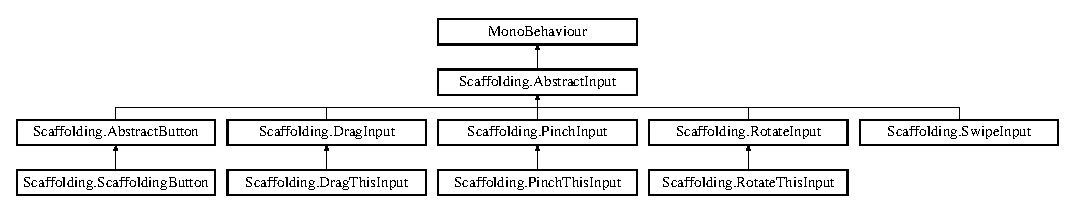
\includegraphics[height=2.395722cm]{class_scaffolding_1_1_abstract_input}
\end{center}
\end{figure}
\subsection*{Public Member Functions}
\begin{DoxyCompactItemize}
\item 
virtual void \hyperlink{class_scaffolding_1_1_abstract_input_a598859c6342920d2b0c985310e6e9476}{Setup} (\hyperlink{class_scaffolding_1_1_abstract_view}{Abstract\-View} view)
\begin{DoxyCompactList}\small\item\em Run by the view during it's setup phase. \end{DoxyCompactList}\item 
virtual void \hyperlink{class_scaffolding_1_1_abstract_input_a15d8f76fe4f335c622be311cfbec8b27}{On\-Destroy} ()
\begin{DoxyCompactList}\small\item\em When the input is destroyed, clean up after itself. \end{DoxyCompactList}\item 
virtual void \hyperlink{class_scaffolding_1_1_abstract_input_ab179ae99e76c6c934a0dcba4fc195e68}{Cleanup} ()
\begin{DoxyCompactList}\small\item\em The inputs clean up phase. \end{DoxyCompactList}\item 
virtual void \hyperlink{class_scaffolding_1_1_abstract_input_af1ca6d47fda48013c3521f106944d9af}{Kill} ()
\begin{DoxyCompactList}\small\item\em Removing any event references the input has \end{DoxyCompactList}\item 
virtual void \hyperlink{class_scaffolding_1_1_abstract_input_a5b19183daa9bbef63dd4637d7197c077}{Toggle\-Enabled\-Input} (bool enabled)
\begin{DoxyCompactList}\small\item\em Toggles the enabled state of the collider associated with the input. \end{DoxyCompactList}\item 
virtual void \hyperlink{class_scaffolding_1_1_abstract_input_a11e83c3462719749f8281a21024e902f}{Handle\-Event\-Pressed} (\hyperlink{class_scaffolding_1_1_input_tracker}{Input\-Tracker} tracker)
\begin{DoxyCompactList}\small\item\em Event\-Pressed, dispatched by Scaffoldings \hyperlink{class_scaffolding_1_1_input_manager}{Input\-Manager} Passes through a \hyperlink{class_scaffolding_1_1_input_tracker}{Input\-Tracker} of the current touch. \end{DoxyCompactList}\item 
virtual void \hyperlink{class_scaffolding_1_1_abstract_input_a11854454457cd55a26f345011f4bd6bc}{Handle\-Event\-Released} (\hyperlink{class_scaffolding_1_1_input_tracker}{Input\-Tracker} tracker)
\begin{DoxyCompactList}\small\item\em Event\-Released, dispatched by Scaffoldings \hyperlink{class_scaffolding_1_1_input_manager}{Input\-Manager} Passes through a \hyperlink{class_scaffolding_1_1_input_tracker}{Input\-Tracker} of the current touch. \end{DoxyCompactList}\item 
virtual void \hyperlink{class_scaffolding_1_1_abstract_input_a5996b0cb611a384e527ce871b9607858}{Handle\-Event\-Dragged} (\hyperlink{class_scaffolding_1_1_input_tracker}{Input\-Tracker} tracker)
\begin{DoxyCompactList}\small\item\em Event\-Dragged, dispatched by Scaffoldings \hyperlink{class_scaffolding_1_1_input_manager}{Input\-Manager} Passes through a \hyperlink{class_scaffolding_1_1_input_tracker}{Input\-Tracker} of the current touch. \end{DoxyCompactList}\item 
virtual void \hyperlink{class_scaffolding_1_1_abstract_input_a2f8eac0790f92d3ce70e196069cc6936}{Handle\-Event\-Dragged\-Delta} (Vector3 delta)
\begin{DoxyCompactList}\small\item\em Event\-Dragged, dispatched by Scaffoldings \hyperlink{class_scaffolding_1_1_input_manager}{Input\-Manager} Passes through an average delta position value of all known touches. \end{DoxyCompactList}\end{DoxyCompactItemize}


\subsection{Detailed Description}
Abstract input is responsible for all inputs responding to a touch or input from \hyperlink{class_scaffolding_1_1_input_manager}{Input\-Manager}. 



\subsection{Member Function Documentation}
\hypertarget{class_scaffolding_1_1_abstract_input_ab179ae99e76c6c934a0dcba4fc195e68}{\index{Scaffolding\-::\-Abstract\-Input@{Scaffolding\-::\-Abstract\-Input}!Cleanup@{Cleanup}}
\index{Cleanup@{Cleanup}!Scaffolding::AbstractInput@{Scaffolding\-::\-Abstract\-Input}}
\subsubsection[{Cleanup}]{\setlength{\rightskip}{0pt plus 5cm}virtual void Scaffolding.\-Abstract\-Input.\-Cleanup (
\begin{DoxyParamCaption}
{}
\end{DoxyParamCaption}
)\hspace{0.3cm}{\ttfamily [virtual]}}}\label{class_scaffolding_1_1_abstract_input_ab179ae99e76c6c934a0dcba4fc195e68}


The inputs clean up phase. 



Reimplemented in \hyperlink{class_scaffolding_1_1_scaffolding_button_a1f295926babd2653cd63ed2933108d45}{Scaffolding.\-Scaffolding\-Button}, \hyperlink{class_scaffolding_1_1_drag_input_aff15e6ed3bca67228c44918a544e241b}{Scaffolding.\-Drag\-Input}, \hyperlink{class_scaffolding_1_1_pinch_input_a5849a64ba0a49d679e4a57fc28fe3f7a}{Scaffolding.\-Pinch\-Input}, \hyperlink{class_scaffolding_1_1_rotate_input_a85778a91b86665998c1b84f24c571e88}{Scaffolding.\-Rotate\-Input}, and \hyperlink{class_scaffolding_1_1_swipe_input_a5d19c1744df90f14d150241605cb86bf}{Scaffolding.\-Swipe\-Input}.

\hypertarget{class_scaffolding_1_1_abstract_input_a5996b0cb611a384e527ce871b9607858}{\index{Scaffolding\-::\-Abstract\-Input@{Scaffolding\-::\-Abstract\-Input}!Handle\-Event\-Dragged@{Handle\-Event\-Dragged}}
\index{Handle\-Event\-Dragged@{Handle\-Event\-Dragged}!Scaffolding::AbstractInput@{Scaffolding\-::\-Abstract\-Input}}
\subsubsection[{Handle\-Event\-Dragged}]{\setlength{\rightskip}{0pt plus 5cm}virtual void Scaffolding.\-Abstract\-Input.\-Handle\-Event\-Dragged (
\begin{DoxyParamCaption}
\item[{{\bf Input\-Tracker}}]{tracker}
\end{DoxyParamCaption}
)\hspace{0.3cm}{\ttfamily [virtual]}}}\label{class_scaffolding_1_1_abstract_input_a5996b0cb611a384e527ce871b9607858}


Event\-Dragged, dispatched by Scaffoldings \hyperlink{class_scaffolding_1_1_input_manager}{Input\-Manager} Passes through a \hyperlink{class_scaffolding_1_1_input_tracker}{Input\-Tracker} of the current touch. 



Reimplemented in \hyperlink{class_scaffolding_1_1_swipe_input_a818aba4106a64b5dde4977bca4b358a7}{Scaffolding.\-Swipe\-Input}, \hyperlink{class_scaffolding_1_1_rotate_input_afffb85f2f27b314bde50d0e45d6117d5}{Scaffolding.\-Rotate\-Input}, and \hyperlink{class_scaffolding_1_1_pinch_input_a865f0201d2b7930241711abb68a7341d}{Scaffolding.\-Pinch\-Input}.

\hypertarget{class_scaffolding_1_1_abstract_input_a2f8eac0790f92d3ce70e196069cc6936}{\index{Scaffolding\-::\-Abstract\-Input@{Scaffolding\-::\-Abstract\-Input}!Handle\-Event\-Dragged\-Delta@{Handle\-Event\-Dragged\-Delta}}
\index{Handle\-Event\-Dragged\-Delta@{Handle\-Event\-Dragged\-Delta}!Scaffolding::AbstractInput@{Scaffolding\-::\-Abstract\-Input}}
\subsubsection[{Handle\-Event\-Dragged\-Delta}]{\setlength{\rightskip}{0pt plus 5cm}virtual void Scaffolding.\-Abstract\-Input.\-Handle\-Event\-Dragged\-Delta (
\begin{DoxyParamCaption}
\item[{Vector3}]{delta}
\end{DoxyParamCaption}
)\hspace{0.3cm}{\ttfamily [virtual]}}}\label{class_scaffolding_1_1_abstract_input_a2f8eac0790f92d3ce70e196069cc6936}


Event\-Dragged, dispatched by Scaffoldings \hyperlink{class_scaffolding_1_1_input_manager}{Input\-Manager} Passes through an average delta position value of all known touches. 



Reimplemented in \hyperlink{class_scaffolding_1_1_drag_input_a600650eb9b2e3ce954af6a5982db3360}{Scaffolding.\-Drag\-Input}.

\hypertarget{class_scaffolding_1_1_abstract_input_a11e83c3462719749f8281a21024e902f}{\index{Scaffolding\-::\-Abstract\-Input@{Scaffolding\-::\-Abstract\-Input}!Handle\-Event\-Pressed@{Handle\-Event\-Pressed}}
\index{Handle\-Event\-Pressed@{Handle\-Event\-Pressed}!Scaffolding::AbstractInput@{Scaffolding\-::\-Abstract\-Input}}
\subsubsection[{Handle\-Event\-Pressed}]{\setlength{\rightskip}{0pt plus 5cm}virtual void Scaffolding.\-Abstract\-Input.\-Handle\-Event\-Pressed (
\begin{DoxyParamCaption}
\item[{{\bf Input\-Tracker}}]{tracker}
\end{DoxyParamCaption}
)\hspace{0.3cm}{\ttfamily [virtual]}}}\label{class_scaffolding_1_1_abstract_input_a11e83c3462719749f8281a21024e902f}


Event\-Pressed, dispatched by Scaffoldings \hyperlink{class_scaffolding_1_1_input_manager}{Input\-Manager} Passes through a \hyperlink{class_scaffolding_1_1_input_tracker}{Input\-Tracker} of the current touch. 



Reimplemented in \hyperlink{class_scaffolding_1_1_drag_input_a49561ec761c72584711384d57cb74f41}{Scaffolding.\-Drag\-Input}, \hyperlink{class_scaffolding_1_1_scaffolding_button_a1cc1e5b6b74c5411e1ca46dd81eb5144}{Scaffolding.\-Scaffolding\-Button}, \hyperlink{class_scaffolding_1_1_rotate_input_a4c37089dcaae6d1cb1785b45d5cec8b3}{Scaffolding.\-Rotate\-Input}, \hyperlink{class_scaffolding_1_1_pinch_input_aea53be8e94bef95c8373dd05639eaa41}{Scaffolding.\-Pinch\-Input}, \hyperlink{class_scaffolding_1_1_pinch_this_input_a00f941bc53b1847a2be7a2e61a4a9a57}{Scaffolding.\-Pinch\-This\-Input}, \hyperlink{class_scaffolding_1_1_rotate_this_input_a721eb598cb78a1abb06d8c37f9de01ea}{Scaffolding.\-Rotate\-This\-Input}, and \hyperlink{class_scaffolding_1_1_drag_this_input_a09639007081a6fee7bb7141ec5fa32a5}{Scaffolding.\-Drag\-This\-Input}.

\hypertarget{class_scaffolding_1_1_abstract_input_a11854454457cd55a26f345011f4bd6bc}{\index{Scaffolding\-::\-Abstract\-Input@{Scaffolding\-::\-Abstract\-Input}!Handle\-Event\-Released@{Handle\-Event\-Released}}
\index{Handle\-Event\-Released@{Handle\-Event\-Released}!Scaffolding::AbstractInput@{Scaffolding\-::\-Abstract\-Input}}
\subsubsection[{Handle\-Event\-Released}]{\setlength{\rightskip}{0pt plus 5cm}virtual void Scaffolding.\-Abstract\-Input.\-Handle\-Event\-Released (
\begin{DoxyParamCaption}
\item[{{\bf Input\-Tracker}}]{tracker}
\end{DoxyParamCaption}
)\hspace{0.3cm}{\ttfamily [virtual]}}}\label{class_scaffolding_1_1_abstract_input_a11854454457cd55a26f345011f4bd6bc}


Event\-Released, dispatched by Scaffoldings \hyperlink{class_scaffolding_1_1_input_manager}{Input\-Manager} Passes through a \hyperlink{class_scaffolding_1_1_input_tracker}{Input\-Tracker} of the current touch. 



Reimplemented in \hyperlink{class_scaffolding_1_1_drag_input_ab50a7059961c803e39e3ce9ffb0945d7}{Scaffolding.\-Drag\-Input}, \hyperlink{class_scaffolding_1_1_scaffolding_button_ab6c3c337fc6c6c9dad69498ac5acd098}{Scaffolding.\-Scaffolding\-Button}, \hyperlink{class_scaffolding_1_1_rotate_input_a96588e29dafafeb2e1e1c5469b2bbda1}{Scaffolding.\-Rotate\-Input}, \hyperlink{class_scaffolding_1_1_pinch_input_ad7e6fa3689011526acda972b7f6f4aa8}{Scaffolding.\-Pinch\-Input}, \hyperlink{class_scaffolding_1_1_pinch_this_input_ad9ca7c0e4b14d3d59ff06b258b4b9f7d}{Scaffolding.\-Pinch\-This\-Input}, \hyperlink{class_scaffolding_1_1_drag_this_input_a9da2ff31ce625e9880e6f47cd8617c6a}{Scaffolding.\-Drag\-This\-Input}, and \hyperlink{class_scaffolding_1_1_rotate_this_input_aa90af18d3d575cb5a5176e3c952e68cd}{Scaffolding.\-Rotate\-This\-Input}.

\hypertarget{class_scaffolding_1_1_abstract_input_af1ca6d47fda48013c3521f106944d9af}{\index{Scaffolding\-::\-Abstract\-Input@{Scaffolding\-::\-Abstract\-Input}!Kill@{Kill}}
\index{Kill@{Kill}!Scaffolding::AbstractInput@{Scaffolding\-::\-Abstract\-Input}}
\subsubsection[{Kill}]{\setlength{\rightskip}{0pt plus 5cm}virtual void Scaffolding.\-Abstract\-Input.\-Kill (
\begin{DoxyParamCaption}
{}
\end{DoxyParamCaption}
)\hspace{0.3cm}{\ttfamily [virtual]}}}\label{class_scaffolding_1_1_abstract_input_af1ca6d47fda48013c3521f106944d9af}


Removing any event references the input has 

\hypertarget{class_scaffolding_1_1_abstract_input_a15d8f76fe4f335c622be311cfbec8b27}{\index{Scaffolding\-::\-Abstract\-Input@{Scaffolding\-::\-Abstract\-Input}!On\-Destroy@{On\-Destroy}}
\index{On\-Destroy@{On\-Destroy}!Scaffolding::AbstractInput@{Scaffolding\-::\-Abstract\-Input}}
\subsubsection[{On\-Destroy}]{\setlength{\rightskip}{0pt plus 5cm}virtual void Scaffolding.\-Abstract\-Input.\-On\-Destroy (
\begin{DoxyParamCaption}
{}
\end{DoxyParamCaption}
)\hspace{0.3cm}{\ttfamily [virtual]}}}\label{class_scaffolding_1_1_abstract_input_a15d8f76fe4f335c622be311cfbec8b27}


When the input is destroyed, clean up after itself. 

\hypertarget{class_scaffolding_1_1_abstract_input_a598859c6342920d2b0c985310e6e9476}{\index{Scaffolding\-::\-Abstract\-Input@{Scaffolding\-::\-Abstract\-Input}!Setup@{Setup}}
\index{Setup@{Setup}!Scaffolding::AbstractInput@{Scaffolding\-::\-Abstract\-Input}}
\subsubsection[{Setup}]{\setlength{\rightskip}{0pt plus 5cm}virtual void Scaffolding.\-Abstract\-Input.\-Setup (
\begin{DoxyParamCaption}
\item[{{\bf Abstract\-View}}]{view}
\end{DoxyParamCaption}
)\hspace{0.3cm}{\ttfamily [virtual]}}}\label{class_scaffolding_1_1_abstract_input_a598859c6342920d2b0c985310e6e9476}


Run by the view during it's setup phase. 



Reimplemented in \hyperlink{class_scaffolding_1_1_scaffolding_button_a9473252a76f28a9d9605c7be23377f94}{Scaffolding.\-Scaffolding\-Button}, \hyperlink{class_scaffolding_1_1_pinch_this_input_a60b5bc5461de1286d8bd142742451dab}{Scaffolding.\-Pinch\-This\-Input}, \hyperlink{class_scaffolding_1_1_drag_this_input_afb612ddc8d089c8708494b57063b235d}{Scaffolding.\-Drag\-This\-Input}, \hyperlink{class_scaffolding_1_1_rotate_this_input_a9e0fc73644310f1efd1f49e692638c89}{Scaffolding.\-Rotate\-This\-Input}, \hyperlink{class_scaffolding_1_1_pinch_input_aa6687d25d10c2f4e7106641e0647af35}{Scaffolding.\-Pinch\-Input}, and \hyperlink{class_scaffolding_1_1_rotate_input_a89be6ed5c624ff8f637fdc38227c4637}{Scaffolding.\-Rotate\-Input}.

\hypertarget{class_scaffolding_1_1_abstract_input_a5b19183daa9bbef63dd4637d7197c077}{\index{Scaffolding\-::\-Abstract\-Input@{Scaffolding\-::\-Abstract\-Input}!Toggle\-Enabled\-Input@{Toggle\-Enabled\-Input}}
\index{Toggle\-Enabled\-Input@{Toggle\-Enabled\-Input}!Scaffolding::AbstractInput@{Scaffolding\-::\-Abstract\-Input}}
\subsubsection[{Toggle\-Enabled\-Input}]{\setlength{\rightskip}{0pt plus 5cm}virtual void Scaffolding.\-Abstract\-Input.\-Toggle\-Enabled\-Input (
\begin{DoxyParamCaption}
\item[{bool}]{enabled}
\end{DoxyParamCaption}
)\hspace{0.3cm}{\ttfamily [virtual]}}}\label{class_scaffolding_1_1_abstract_input_a5b19183daa9bbef63dd4637d7197c077}


Toggles the enabled state of the collider associated with the input. 


\begin{DoxyParams}{Parameters}
{\em enabled} & If set to {\ttfamily true} enabled.\\
\hline
\end{DoxyParams}


Reimplemented in \hyperlink{class_scaffolding_1_1_scaffolding_button_aa84a30d26afd5a3f54b5614d6e09e535}{Scaffolding.\-Scaffolding\-Button}.



The documentation for this class was generated from the following file\-:\begin{DoxyCompactItemize}
\item 
Input/Abstract\-Input.\-cs\end{DoxyCompactItemize}

\hypertarget{class_scaffolding_1_1_abstract_model}{\section{Scaffolding.\+Abstract\+Model Class Reference}
\label{class_scaffolding_1_1_abstract_model}\index{Scaffolding.\+Abstract\+Model@{Scaffolding.\+Abstract\+Model}}
}


The default base of all automatically created models. Allows for easy registration between itself and its paired view, can also register other views.  


Inheritance diagram for Scaffolding.\+Abstract\+Model\+:\begin{figure}[H]
\begin{center}
\leavevmode
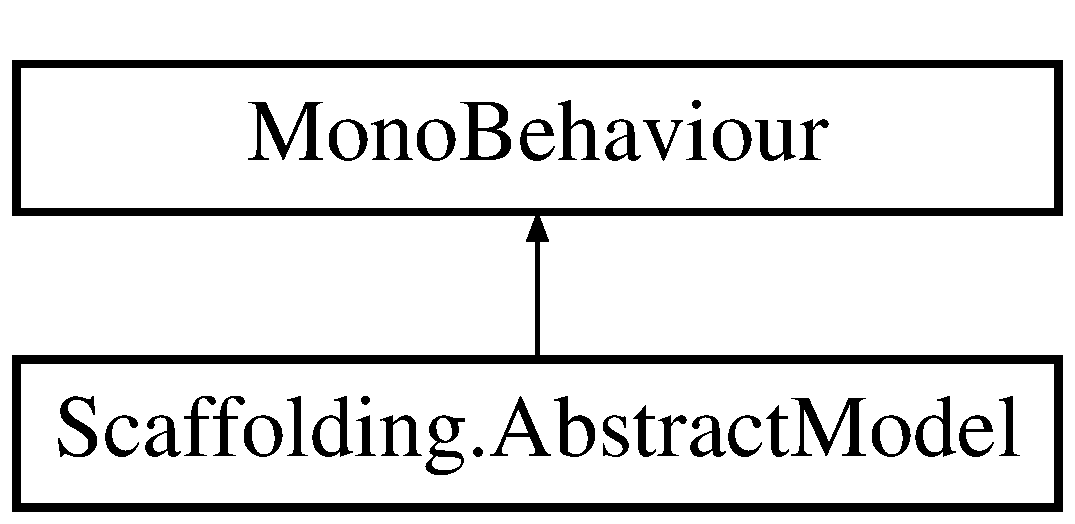
\includegraphics[height=2.000000cm]{class_scaffolding_1_1_abstract_model}
\end{center}
\end{figure}
\subsection*{Public Member Functions}
\begin{DoxyCompactItemize}
\item 
virtual void \hyperlink{class_scaffolding_1_1_abstract_model_a505c8e3a54070efd3c4a7d9016367fed}{Register\+View} (\hyperlink{class_scaffolding_1_1_abstract_view}{Abstract\+View} view)
\begin{DoxyCompactList}\small\item\em When the view associated with this model is opened, it gets registered with the model here. This also registers the default View\+Event delegate, for quick communication between registered views and the model. \end{DoxyCompactList}\item 
virtual void \hyperlink{class_scaffolding_1_1_abstract_model_af196af33f85f9dee1d6c37640e8631a6}{Handle\+View\+Closed\+Event} (\hyperlink{class_scaffolding_1_1_abstract_view}{Abstract\+View} sender, \hyperlink{class_scaffolding_1_1_s_object}{S\+Object} obj)
\begin{DoxyCompactList}\small\item\em Handles the view closed event. Automatically called when any view registered to this model is closed. This deregisters the view from the model. \end{DoxyCompactList}\item 
virtual void \hyperlink{class_scaffolding_1_1_abstract_model_a2a2f77959557dfd2983d4aca57fee9c4}{Handle\+View\+Event} (\hyperlink{class_scaffolding_1_1_abstract_view}{Abstract\+View} sender, \hyperlink{class_scaffolding_1_1_s_object}{S\+Object} obj)
\begin{DoxyCompactList}\small\item\em Handles the view event. Called by any view registered to the model. \end{DoxyCompactList}\item 
virtual void \hyperlink{class_scaffolding_1_1_abstract_model_a5ff673abdc32f2241d610050bfb57939}{View\+Closed} (\hyperlink{class_scaffolding_1_1_abstract_view}{Abstract\+View} view)
\begin{DoxyCompactList}\small\item\em Gets called when the view associated with this model is closed. \end{DoxyCompactList}\end{DoxyCompactItemize}


\subsection{Detailed Description}
The default base of all automatically created models. Allows for easy registration between itself and its paired view, can also register other views. 



\subsection{Member Function Documentation}
\hypertarget{class_scaffolding_1_1_abstract_model_af196af33f85f9dee1d6c37640e8631a6}{\index{Scaffolding\+::\+Abstract\+Model@{Scaffolding\+::\+Abstract\+Model}!Handle\+View\+Closed\+Event@{Handle\+View\+Closed\+Event}}
\index{Handle\+View\+Closed\+Event@{Handle\+View\+Closed\+Event}!Scaffolding\+::\+Abstract\+Model@{Scaffolding\+::\+Abstract\+Model}}
\subsubsection[{Handle\+View\+Closed\+Event}]{\setlength{\rightskip}{0pt plus 5cm}virtual void Scaffolding.\+Abstract\+Model.\+Handle\+View\+Closed\+Event (
\begin{DoxyParamCaption}
\item[{{\bf Abstract\+View}}]{sender, }
\item[{{\bf S\+Object}}]{obj}
\end{DoxyParamCaption}
)\hspace{0.3cm}{\ttfamily [virtual]}}}\label{class_scaffolding_1_1_abstract_model_af196af33f85f9dee1d6c37640e8631a6}


Handles the view closed event. Automatically called when any view registered to this model is closed. This deregisters the view from the model. 


\begin{DoxyParams}{Parameters}
{\em sender} & Sender.\\
\hline
{\em obj} & Object.\\
\hline
\end{DoxyParams}
\hypertarget{class_scaffolding_1_1_abstract_model_a2a2f77959557dfd2983d4aca57fee9c4}{\index{Scaffolding\+::\+Abstract\+Model@{Scaffolding\+::\+Abstract\+Model}!Handle\+View\+Event@{Handle\+View\+Event}}
\index{Handle\+View\+Event@{Handle\+View\+Event}!Scaffolding\+::\+Abstract\+Model@{Scaffolding\+::\+Abstract\+Model}}
\subsubsection[{Handle\+View\+Event}]{\setlength{\rightskip}{0pt plus 5cm}virtual void Scaffolding.\+Abstract\+Model.\+Handle\+View\+Event (
\begin{DoxyParamCaption}
\item[{{\bf Abstract\+View}}]{sender, }
\item[{{\bf S\+Object}}]{obj}
\end{DoxyParamCaption}
)\hspace{0.3cm}{\ttfamily [virtual]}}}\label{class_scaffolding_1_1_abstract_model_a2a2f77959557dfd2983d4aca57fee9c4}


Handles the view event. Called by any view registered to the model. 


\begin{DoxyParams}{Parameters}
{\em sender} & Sender.\\
\hline
{\em obj} & Object.\\
\hline
\end{DoxyParams}
\hypertarget{class_scaffolding_1_1_abstract_model_a505c8e3a54070efd3c4a7d9016367fed}{\index{Scaffolding\+::\+Abstract\+Model@{Scaffolding\+::\+Abstract\+Model}!Register\+View@{Register\+View}}
\index{Register\+View@{Register\+View}!Scaffolding\+::\+Abstract\+Model@{Scaffolding\+::\+Abstract\+Model}}
\subsubsection[{Register\+View}]{\setlength{\rightskip}{0pt plus 5cm}virtual void Scaffolding.\+Abstract\+Model.\+Register\+View (
\begin{DoxyParamCaption}
\item[{{\bf Abstract\+View}}]{view}
\end{DoxyParamCaption}
)\hspace{0.3cm}{\ttfamily [virtual]}}}\label{class_scaffolding_1_1_abstract_model_a505c8e3a54070efd3c4a7d9016367fed}


When the view associated with this model is opened, it gets registered with the model here. This also registers the default View\+Event delegate, for quick communication between registered views and the model. 


\begin{DoxyParams}{Parameters}
{\em view} & View.\\
\hline
\end{DoxyParams}
\hypertarget{class_scaffolding_1_1_abstract_model_a5ff673abdc32f2241d610050bfb57939}{\index{Scaffolding\+::\+Abstract\+Model@{Scaffolding\+::\+Abstract\+Model}!View\+Closed@{View\+Closed}}
\index{View\+Closed@{View\+Closed}!Scaffolding\+::\+Abstract\+Model@{Scaffolding\+::\+Abstract\+Model}}
\subsubsection[{View\+Closed}]{\setlength{\rightskip}{0pt plus 5cm}virtual void Scaffolding.\+Abstract\+Model.\+View\+Closed (
\begin{DoxyParamCaption}
\item[{{\bf Abstract\+View}}]{view}
\end{DoxyParamCaption}
)\hspace{0.3cm}{\ttfamily [virtual]}}}\label{class_scaffolding_1_1_abstract_model_a5ff673abdc32f2241d610050bfb57939}


Gets called when the view associated with this model is closed. 



The documentation for this class was generated from the following file\+:\begin{DoxyCompactItemize}
\item 
Views/Abstract\+Model.\+cs\end{DoxyCompactItemize}

\hypertarget{class_scaffolding_1_1_abstract_view}{\section{Scaffolding.\-Abstract\-View Class Reference}
\label{class_scaffolding_1_1_abstract_view}\index{Scaffolding.\-Abstract\-View@{Scaffolding.\-Abstract\-View}}
}


Abstract view. The base class for any view you wish to create, whether it is a Screen or Overlay.  


Inheritance diagram for Scaffolding.\-Abstract\-View\-:\begin{figure}[H]
\begin{center}
\leavevmode
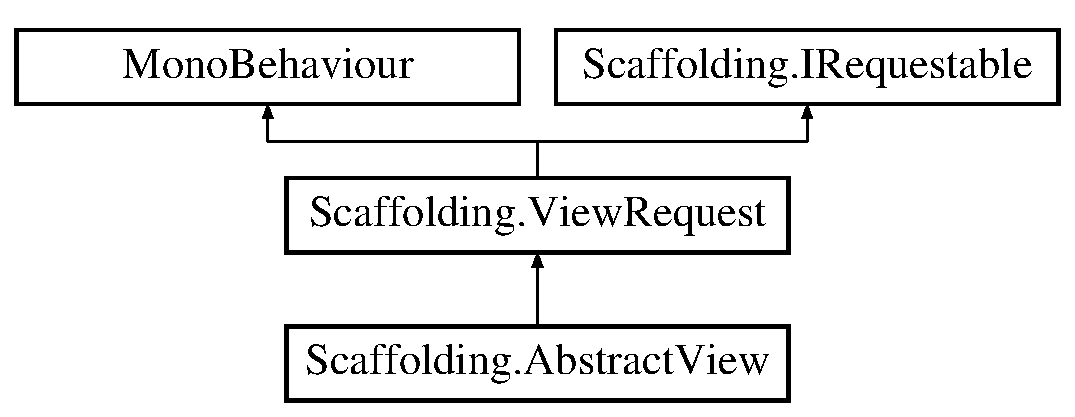
\includegraphics[height=2.000000cm]{class_scaffolding_1_1_abstract_view}
\end{center}
\end{figure}
\subsection*{Public Types}
\begin{DoxyCompactItemize}
\item 
enum {\bfseries Showing\-Types} \{ {\bfseries Wait\-For\-Previous\-Hide\-Transition}, 
{\bfseries Show\-Immediately}
 \}
\end{DoxyCompactItemize}
\subsection*{Public Member Functions}
\begin{DoxyCompactItemize}
\item 
\hyperlink{class_scaffolding_1_1_scaffolding_button}{Scaffolding\-Button} \hyperlink{class_scaffolding_1_1_abstract_view_a0d1b13f8a8b94985aecef73344b33270}{Get\-Button\-For\-Name} (string name)
\begin{DoxyCompactList}\small\item\em Return a button that is a child of the view by name. \end{DoxyCompactList}\item 
\hyperlink{class_scaffolding_1_1_s_object}{S\-Object} \hyperlink{class_scaffolding_1_1_abstract_view_a3acb31a04d6fa8d91358cb289cf12f28}{Get\-Data\-For\-Transition} (Type type)
\begin{DoxyCompactList}\small\item\em Get the data that has been packaged for delivery to a view. \end{DoxyCompactList}\item 
virtual void \hyperlink{class_scaffolding_1_1_abstract_view_adf0ec646b670c17b7635f21a74432332}{Setup} (\hyperlink{class_scaffolding_1_1_view_manager}{View\-Manager} manager)
\begin{DoxyCompactList}\small\item\em Runs when the view is created. Use this instead of Awake or Start. \end{DoxyCompactList}\item 
virtual void \hyperlink{class_scaffolding_1_1_abstract_view_a7c4ad4fbf3039a5acc67a16e6672510e}{On\-Show\-Start} (\hyperlink{class_scaffolding_1_1_s_object}{S\-Object} data)
\begin{DoxyCompactList}\small\item\em Runs when the view is opened, and before any animation events have happened. Any \hyperlink{class_scaffolding_1_1_abstract_input}{Abstract\-Input} derrived objects in the view are disabled at this point, to stop any clicks during the transitions. \end{DoxyCompactList}\item 
virtual void \hyperlink{class_scaffolding_1_1_abstract_view_ad3d0ee8b69a70afa3355c9aad0ab34b6}{On\-Show\-Complete} ()
\begin{DoxyCompactList}\small\item\em Runs after the \char`\"{}show\char`\"{} step has been completed, usually after any animations. Any \hyperlink{class_scaffolding_1_1_abstract_input}{Abstract\-Input} derrived objects in the view are enabled at this step. \end{DoxyCompactList}\item 
virtual void \hyperlink{class_scaffolding_1_1_abstract_view_ae8e198103d966b4a12bc8fdb27296765}{On\-Hide\-Start} ()
\begin{DoxyCompactList}\small\item\em Runs when the view is requested to close, before any animations. Any \hyperlink{class_scaffolding_1_1_abstract_input}{Abstract\-Input} derrived objects in the view are disabled at this point, to stop any clicks during the transitions. \end{DoxyCompactList}\item 
virtual void \hyperlink{class_scaffolding_1_1_abstract_view_aa5b29ad6a0a57677261e0bdc3b2e9825}{On\-Hide\-Complete} ()
\begin{DoxyCompactList}\small\item\em Runs when the view is completely closed. After this call, the view will be deleted. Any \hyperlink{class_scaffolding_1_1_abstract_input}{Abstract\-Input} derrived objects in the view are enabled at this step. \end{DoxyCompactList}\item 
virtual void \hyperlink{class_scaffolding_1_1_abstract_view_adfcc4c97dbec84c92718de4456717fc2}{Request\-Overlay} (Type type)
\begin{DoxyCompactList}\small\item\em Request an overlay with type to open. \end{DoxyCompactList}\item 
virtual void \hyperlink{class_scaffolding_1_1_abstract_view_a3b4879cd1667059f38599a7008d4fe61}{Request\-Overlay\-Close} (Type type)
\begin{DoxyCompactList}\small\item\em Request an overlay to close of type. \end{DoxyCompactList}\item 
virtual void \hyperlink{class_scaffolding_1_1_abstract_view_a5ad76f8f3445b4be40fe89a6e28d1d3b}{Request\-Overlay\-Force\-Close} (Type type)
\begin{DoxyCompactList}\small\item\em Force an overlay to close, this skips the On\-Hide\-Start method and goes straight to Hide\-Complete. \end{DoxyCompactList}\item 
virtual void \hyperlink{class_scaffolding_1_1_abstract_view_ac9e33d232d17e2815946bd7dfbdc718f}{Request\-View} (Type type)
\begin{DoxyCompactList}\small\item\em Request a view with type. \end{DoxyCompactList}\item 
virtual void \hyperlink{class_scaffolding_1_1_abstract_view_a4fce5dc780e682a9c32068dee4a4d58e}{Request\-View\-With\-Loading\-Overlay} (Type type, Type loading\-Type)
\begin{DoxyCompactList}\small\item\em Request a view, with an overlay. Used when the requested view is a heavy load and you want to mask that stall with a loading screen. \end{DoxyCompactList}\item 
void \hyperlink{class_scaffolding_1_1_abstract_view_a5676805d5374e27b0903a49fece06021}{Send\-Data\-To\-View} (Type target\-View, \hyperlink{class_scaffolding_1_1_s_object}{S\-Object} data)
\begin{DoxyCompactList}\small\item\em Package up data to send to a target view. Useful to send data between views, can be packaged anytime before the change view request happens. \end{DoxyCompactList}\item 
void \hyperlink{class_scaffolding_1_1_abstract_view_ac150377c429c981707547230cf2ccb73}{Remove\-Data\-For\-View} (Type target\-View)
\begin{DoxyCompactList}\small\item\em Delete any data you want to send to a view. \end{DoxyCompactList}\item 
void \hyperlink{class_scaffolding_1_1_abstract_view_a1bb34cd891cb97082030215fdb8b8794}{Disable\-All\-Inputs} ()
\begin{DoxyCompactList}\small\item\em Disable any inputs found in the view. \end{DoxyCompactList}\item 
void \hyperlink{class_scaffolding_1_1_abstract_view_ae550b6838501b3c2e3751535059c478e}{Enable\-All\-Inputs} ()
\begin{DoxyCompactList}\small\item\em Enable any inputs found in the view. \end{DoxyCompactList}\item 
void \hyperlink{class_scaffolding_1_1_abstract_view_a5e6cdf214eaa49da7ef180c6874353b0}{Toggle\-Enabled\-Inputs} (bool enabled)
\begin{DoxyCompactList}\small\item\em Toggles the enabled state of all inputs in the view. \end{DoxyCompactList}\end{DoxyCompactItemize}
\subsection*{Public Attributes}
\begin{DoxyCompactItemize}
\item 
\hypertarget{class_scaffolding_1_1_abstract_view_a7a3bdf62bce105b7857671d30adb179b}{Showing\-Types {\bfseries showing\-Type}}\label{class_scaffolding_1_1_abstract_view_a7a3bdf62bce105b7857671d30adb179b}

\item 
\hypertarget{class_scaffolding_1_1_abstract_view_addde808d8caa8a49014303bf1dcc1f8e}{Animation\-Clip {\bfseries in\-Transition}}\label{class_scaffolding_1_1_abstract_view_addde808d8caa8a49014303bf1dcc1f8e}

\item 
\hypertarget{class_scaffolding_1_1_abstract_view_aa62967668127d7526d2bca78e1e1501b}{Animation\-Clip {\bfseries out\-Transition}}\label{class_scaffolding_1_1_abstract_view_aa62967668127d7526d2bca78e1e1501b}

\item 
\hypertarget{class_scaffolding_1_1_abstract_view_ae03980c52528bdb18b92932bb1f17e7b}{bool {\bfseries disable\-Inputs\-If\-Overlay}}\label{class_scaffolding_1_1_abstract_view_ae03980c52528bdb18b92932bb1f17e7b}

\end{DoxyCompactItemize}
\subsection*{Properties}
\begin{DoxyCompactItemize}
\item 
bool \hyperlink{class_scaffolding_1_1_abstract_view_a162a5103cff0b5aa7938715e1a84ad61}{Is\-Hiding}\hspace{0.3cm}{\ttfamily  \mbox{[}get\mbox{]}}
\begin{DoxyCompactList}\small\item\em Gets a value indicating whether or not this view is in the hide state. \end{DoxyCompactList}\item 
bool \hyperlink{class_scaffolding_1_1_abstract_view_ac933ea22f4d4b9e511f872d53d37a544}{Is\-Showing}\hspace{0.3cm}{\ttfamily  \mbox{[}get\mbox{]}}
\begin{DoxyCompactList}\small\item\em Gets a value indicating whether or not this view is in the showing state. \end{DoxyCompactList}\end{DoxyCompactItemize}


\subsection{Detailed Description}
Abstract view. The base class for any view you wish to create, whether it is a Screen or Overlay. 



\subsection{Member Function Documentation}
\hypertarget{class_scaffolding_1_1_abstract_view_a1bb34cd891cb97082030215fdb8b8794}{\index{Scaffolding\-::\-Abstract\-View@{Scaffolding\-::\-Abstract\-View}!Disable\-All\-Inputs@{Disable\-All\-Inputs}}
\index{Disable\-All\-Inputs@{Disable\-All\-Inputs}!Scaffolding::AbstractView@{Scaffolding\-::\-Abstract\-View}}
\subsubsection[{Disable\-All\-Inputs}]{\setlength{\rightskip}{0pt plus 5cm}void Scaffolding.\-Abstract\-View.\-Disable\-All\-Inputs (
\begin{DoxyParamCaption}
{}
\end{DoxyParamCaption}
)}}\label{class_scaffolding_1_1_abstract_view_a1bb34cd891cb97082030215fdb8b8794}


Disable any inputs found in the view. 

\hypertarget{class_scaffolding_1_1_abstract_view_ae550b6838501b3c2e3751535059c478e}{\index{Scaffolding\-::\-Abstract\-View@{Scaffolding\-::\-Abstract\-View}!Enable\-All\-Inputs@{Enable\-All\-Inputs}}
\index{Enable\-All\-Inputs@{Enable\-All\-Inputs}!Scaffolding::AbstractView@{Scaffolding\-::\-Abstract\-View}}
\subsubsection[{Enable\-All\-Inputs}]{\setlength{\rightskip}{0pt plus 5cm}void Scaffolding.\-Abstract\-View.\-Enable\-All\-Inputs (
\begin{DoxyParamCaption}
{}
\end{DoxyParamCaption}
)}}\label{class_scaffolding_1_1_abstract_view_ae550b6838501b3c2e3751535059c478e}


Enable any inputs found in the view. 

\hypertarget{class_scaffolding_1_1_abstract_view_a0d1b13f8a8b94985aecef73344b33270}{\index{Scaffolding\-::\-Abstract\-View@{Scaffolding\-::\-Abstract\-View}!Get\-Button\-For\-Name@{Get\-Button\-For\-Name}}
\index{Get\-Button\-For\-Name@{Get\-Button\-For\-Name}!Scaffolding::AbstractView@{Scaffolding\-::\-Abstract\-View}}
\subsubsection[{Get\-Button\-For\-Name}]{\setlength{\rightskip}{0pt plus 5cm}{\bf Scaffolding\-Button} Scaffolding.\-Abstract\-View.\-Get\-Button\-For\-Name (
\begin{DoxyParamCaption}
\item[{string}]{name}
\end{DoxyParamCaption}
)}}\label{class_scaffolding_1_1_abstract_view_a0d1b13f8a8b94985aecef73344b33270}


Return a button that is a child of the view by name. 

\hypertarget{class_scaffolding_1_1_abstract_view_a3acb31a04d6fa8d91358cb289cf12f28}{\index{Scaffolding\-::\-Abstract\-View@{Scaffolding\-::\-Abstract\-View}!Get\-Data\-For\-Transition@{Get\-Data\-For\-Transition}}
\index{Get\-Data\-For\-Transition@{Get\-Data\-For\-Transition}!Scaffolding::AbstractView@{Scaffolding\-::\-Abstract\-View}}
\subsubsection[{Get\-Data\-For\-Transition}]{\setlength{\rightskip}{0pt plus 5cm}{\bf S\-Object} Scaffolding.\-Abstract\-View.\-Get\-Data\-For\-Transition (
\begin{DoxyParamCaption}
\item[{Type}]{type}
\end{DoxyParamCaption}
)}}\label{class_scaffolding_1_1_abstract_view_a3acb31a04d6fa8d91358cb289cf12f28}


Get the data that has been packaged for delivery to a view. 

\hypertarget{class_scaffolding_1_1_abstract_view_aa5b29ad6a0a57677261e0bdc3b2e9825}{\index{Scaffolding\-::\-Abstract\-View@{Scaffolding\-::\-Abstract\-View}!On\-Hide\-Complete@{On\-Hide\-Complete}}
\index{On\-Hide\-Complete@{On\-Hide\-Complete}!Scaffolding::AbstractView@{Scaffolding\-::\-Abstract\-View}}
\subsubsection[{On\-Hide\-Complete}]{\setlength{\rightskip}{0pt plus 5cm}virtual void Scaffolding.\-Abstract\-View.\-On\-Hide\-Complete (
\begin{DoxyParamCaption}
{}
\end{DoxyParamCaption}
)\hspace{0.3cm}{\ttfamily [virtual]}}}\label{class_scaffolding_1_1_abstract_view_aa5b29ad6a0a57677261e0bdc3b2e9825}


Runs when the view is completely closed. After this call, the view will be deleted. Any \hyperlink{class_scaffolding_1_1_abstract_input}{Abstract\-Input} derrived objects in the view are enabled at this step. 

\hypertarget{class_scaffolding_1_1_abstract_view_ae8e198103d966b4a12bc8fdb27296765}{\index{Scaffolding\-::\-Abstract\-View@{Scaffolding\-::\-Abstract\-View}!On\-Hide\-Start@{On\-Hide\-Start}}
\index{On\-Hide\-Start@{On\-Hide\-Start}!Scaffolding::AbstractView@{Scaffolding\-::\-Abstract\-View}}
\subsubsection[{On\-Hide\-Start}]{\setlength{\rightskip}{0pt plus 5cm}virtual void Scaffolding.\-Abstract\-View.\-On\-Hide\-Start (
\begin{DoxyParamCaption}
{}
\end{DoxyParamCaption}
)\hspace{0.3cm}{\ttfamily [virtual]}}}\label{class_scaffolding_1_1_abstract_view_ae8e198103d966b4a12bc8fdb27296765}


Runs when the view is requested to close, before any animations. Any \hyperlink{class_scaffolding_1_1_abstract_input}{Abstract\-Input} derrived objects in the view are disabled at this point, to stop any clicks during the transitions. 

\hypertarget{class_scaffolding_1_1_abstract_view_ad3d0ee8b69a70afa3355c9aad0ab34b6}{\index{Scaffolding\-::\-Abstract\-View@{Scaffolding\-::\-Abstract\-View}!On\-Show\-Complete@{On\-Show\-Complete}}
\index{On\-Show\-Complete@{On\-Show\-Complete}!Scaffolding::AbstractView@{Scaffolding\-::\-Abstract\-View}}
\subsubsection[{On\-Show\-Complete}]{\setlength{\rightskip}{0pt plus 5cm}virtual void Scaffolding.\-Abstract\-View.\-On\-Show\-Complete (
\begin{DoxyParamCaption}
{}
\end{DoxyParamCaption}
)\hspace{0.3cm}{\ttfamily [virtual]}}}\label{class_scaffolding_1_1_abstract_view_ad3d0ee8b69a70afa3355c9aad0ab34b6}


Runs after the \char`\"{}show\char`\"{} step has been completed, usually after any animations. Any \hyperlink{class_scaffolding_1_1_abstract_input}{Abstract\-Input} derrived objects in the view are enabled at this step. 

\hypertarget{class_scaffolding_1_1_abstract_view_a7c4ad4fbf3039a5acc67a16e6672510e}{\index{Scaffolding\-::\-Abstract\-View@{Scaffolding\-::\-Abstract\-View}!On\-Show\-Start@{On\-Show\-Start}}
\index{On\-Show\-Start@{On\-Show\-Start}!Scaffolding::AbstractView@{Scaffolding\-::\-Abstract\-View}}
\subsubsection[{On\-Show\-Start}]{\setlength{\rightskip}{0pt plus 5cm}virtual void Scaffolding.\-Abstract\-View.\-On\-Show\-Start (
\begin{DoxyParamCaption}
\item[{{\bf S\-Object}}]{data}
\end{DoxyParamCaption}
)\hspace{0.3cm}{\ttfamily [virtual]}}}\label{class_scaffolding_1_1_abstract_view_a7c4ad4fbf3039a5acc67a16e6672510e}


Runs when the view is opened, and before any animation events have happened. Any \hyperlink{class_scaffolding_1_1_abstract_input}{Abstract\-Input} derrived objects in the view are disabled at this point, to stop any clicks during the transitions. 

\hypertarget{class_scaffolding_1_1_abstract_view_ac150377c429c981707547230cf2ccb73}{\index{Scaffolding\-::\-Abstract\-View@{Scaffolding\-::\-Abstract\-View}!Remove\-Data\-For\-View@{Remove\-Data\-For\-View}}
\index{Remove\-Data\-For\-View@{Remove\-Data\-For\-View}!Scaffolding::AbstractView@{Scaffolding\-::\-Abstract\-View}}
\subsubsection[{Remove\-Data\-For\-View}]{\setlength{\rightskip}{0pt plus 5cm}void Scaffolding.\-Abstract\-View.\-Remove\-Data\-For\-View (
\begin{DoxyParamCaption}
\item[{Type}]{target\-View}
\end{DoxyParamCaption}
)}}\label{class_scaffolding_1_1_abstract_view_ac150377c429c981707547230cf2ccb73}


Delete any data you want to send to a view. 


\begin{DoxyParams}{Parameters}
{\em target\-View} & Target view.\\
\hline
\end{DoxyParams}
\hypertarget{class_scaffolding_1_1_abstract_view_adfcc4c97dbec84c92718de4456717fc2}{\index{Scaffolding\-::\-Abstract\-View@{Scaffolding\-::\-Abstract\-View}!Request\-Overlay@{Request\-Overlay}}
\index{Request\-Overlay@{Request\-Overlay}!Scaffolding::AbstractView@{Scaffolding\-::\-Abstract\-View}}
\subsubsection[{Request\-Overlay}]{\setlength{\rightskip}{0pt plus 5cm}virtual void Scaffolding.\-Abstract\-View.\-Request\-Overlay (
\begin{DoxyParamCaption}
\item[{Type}]{type}
\end{DoxyParamCaption}
)\hspace{0.3cm}{\ttfamily [virtual]}}}\label{class_scaffolding_1_1_abstract_view_adfcc4c97dbec84c92718de4456717fc2}


Request an overlay with type to open. 

Example\-: Request\-Overlay(typeof(\-My\-View)); \hypertarget{class_scaffolding_1_1_abstract_view_a3b4879cd1667059f38599a7008d4fe61}{\index{Scaffolding\-::\-Abstract\-View@{Scaffolding\-::\-Abstract\-View}!Request\-Overlay\-Close@{Request\-Overlay\-Close}}
\index{Request\-Overlay\-Close@{Request\-Overlay\-Close}!Scaffolding::AbstractView@{Scaffolding\-::\-Abstract\-View}}
\subsubsection[{Request\-Overlay\-Close}]{\setlength{\rightskip}{0pt plus 5cm}virtual void Scaffolding.\-Abstract\-View.\-Request\-Overlay\-Close (
\begin{DoxyParamCaption}
\item[{Type}]{type}
\end{DoxyParamCaption}
)\hspace{0.3cm}{\ttfamily [virtual]}}}\label{class_scaffolding_1_1_abstract_view_a3b4879cd1667059f38599a7008d4fe61}


Request an overlay to close of type. 

Example\-: Request\-Overlay\-Close(typeof(\-My\-View)); \hypertarget{class_scaffolding_1_1_abstract_view_a5ad76f8f3445b4be40fe89a6e28d1d3b}{\index{Scaffolding\-::\-Abstract\-View@{Scaffolding\-::\-Abstract\-View}!Request\-Overlay\-Force\-Close@{Request\-Overlay\-Force\-Close}}
\index{Request\-Overlay\-Force\-Close@{Request\-Overlay\-Force\-Close}!Scaffolding::AbstractView@{Scaffolding\-::\-Abstract\-View}}
\subsubsection[{Request\-Overlay\-Force\-Close}]{\setlength{\rightskip}{0pt plus 5cm}virtual void Scaffolding.\-Abstract\-View.\-Request\-Overlay\-Force\-Close (
\begin{DoxyParamCaption}
\item[{Type}]{type}
\end{DoxyParamCaption}
)\hspace{0.3cm}{\ttfamily [virtual]}}}\label{class_scaffolding_1_1_abstract_view_a5ad76f8f3445b4be40fe89a6e28d1d3b}


Force an overlay to close, this skips the On\-Hide\-Start method and goes straight to Hide\-Complete. 

Example\-: Request\-Overlay\-Force\-Close(typeof(\-My\-View)); \hypertarget{class_scaffolding_1_1_abstract_view_ac9e33d232d17e2815946bd7dfbdc718f}{\index{Scaffolding\-::\-Abstract\-View@{Scaffolding\-::\-Abstract\-View}!Request\-View@{Request\-View}}
\index{Request\-View@{Request\-View}!Scaffolding::AbstractView@{Scaffolding\-::\-Abstract\-View}}
\subsubsection[{Request\-View}]{\setlength{\rightskip}{0pt plus 5cm}virtual void Scaffolding.\-Abstract\-View.\-Request\-View (
\begin{DoxyParamCaption}
\item[{Type}]{type}
\end{DoxyParamCaption}
)\hspace{0.3cm}{\ttfamily [virtual]}}}\label{class_scaffolding_1_1_abstract_view_ac9e33d232d17e2815946bd7dfbdc718f}


Request a view with type. 

Example\-: Request\-View(typeof(\-My\-View)); \hypertarget{class_scaffolding_1_1_abstract_view_a4fce5dc780e682a9c32068dee4a4d58e}{\index{Scaffolding\-::\-Abstract\-View@{Scaffolding\-::\-Abstract\-View}!Request\-View\-With\-Loading\-Overlay@{Request\-View\-With\-Loading\-Overlay}}
\index{Request\-View\-With\-Loading\-Overlay@{Request\-View\-With\-Loading\-Overlay}!Scaffolding::AbstractView@{Scaffolding\-::\-Abstract\-View}}
\subsubsection[{Request\-View\-With\-Loading\-Overlay}]{\setlength{\rightskip}{0pt plus 5cm}virtual void Scaffolding.\-Abstract\-View.\-Request\-View\-With\-Loading\-Overlay (
\begin{DoxyParamCaption}
\item[{Type}]{type, }
\item[{Type}]{loading\-Type}
\end{DoxyParamCaption}
)\hspace{0.3cm}{\ttfamily [virtual]}}}\label{class_scaffolding_1_1_abstract_view_a4fce5dc780e682a9c32068dee4a4d58e}


Request a view, with an overlay. Used when the requested view is a heavy load and you want to mask that stall with a loading screen. 

Example\-: Request\-View\-With\-Loading\-Overlay(typeof(\-My\-Heavy\-View),typeof(\-My\-Loading\-Screen)); \hypertarget{class_scaffolding_1_1_abstract_view_a5676805d5374e27b0903a49fece06021}{\index{Scaffolding\-::\-Abstract\-View@{Scaffolding\-::\-Abstract\-View}!Send\-Data\-To\-View@{Send\-Data\-To\-View}}
\index{Send\-Data\-To\-View@{Send\-Data\-To\-View}!Scaffolding::AbstractView@{Scaffolding\-::\-Abstract\-View}}
\subsubsection[{Send\-Data\-To\-View}]{\setlength{\rightskip}{0pt plus 5cm}void Scaffolding.\-Abstract\-View.\-Send\-Data\-To\-View (
\begin{DoxyParamCaption}
\item[{Type}]{target\-View, }
\item[{{\bf S\-Object}}]{data}
\end{DoxyParamCaption}
)}}\label{class_scaffolding_1_1_abstract_view_a5676805d5374e27b0903a49fece06021}


Package up data to send to a target view. Useful to send data between views, can be packaged anytime before the change view request happens. 

Example\-: Value\-Object obj = new Value\-Object(); obj.\-Put\-Int(\char`\"{}\-Key\char`\"{}, 10); Send\-Data\-To\-View(type\-Of(\-My\-View),obj); \hypertarget{class_scaffolding_1_1_abstract_view_adf0ec646b670c17b7635f21a74432332}{\index{Scaffolding\-::\-Abstract\-View@{Scaffolding\-::\-Abstract\-View}!Setup@{Setup}}
\index{Setup@{Setup}!Scaffolding::AbstractView@{Scaffolding\-::\-Abstract\-View}}
\subsubsection[{Setup}]{\setlength{\rightskip}{0pt plus 5cm}virtual void Scaffolding.\-Abstract\-View.\-Setup (
\begin{DoxyParamCaption}
\item[{{\bf View\-Manager}}]{manager}
\end{DoxyParamCaption}
)\hspace{0.3cm}{\ttfamily [virtual]}}}\label{class_scaffolding_1_1_abstract_view_adf0ec646b670c17b7635f21a74432332}


Runs when the view is created. Use this instead of Awake or Start. 

\hypertarget{class_scaffolding_1_1_abstract_view_a5e6cdf214eaa49da7ef180c6874353b0}{\index{Scaffolding\-::\-Abstract\-View@{Scaffolding\-::\-Abstract\-View}!Toggle\-Enabled\-Inputs@{Toggle\-Enabled\-Inputs}}
\index{Toggle\-Enabled\-Inputs@{Toggle\-Enabled\-Inputs}!Scaffolding::AbstractView@{Scaffolding\-::\-Abstract\-View}}
\subsubsection[{Toggle\-Enabled\-Inputs}]{\setlength{\rightskip}{0pt plus 5cm}void Scaffolding.\-Abstract\-View.\-Toggle\-Enabled\-Inputs (
\begin{DoxyParamCaption}
\item[{bool}]{enabled}
\end{DoxyParamCaption}
)}}\label{class_scaffolding_1_1_abstract_view_a5e6cdf214eaa49da7ef180c6874353b0}


Toggles the enabled state of all inputs in the view. 


\begin{DoxyParams}{Parameters}
{\em enabled} & If set to {\ttfamily true} enabled.\\
\hline
\end{DoxyParams}


\subsection{Property Documentation}
\hypertarget{class_scaffolding_1_1_abstract_view_a162a5103cff0b5aa7938715e1a84ad61}{\index{Scaffolding\-::\-Abstract\-View@{Scaffolding\-::\-Abstract\-View}!Is\-Hiding@{Is\-Hiding}}
\index{Is\-Hiding@{Is\-Hiding}!Scaffolding::AbstractView@{Scaffolding\-::\-Abstract\-View}}
\subsubsection[{Is\-Hiding}]{\setlength{\rightskip}{0pt plus 5cm}bool Scaffolding.\-Abstract\-View.\-Is\-Hiding\hspace{0.3cm}{\ttfamily [get]}}}\label{class_scaffolding_1_1_abstract_view_a162a5103cff0b5aa7938715e1a84ad61}


Gets a value indicating whether or not this view is in the hide state. 

{\ttfamily true} if this instance is hiding; otherwise, {\ttfamily false}.\hypertarget{class_scaffolding_1_1_abstract_view_ac933ea22f4d4b9e511f872d53d37a544}{\index{Scaffolding\-::\-Abstract\-View@{Scaffolding\-::\-Abstract\-View}!Is\-Showing@{Is\-Showing}}
\index{Is\-Showing@{Is\-Showing}!Scaffolding::AbstractView@{Scaffolding\-::\-Abstract\-View}}
\subsubsection[{Is\-Showing}]{\setlength{\rightskip}{0pt plus 5cm}bool Scaffolding.\-Abstract\-View.\-Is\-Showing\hspace{0.3cm}{\ttfamily [get]}}}\label{class_scaffolding_1_1_abstract_view_ac933ea22f4d4b9e511f872d53d37a544}


Gets a value indicating whether or not this view is in the showing state. 

{\ttfamily true} if this instance is showing; otherwise, {\ttfamily false}.

The documentation for this class was generated from the following file\-:\begin{DoxyCompactItemize}
\item 
Location/Abstract\-View.\-cs\end{DoxyCompactItemize}

\hypertarget{class_scaffolding_1_1_drag_input}{\section{Scaffolding.\-Drag\-Input Class Reference}
\label{class_scaffolding_1_1_drag_input}\index{Scaffolding.\-Drag\-Input@{Scaffolding.\-Drag\-Input}}
}


Drag input is a quick dragging solution using \hyperlink{class_scaffolding_1_1_abstract_input}{Abstract\-Input}.  


Inheritance diagram for Scaffolding.\-Drag\-Input\-:\begin{figure}[H]
\begin{center}
\leavevmode
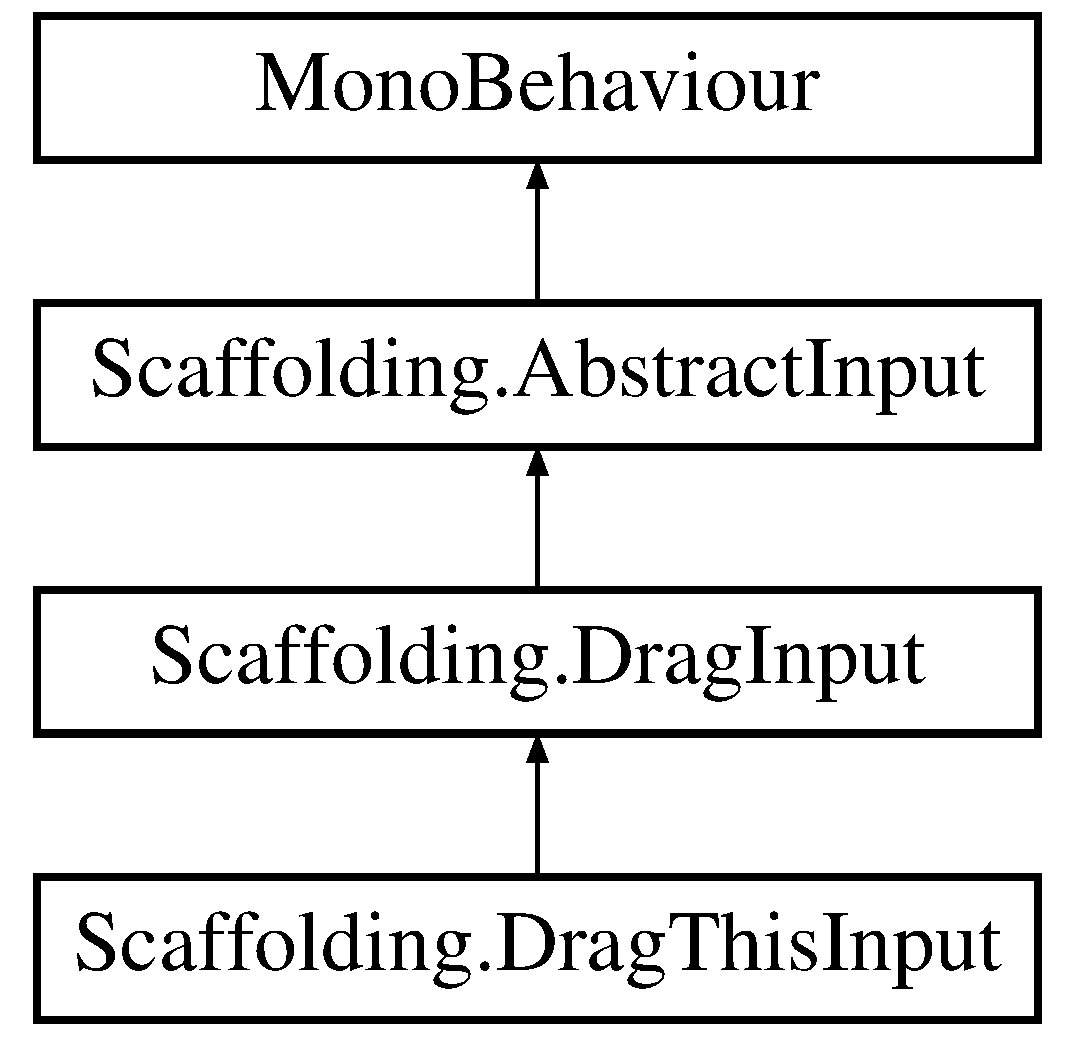
\includegraphics[height=4.000000cm]{class_scaffolding_1_1_drag_input}
\end{center}
\end{figure}
\subsection*{Public Member Functions}
\begin{DoxyCompactItemize}
\item 
override void \hyperlink{class_scaffolding_1_1_drag_input_aff15e6ed3bca67228c44918a544e241b}{Cleanup} ()
\begin{DoxyCompactList}\small\item\em The inputs clean up phase. \end{DoxyCompactList}\item 
void \hyperlink{class_scaffolding_1_1_drag_input_aa14faf0a305db966f957bb59ab5de1ff}{Register\-Drag\-Callback} (Action$<$ Vector3 $>$ callback)
\begin{DoxyCompactList}\small\item\em Registers the drag callback. \end{DoxyCompactList}\item 
void \hyperlink{class_scaffolding_1_1_drag_input_a5f46ef8ef277a59f91ce14eb725af851}{Register\-Direction\-Callback} (Action$<$ Direction $>$ callback)
\begin{DoxyCompactList}\small\item\em Registers the direction callback. \end{DoxyCompactList}\item 
override void \hyperlink{class_scaffolding_1_1_drag_input_a600650eb9b2e3ce954af6a5982db3360}{Handle\-Event\-Dragged\-Delta} (Vector3 delta)
\begin{DoxyCompactList}\small\item\em Event\-Dragged, dispatched by Scaffoldings \hyperlink{class_scaffolding_1_1_input_manager}{Input\-Manager} Passes through an average delta position value of all known touches. \end{DoxyCompactList}\item 
override void \hyperlink{class_scaffolding_1_1_drag_input_a49561ec761c72584711384d57cb74f41}{Handle\-Event\-Pressed} (\hyperlink{class_scaffolding_1_1_input_tracker}{Input\-Tracker} tracker)
\begin{DoxyCompactList}\small\item\em Event\-Pressed, dispatched by Scaffoldings \hyperlink{class_scaffolding_1_1_input_manager}{Input\-Manager} Passes through a \hyperlink{class_scaffolding_1_1_input_tracker}{Input\-Tracker} of the current touch. \end{DoxyCompactList}\item 
override void \hyperlink{class_scaffolding_1_1_drag_input_ab50a7059961c803e39e3ce9ffb0945d7}{Handle\-Event\-Released} (\hyperlink{class_scaffolding_1_1_input_tracker}{Input\-Tracker} tracker)
\begin{DoxyCompactList}\small\item\em Event\-Released, dispatched by Scaffoldings \hyperlink{class_scaffolding_1_1_input_manager}{Input\-Manager} Passes through a \hyperlink{class_scaffolding_1_1_input_tracker}{Input\-Tracker} of the current touch. \end{DoxyCompactList}\end{DoxyCompactItemize}
\subsection*{Public Attributes}
\begin{DoxyCompactItemize}
\item 
\hypertarget{class_scaffolding_1_1_drag_input_a4f032b5cb00663f311d36154fb8e64a3}{bool {\bfseries lock\-Horizontal}}\label{class_scaffolding_1_1_drag_input_a4f032b5cb00663f311d36154fb8e64a3}

\item 
\hypertarget{class_scaffolding_1_1_drag_input_ab1eb142a4d7572c0c1cc36b2a50d7eee}{bool {\bfseries lock\-Vertical}}\label{class_scaffolding_1_1_drag_input_ab1eb142a4d7572c0c1cc36b2a50d7eee}

\end{DoxyCompactItemize}
\subsection*{Properties}
\begin{DoxyCompactItemize}
\item 
bool \hyperlink{class_scaffolding_1_1_drag_input_ab8e2d83d121fbd2b3ad60ef23fe5332f}{Mouse\-Pressed}\hspace{0.3cm}{\ttfamily  \mbox{[}get\mbox{]}}
\begin{DoxyCompactList}\small\item\em Gets a value indicating whether this \hyperlink{class_scaffolding_1_1_drag_input}{Scaffolding.\-Drag\-Input} mouse pressed. \end{DoxyCompactList}\item 
bool \hyperlink{class_scaffolding_1_1_drag_input_ab13911d3778d99a0687b7bf724adb42d}{Lock\-Horizontal}\hspace{0.3cm}{\ttfamily  \mbox{[}get, set\mbox{]}}
\begin{DoxyCompactList}\small\item\em Gets or sets a value indicating whether this \hyperlink{class_scaffolding_1_1_drag_input}{Scaffolding.\-Drag\-Input} lock horizontal. \end{DoxyCompactList}\item 
bool \hyperlink{class_scaffolding_1_1_drag_input_a5efcdda6db82447e4e61490c85977180}{Lock\-Vertical}\hspace{0.3cm}{\ttfamily  \mbox{[}get, set\mbox{]}}
\begin{DoxyCompactList}\small\item\em Gets or sets a value indicating whether this \hyperlink{class_scaffolding_1_1_drag_input}{Scaffolding.\-Drag\-Input} lock vertical. \end{DoxyCompactList}\end{DoxyCompactItemize}


\subsection{Detailed Description}
Drag input is a quick dragging solution using \hyperlink{class_scaffolding_1_1_abstract_input}{Abstract\-Input}. 



\subsection{Member Function Documentation}
\hypertarget{class_scaffolding_1_1_drag_input_aff15e6ed3bca67228c44918a544e241b}{\index{Scaffolding\-::\-Drag\-Input@{Scaffolding\-::\-Drag\-Input}!Cleanup@{Cleanup}}
\index{Cleanup@{Cleanup}!Scaffolding::DragInput@{Scaffolding\-::\-Drag\-Input}}
\subsubsection[{Cleanup}]{\setlength{\rightskip}{0pt plus 5cm}override void Scaffolding.\-Drag\-Input.\-Cleanup (
\begin{DoxyParamCaption}
{}
\end{DoxyParamCaption}
)\hspace{0.3cm}{\ttfamily [virtual]}}}\label{class_scaffolding_1_1_drag_input_aff15e6ed3bca67228c44918a544e241b}


The inputs clean up phase. 



Reimplemented from \hyperlink{class_scaffolding_1_1_abstract_input_ab179ae99e76c6c934a0dcba4fc195e68}{Scaffolding.\-Abstract\-Input}.

\hypertarget{class_scaffolding_1_1_drag_input_a600650eb9b2e3ce954af6a5982db3360}{\index{Scaffolding\-::\-Drag\-Input@{Scaffolding\-::\-Drag\-Input}!Handle\-Event\-Dragged\-Delta@{Handle\-Event\-Dragged\-Delta}}
\index{Handle\-Event\-Dragged\-Delta@{Handle\-Event\-Dragged\-Delta}!Scaffolding::DragInput@{Scaffolding\-::\-Drag\-Input}}
\subsubsection[{Handle\-Event\-Dragged\-Delta}]{\setlength{\rightskip}{0pt plus 5cm}override void Scaffolding.\-Drag\-Input.\-Handle\-Event\-Dragged\-Delta (
\begin{DoxyParamCaption}
\item[{Vector3}]{delta}
\end{DoxyParamCaption}
)\hspace{0.3cm}{\ttfamily [virtual]}}}\label{class_scaffolding_1_1_drag_input_a600650eb9b2e3ce954af6a5982db3360}


Event\-Dragged, dispatched by Scaffoldings \hyperlink{class_scaffolding_1_1_input_manager}{Input\-Manager} Passes through an average delta position value of all known touches. 


\begin{DoxyParams}{Parameters}
{\em position} & Position.\\
\hline
\end{DoxyParams}


Reimplemented from \hyperlink{class_scaffolding_1_1_abstract_input_a2f8eac0790f92d3ce70e196069cc6936}{Scaffolding.\-Abstract\-Input}.

\hypertarget{class_scaffolding_1_1_drag_input_a49561ec761c72584711384d57cb74f41}{\index{Scaffolding\-::\-Drag\-Input@{Scaffolding\-::\-Drag\-Input}!Handle\-Event\-Pressed@{Handle\-Event\-Pressed}}
\index{Handle\-Event\-Pressed@{Handle\-Event\-Pressed}!Scaffolding::DragInput@{Scaffolding\-::\-Drag\-Input}}
\subsubsection[{Handle\-Event\-Pressed}]{\setlength{\rightskip}{0pt plus 5cm}override void Scaffolding.\-Drag\-Input.\-Handle\-Event\-Pressed (
\begin{DoxyParamCaption}
\item[{{\bf Input\-Tracker}}]{tracker}
\end{DoxyParamCaption}
)\hspace{0.3cm}{\ttfamily [virtual]}}}\label{class_scaffolding_1_1_drag_input_a49561ec761c72584711384d57cb74f41}


Event\-Pressed, dispatched by Scaffoldings \hyperlink{class_scaffolding_1_1_input_manager}{Input\-Manager} Passes through a \hyperlink{class_scaffolding_1_1_input_tracker}{Input\-Tracker} of the current touch. 


\begin{DoxyParams}{Parameters}
{\em tracker} & Tracker.\\
\hline
\end{DoxyParams}


Reimplemented from \hyperlink{class_scaffolding_1_1_abstract_input_a11e83c3462719749f8281a21024e902f}{Scaffolding.\-Abstract\-Input}.



Reimplemented in \hyperlink{class_scaffolding_1_1_drag_this_input_a09639007081a6fee7bb7141ec5fa32a5}{Scaffolding.\-Drag\-This\-Input}.

\hypertarget{class_scaffolding_1_1_drag_input_ab50a7059961c803e39e3ce9ffb0945d7}{\index{Scaffolding\-::\-Drag\-Input@{Scaffolding\-::\-Drag\-Input}!Handle\-Event\-Released@{Handle\-Event\-Released}}
\index{Handle\-Event\-Released@{Handle\-Event\-Released}!Scaffolding::DragInput@{Scaffolding\-::\-Drag\-Input}}
\subsubsection[{Handle\-Event\-Released}]{\setlength{\rightskip}{0pt plus 5cm}override void Scaffolding.\-Drag\-Input.\-Handle\-Event\-Released (
\begin{DoxyParamCaption}
\item[{{\bf Input\-Tracker}}]{tracker}
\end{DoxyParamCaption}
)\hspace{0.3cm}{\ttfamily [virtual]}}}\label{class_scaffolding_1_1_drag_input_ab50a7059961c803e39e3ce9ffb0945d7}


Event\-Released, dispatched by Scaffoldings \hyperlink{class_scaffolding_1_1_input_manager}{Input\-Manager} Passes through a \hyperlink{class_scaffolding_1_1_input_tracker}{Input\-Tracker} of the current touch. 


\begin{DoxyParams}{Parameters}
{\em tracker} & Tracker.\\
\hline
\end{DoxyParams}


Reimplemented from \hyperlink{class_scaffolding_1_1_abstract_input_a11854454457cd55a26f345011f4bd6bc}{Scaffolding.\-Abstract\-Input}.



Reimplemented in \hyperlink{class_scaffolding_1_1_drag_this_input_a9da2ff31ce625e9880e6f47cd8617c6a}{Scaffolding.\-Drag\-This\-Input}.

\hypertarget{class_scaffolding_1_1_drag_input_a5f46ef8ef277a59f91ce14eb725af851}{\index{Scaffolding\-::\-Drag\-Input@{Scaffolding\-::\-Drag\-Input}!Register\-Direction\-Callback@{Register\-Direction\-Callback}}
\index{Register\-Direction\-Callback@{Register\-Direction\-Callback}!Scaffolding::DragInput@{Scaffolding\-::\-Drag\-Input}}
\subsubsection[{Register\-Direction\-Callback}]{\setlength{\rightskip}{0pt plus 5cm}void Scaffolding.\-Drag\-Input.\-Register\-Direction\-Callback (
\begin{DoxyParamCaption}
\item[{Action$<$ Direction $>$}]{callback}
\end{DoxyParamCaption}
)}}\label{class_scaffolding_1_1_drag_input_a5f46ef8ef277a59f91ce14eb725af851}


Registers the direction callback. 

Example\-: public void My\-Callback\-Function(\-Direction direction) \{ if(direction == Direction.\-Left) \{ //dragged left... \} \}

\-\_\-drag\-Input.\-Register\-Direction\-Callback(\-My\-Callback\-Function);


\begin{DoxyParams}{Parameters}
{\em callback} & Callback.\\
\hline
\end{DoxyParams}
\hypertarget{class_scaffolding_1_1_drag_input_aa14faf0a305db966f957bb59ab5de1ff}{\index{Scaffolding\-::\-Drag\-Input@{Scaffolding\-::\-Drag\-Input}!Register\-Drag\-Callback@{Register\-Drag\-Callback}}
\index{Register\-Drag\-Callback@{Register\-Drag\-Callback}!Scaffolding::DragInput@{Scaffolding\-::\-Drag\-Input}}
\subsubsection[{Register\-Drag\-Callback}]{\setlength{\rightskip}{0pt plus 5cm}void Scaffolding.\-Drag\-Input.\-Register\-Drag\-Callback (
\begin{DoxyParamCaption}
\item[{Action$<$ Vector3 $>$}]{callback}
\end{DoxyParamCaption}
)}}\label{class_scaffolding_1_1_drag_input_aa14faf0a305db966f957bb59ab5de1ff}


Registers the drag callback. 

Example\-: public void My\-Callback\-Function(\-Vector3 delta\-Movement) \{ transform.\-position += delta\-Movement; \}

\-\_\-drag\-Input.\-Register\-Drag\-Callback(\-My\-Callback\-Function);


\begin{DoxyParams}{Parameters}
{\em callback} & Callback.\\
\hline
\end{DoxyParams}


\subsection{Property Documentation}
\hypertarget{class_scaffolding_1_1_drag_input_ab13911d3778d99a0687b7bf724adb42d}{\index{Scaffolding\-::\-Drag\-Input@{Scaffolding\-::\-Drag\-Input}!Lock\-Horizontal@{Lock\-Horizontal}}
\index{Lock\-Horizontal@{Lock\-Horizontal}!Scaffolding::DragInput@{Scaffolding\-::\-Drag\-Input}}
\subsubsection[{Lock\-Horizontal}]{\setlength{\rightskip}{0pt plus 5cm}bool Scaffolding.\-Drag\-Input.\-Lock\-Horizontal\hspace{0.3cm}{\ttfamily [get]}, {\ttfamily [set]}}}\label{class_scaffolding_1_1_drag_input_ab13911d3778d99a0687b7bf724adb42d}


Gets or sets a value indicating whether this \hyperlink{class_scaffolding_1_1_drag_input}{Scaffolding.\-Drag\-Input} lock horizontal. 

{\ttfamily true} if lock horizontal; otherwise, {\ttfamily false}.\hypertarget{class_scaffolding_1_1_drag_input_a5efcdda6db82447e4e61490c85977180}{\index{Scaffolding\-::\-Drag\-Input@{Scaffolding\-::\-Drag\-Input}!Lock\-Vertical@{Lock\-Vertical}}
\index{Lock\-Vertical@{Lock\-Vertical}!Scaffolding::DragInput@{Scaffolding\-::\-Drag\-Input}}
\subsubsection[{Lock\-Vertical}]{\setlength{\rightskip}{0pt plus 5cm}bool Scaffolding.\-Drag\-Input.\-Lock\-Vertical\hspace{0.3cm}{\ttfamily [get]}, {\ttfamily [set]}}}\label{class_scaffolding_1_1_drag_input_a5efcdda6db82447e4e61490c85977180}


Gets or sets a value indicating whether this \hyperlink{class_scaffolding_1_1_drag_input}{Scaffolding.\-Drag\-Input} lock vertical. 

{\ttfamily true} if lock vertical; otherwise, {\ttfamily false}.\hypertarget{class_scaffolding_1_1_drag_input_ab8e2d83d121fbd2b3ad60ef23fe5332f}{\index{Scaffolding\-::\-Drag\-Input@{Scaffolding\-::\-Drag\-Input}!Mouse\-Pressed@{Mouse\-Pressed}}
\index{Mouse\-Pressed@{Mouse\-Pressed}!Scaffolding::DragInput@{Scaffolding\-::\-Drag\-Input}}
\subsubsection[{Mouse\-Pressed}]{\setlength{\rightskip}{0pt plus 5cm}bool Scaffolding.\-Drag\-Input.\-Mouse\-Pressed\hspace{0.3cm}{\ttfamily [get]}}}\label{class_scaffolding_1_1_drag_input_ab8e2d83d121fbd2b3ad60ef23fe5332f}


Gets a value indicating whether this \hyperlink{class_scaffolding_1_1_drag_input}{Scaffolding.\-Drag\-Input} mouse pressed. 

{\ttfamily true} if mouse pressed; otherwise, {\ttfamily false}.

The documentation for this class was generated from the following file\-:\begin{DoxyCompactItemize}
\item 
Input/\-Items/Drag\-Input.\-cs\end{DoxyCompactItemize}

\hypertarget{class_scaffolding_1_1_drag_this_input}{\section{Scaffolding.\+Drag\+This\+Input Class Reference}
\label{class_scaffolding_1_1_drag_this_input}\index{Scaffolding.\+Drag\+This\+Input@{Scaffolding.\+Drag\+This\+Input}}
}


\hyperlink{class_scaffolding_1_1_drag_this_input}{Drag\+This\+Input} attaches to a gameobject as a quick solution to get something draggable. Extends \hyperlink{class_scaffolding_1_1_abstract_input}{Abstract\+Input} so falls under the same rules as other inputs in regards to views. E.\+g colliders get disabled during On\+Show\+Start and On\+Hide\+Start phases.  


Inheritance diagram for Scaffolding.\+Drag\+This\+Input\+:\begin{figure}[H]
\begin{center}
\leavevmode
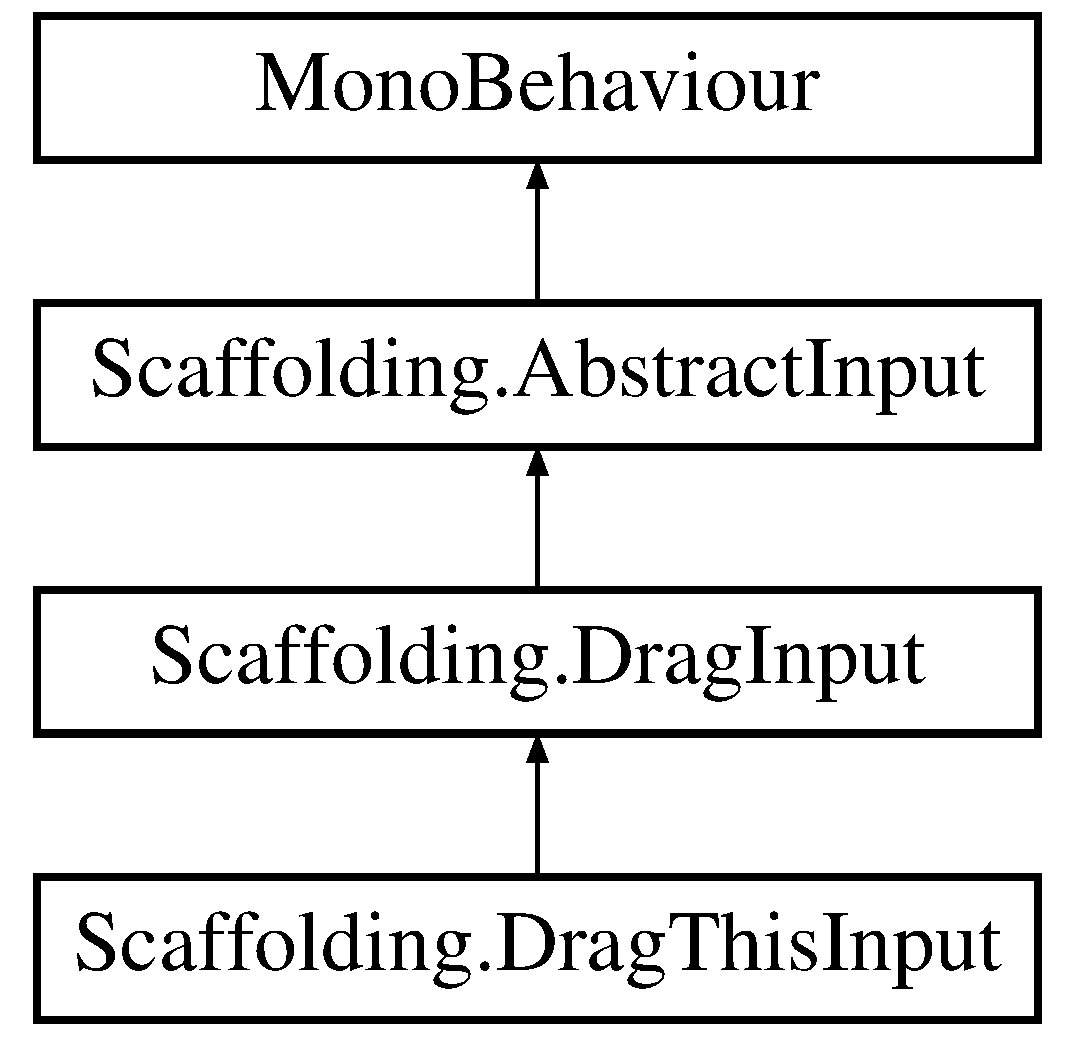
\includegraphics[height=4.000000cm]{class_scaffolding_1_1_drag_this_input}
\end{center}
\end{figure}
\subsection*{Public Member Functions}
\begin{DoxyCompactItemize}
\item 
override void \hyperlink{class_scaffolding_1_1_drag_this_input_afb612ddc8d089c8708494b57063b235d}{Setup} (\hyperlink{class_scaffolding_1_1_abstract_view}{Abstract\+View} view)
\begin{DoxyCompactList}\small\item\em Run by the view during it's setup phase. \end{DoxyCompactList}\item 
void \hyperlink{class_scaffolding_1_1_drag_this_input_a5de83a69a0b5052b9d162dcf397e5684}{Handle\+Dragged\+Callback} (Vector3 delta)
\begin{DoxyCompactList}\small\item\em Handles the dragged callback. \end{DoxyCompactList}\item 
override void \hyperlink{class_scaffolding_1_1_drag_this_input_a09639007081a6fee7bb7141ec5fa32a5}{Handle\+Event\+Pressed} (\hyperlink{class_scaffolding_1_1_input_tracker}{Input\+Tracker} tracker)
\begin{DoxyCompactList}\small\item\em Event\+Pressed, dispatched by Scaffoldings \hyperlink{class_scaffolding_1_1_input_manager}{Input\+Manager} Passes through a \hyperlink{class_scaffolding_1_1_input_tracker}{Input\+Tracker} of the current touch. \end{DoxyCompactList}\item 
override void \hyperlink{class_scaffolding_1_1_drag_this_input_a9da2ff31ce625e9880e6f47cd8617c6a}{Handle\+Event\+Released} (\hyperlink{class_scaffolding_1_1_input_tracker}{Input\+Tracker} tracker)
\begin{DoxyCompactList}\small\item\em Event\+Released, dispatched by Scaffoldings \hyperlink{class_scaffolding_1_1_input_manager}{Input\+Manager} Passes through a \hyperlink{class_scaffolding_1_1_input_tracker}{Input\+Tracker} of the current touch. \end{DoxyCompactList}\end{DoxyCompactItemize}
\subsection*{Public Attributes}
\begin{DoxyCompactItemize}
\item 
\hypertarget{class_scaffolding_1_1_drag_this_input_a5b8cb43b5f174f58c7098642fda90dcc}{string {\bfseries input\+Camera}}\label{class_scaffolding_1_1_drag_this_input_a5b8cb43b5f174f58c7098642fda90dcc}

\item 
\hypertarget{class_scaffolding_1_1_drag_this_input_a6ce7f9342173a57e81b666fdd3162c8f}{int {\bfseries input\+Camera\+Index}}\label{class_scaffolding_1_1_drag_this_input_a6ce7f9342173a57e81b666fdd3162c8f}

\item 
\hypertarget{class_scaffolding_1_1_drag_this_input_a955fd31f5d266ed13258c695c323ef7e}{int {\bfseries input\+Camera\+Length}}\label{class_scaffolding_1_1_drag_this_input_a955fd31f5d266ed13258c695c323ef7e}

\item 
\hypertarget{class_scaffolding_1_1_drag_this_input_a923518138b1f4ab3842f44db144f6d22}{int {\bfseries axis\+Drop\+Down\+Index}}\label{class_scaffolding_1_1_drag_this_input_a923518138b1f4ab3842f44db144f6d22}

\end{DoxyCompactItemize}
\subsection*{Additional Inherited Members}


\subsection{Detailed Description}
\hyperlink{class_scaffolding_1_1_drag_this_input}{Drag\+This\+Input} attaches to a gameobject as a quick solution to get something draggable. Extends \hyperlink{class_scaffolding_1_1_abstract_input}{Abstract\+Input} so falls under the same rules as other inputs in regards to views. E.\+g colliders get disabled during On\+Show\+Start and On\+Hide\+Start phases. 



\subsection{Member Function Documentation}
\hypertarget{class_scaffolding_1_1_drag_this_input_a5de83a69a0b5052b9d162dcf397e5684}{\index{Scaffolding\+::\+Drag\+This\+Input@{Scaffolding\+::\+Drag\+This\+Input}!Handle\+Dragged\+Callback@{Handle\+Dragged\+Callback}}
\index{Handle\+Dragged\+Callback@{Handle\+Dragged\+Callback}!Scaffolding\+::\+Drag\+This\+Input@{Scaffolding\+::\+Drag\+This\+Input}}
\subsubsection[{Handle\+Dragged\+Callback}]{\setlength{\rightskip}{0pt plus 5cm}void Scaffolding.\+Drag\+This\+Input.\+Handle\+Dragged\+Callback (
\begin{DoxyParamCaption}
\item[{Vector3}]{delta}
\end{DoxyParamCaption}
)}}\label{class_scaffolding_1_1_drag_this_input_a5de83a69a0b5052b9d162dcf397e5684}


Handles the dragged callback. 


\begin{DoxyParams}{Parameters}
{\em delta} & Delta.\\
\hline
\end{DoxyParams}
\hypertarget{class_scaffolding_1_1_drag_this_input_a09639007081a6fee7bb7141ec5fa32a5}{\index{Scaffolding\+::\+Drag\+This\+Input@{Scaffolding\+::\+Drag\+This\+Input}!Handle\+Event\+Pressed@{Handle\+Event\+Pressed}}
\index{Handle\+Event\+Pressed@{Handle\+Event\+Pressed}!Scaffolding\+::\+Drag\+This\+Input@{Scaffolding\+::\+Drag\+This\+Input}}
\subsubsection[{Handle\+Event\+Pressed}]{\setlength{\rightskip}{0pt plus 5cm}override void Scaffolding.\+Drag\+This\+Input.\+Handle\+Event\+Pressed (
\begin{DoxyParamCaption}
\item[{{\bf Input\+Tracker}}]{tracker}
\end{DoxyParamCaption}
)\hspace{0.3cm}{\ttfamily [virtual]}}}\label{class_scaffolding_1_1_drag_this_input_a09639007081a6fee7bb7141ec5fa32a5}


Event\+Pressed, dispatched by Scaffoldings \hyperlink{class_scaffolding_1_1_input_manager}{Input\+Manager} Passes through a \hyperlink{class_scaffolding_1_1_input_tracker}{Input\+Tracker} of the current touch. 


\begin{DoxyParams}{Parameters}
{\em tracker} & Tracker.\\
\hline
\end{DoxyParams}


Reimplemented from \hyperlink{class_scaffolding_1_1_drag_input_a49561ec761c72584711384d57cb74f41}{Scaffolding.\+Drag\+Input}.

\hypertarget{class_scaffolding_1_1_drag_this_input_a9da2ff31ce625e9880e6f47cd8617c6a}{\index{Scaffolding\+::\+Drag\+This\+Input@{Scaffolding\+::\+Drag\+This\+Input}!Handle\+Event\+Released@{Handle\+Event\+Released}}
\index{Handle\+Event\+Released@{Handle\+Event\+Released}!Scaffolding\+::\+Drag\+This\+Input@{Scaffolding\+::\+Drag\+This\+Input}}
\subsubsection[{Handle\+Event\+Released}]{\setlength{\rightskip}{0pt plus 5cm}override void Scaffolding.\+Drag\+This\+Input.\+Handle\+Event\+Released (
\begin{DoxyParamCaption}
\item[{{\bf Input\+Tracker}}]{tracker}
\end{DoxyParamCaption}
)\hspace{0.3cm}{\ttfamily [virtual]}}}\label{class_scaffolding_1_1_drag_this_input_a9da2ff31ce625e9880e6f47cd8617c6a}


Event\+Released, dispatched by Scaffoldings \hyperlink{class_scaffolding_1_1_input_manager}{Input\+Manager} Passes through a \hyperlink{class_scaffolding_1_1_input_tracker}{Input\+Tracker} of the current touch. 


\begin{DoxyParams}{Parameters}
{\em tracker} & Tracker.\\
\hline
\end{DoxyParams}


Reimplemented from \hyperlink{class_scaffolding_1_1_drag_input_ab50a7059961c803e39e3ce9ffb0945d7}{Scaffolding.\+Drag\+Input}.

\hypertarget{class_scaffolding_1_1_drag_this_input_afb612ddc8d089c8708494b57063b235d}{\index{Scaffolding\+::\+Drag\+This\+Input@{Scaffolding\+::\+Drag\+This\+Input}!Setup@{Setup}}
\index{Setup@{Setup}!Scaffolding\+::\+Drag\+This\+Input@{Scaffolding\+::\+Drag\+This\+Input}}
\subsubsection[{Setup}]{\setlength{\rightskip}{0pt plus 5cm}override void Scaffolding.\+Drag\+This\+Input.\+Setup (
\begin{DoxyParamCaption}
\item[{{\bf Abstract\+View}}]{view}
\end{DoxyParamCaption}
)\hspace{0.3cm}{\ttfamily [virtual]}}}\label{class_scaffolding_1_1_drag_this_input_afb612ddc8d089c8708494b57063b235d}


Run by the view during it's setup phase. 


\begin{DoxyParams}{Parameters}
{\em view} & View.\\
\hline
\end{DoxyParams}


Reimplemented from \hyperlink{class_scaffolding_1_1_abstract_input_a598859c6342920d2b0c985310e6e9476}{Scaffolding.\+Abstract\+Input}.



The documentation for this class was generated from the following file\+:\begin{DoxyCompactItemize}
\item 
Input/\+Items/Drag\+This\+Input.\+cs\end{DoxyCompactItemize}

\hypertarget{class_scaffolding_1_1_input_manager}{\section{Scaffolding.\-Input\-Manager Class Reference}
\label{class_scaffolding_1_1_input_manager}\index{Scaffolding.\-Input\-Manager@{Scaffolding.\-Input\-Manager}}
}


Scaffoldings \hyperlink{class_scaffolding_1_1_input_manager}{Input\-Manager} is a multitouch input manager that looks after all the inputs used within scaffoldings \hyperlink{class_scaffolding_1_1_abstract_input}{Abstract\-Input} class. \hyperlink{namespace_scaffolding}{Scaffolding} is multitouch from the core and built upon the idea that you should be able to place your whole hand on the screen and still use buttons.  


Inheritance diagram for Scaffolding.\-Input\-Manager\-:\begin{figure}[H]
\begin{center}
\leavevmode
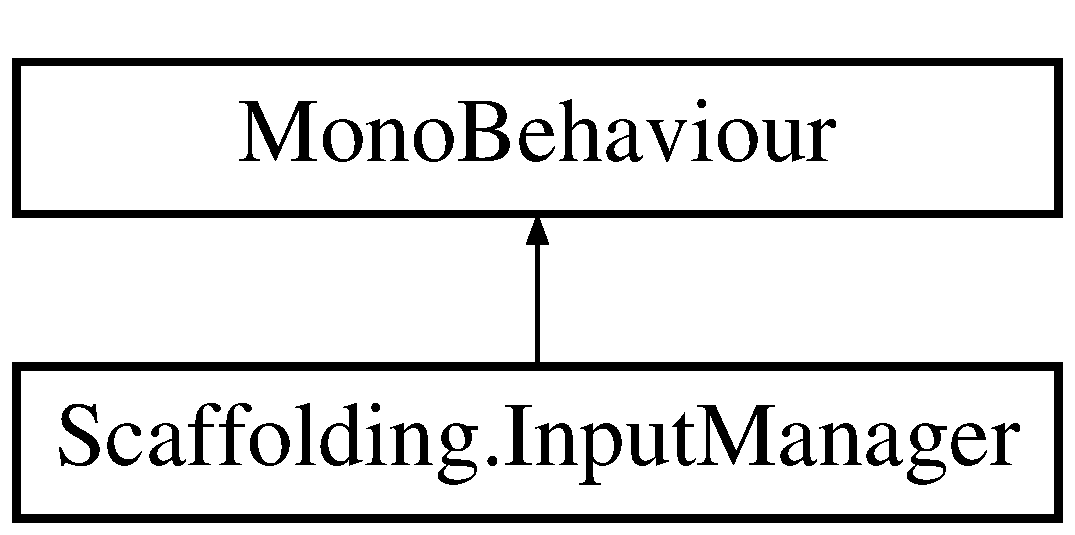
\includegraphics[height=2.000000cm]{class_scaffolding_1_1_input_manager}
\end{center}
\end{figure}
\subsection*{Public Member Functions}
\begin{DoxyCompactItemize}
\item 
\hypertarget{class_scaffolding_1_1_input_manager_ae7622b2ff061b41fef5b7949cef8804b}{delegate void {\bfseries Input\-Event} (\hyperlink{class_scaffolding_1_1_input_tracker}{Input\-Tracker} tracker)}\label{class_scaffolding_1_1_input_manager_ae7622b2ff061b41fef5b7949cef8804b}

\item 
\hypertarget{class_scaffolding_1_1_input_manager_a5f228d24dde2dfd00bf06d20631d2467}{delegate void {\bfseries Input\-Event\-Delta} (Vector3 position)}\label{class_scaffolding_1_1_input_manager_a5f228d24dde2dfd00bf06d20631d2467}

\end{DoxyCompactItemize}
\subsection*{Events}
\begin{DoxyCompactItemize}
\item 
\hypertarget{class_scaffolding_1_1_input_manager_a0cd2afadd2f9bf461269497b0ba988ef}{Input\-Event {\bfseries Event\-Pressed}}\label{class_scaffolding_1_1_input_manager_a0cd2afadd2f9bf461269497b0ba988ef}

\item 
\hypertarget{class_scaffolding_1_1_input_manager_a2ea3e35f371d9777d16174216a156ba9}{Input\-Event {\bfseries Event\-Released}}\label{class_scaffolding_1_1_input_manager_a2ea3e35f371d9777d16174216a156ba9}

\item 
\hypertarget{class_scaffolding_1_1_input_manager_af97450c838114a179c136de954764955}{Input\-Event {\bfseries Event\-Dragged}}\label{class_scaffolding_1_1_input_manager_af97450c838114a179c136de954764955}

\item 
\hypertarget{class_scaffolding_1_1_input_manager_a9317d8d6bb537c1614c925390c1442a5}{Input\-Event\-Delta {\bfseries Event\-Dragged\-Delta}}\label{class_scaffolding_1_1_input_manager_a9317d8d6bb537c1614c925390c1442a5}

\end{DoxyCompactItemize}


\subsection{Detailed Description}
Scaffoldings \hyperlink{class_scaffolding_1_1_input_manager}{Input\-Manager} is a multitouch input manager that looks after all the inputs used within scaffoldings \hyperlink{class_scaffolding_1_1_abstract_input}{Abstract\-Input} class. \hyperlink{namespace_scaffolding}{Scaffolding} is multitouch from the core and built upon the idea that you should be able to place your whole hand on the screen and still use buttons. 



The documentation for this class was generated from the following file\-:\begin{DoxyCompactItemize}
\item 
Input/Input\-Manager.\-cs\end{DoxyCompactItemize}

\hypertarget{class_scaffolding_1_1_input_tracker}{\section{Scaffolding.\-Input\-Tracker Class Reference}
\label{class_scaffolding_1_1_input_tracker}\index{Scaffolding.\-Input\-Tracker@{Scaffolding.\-Input\-Tracker}}
}


Input tracker, tracks every finger or mouse press that happens within Scaffoldings views.  


\subsection*{Public Member Functions}
\begin{DoxyCompactItemize}
\item 
\hyperlink{class_scaffolding_1_1_input_tracker_aa20fb06b3415f79e7d79c9cbfabc0a99}{Input\-Tracker} (int id, Vector3 \hyperlink{class_scaffolding_1_1_input_tracker_ab29b6a8291f5f49035544a3c6e592be0}{position})
\begin{DoxyCompactList}\small\item\em Initializes a new instance of the \hyperlink{class_scaffolding_1_1_input_tracker}{Scaffolding.\-Input\-Tracker} class. \end{DoxyCompactList}\item 
void \hyperlink{class_scaffolding_1_1_input_tracker_aedce3144315d02e9713c7fddacafe5aa}{Update\-Tracker} (Vector3 \hyperlink{class_scaffolding_1_1_input_tracker_ab29b6a8291f5f49035544a3c6e592be0}{position})
\begin{DoxyCompactList}\small\item\em Update the specified position. \end{DoxyCompactList}\item 
void \hyperlink{class_scaffolding_1_1_input_tracker_afa1ed7b953c814e9b45a6348c6d08c85}{Set\-New\-Velocity\-Data} (float time, Vector3 \hyperlink{class_scaffolding_1_1_input_tracker_ab29b6a8291f5f49035544a3c6e592be0}{position})
\begin{DoxyCompactList}\small\item\em Sets the new velocity data. \end{DoxyCompactList}\item 
void \hyperlink{class_scaffolding_1_1_input_tracker_a38e432bbd719c51f738311b153d6df70}{Kill\-Tracker} ()
\begin{DoxyCompactList}\small\item\em Clean this instance. \end{DoxyCompactList}\item 
virtual void \hyperlink{class_scaffolding_1_1_input_tracker_a354f0c69074700a14d7d969d9e6b18e4}{Start\-Tracking} ()
\begin{DoxyCompactList}\small\item\em Start tracking the input \end{DoxyCompactList}\item 
virtual void \hyperlink{class_scaffolding_1_1_input_tracker_a2381c906d5c7c84cb8fad33ad95c7386}{Stop\-Tracking} ()
\begin{DoxyCompactList}\small\item\em Stop tracking the input \end{DoxyCompactList}\end{DoxyCompactItemize}
\subsection*{Properties}
\begin{DoxyCompactItemize}
\item 
int \hyperlink{class_scaffolding_1_1_input_tracker_a2ea83b7d3578473eaddc1360739b48e7}{finger\-Id}\hspace{0.3cm}{\ttfamily  \mbox{[}get\mbox{]}}
\begin{DoxyCompactList}\small\item\em Gets the finger identifier. \end{DoxyCompactList}\item 
bool \hyperlink{class_scaffolding_1_1_input_tracker_ac490c7f5cc792230aa3ca2fd87fb43b4}{alive}\hspace{0.3cm}{\ttfamily  \mbox{[}get\mbox{]}}
\begin{DoxyCompactList}\small\item\em Gets a value indicating whether this \hyperlink{class_scaffolding_1_1_input_tracker}{Scaffolding.\-Input\-Tracker} is dirty. \end{DoxyCompactList}\item 
Vector3 \hyperlink{class_scaffolding_1_1_input_tracker_ab29b6a8291f5f49035544a3c6e592be0}{position}\hspace{0.3cm}{\ttfamily  \mbox{[}get\mbox{]}}
\begin{DoxyCompactList}\small\item\em Gets the current position of the input. \end{DoxyCompactList}\item 
Vector3 \hyperlink{class_scaffolding_1_1_input_tracker_a7f6ba8cef62bec4066f132a3d0d1f7c1}{delta\-Position}\hspace{0.3cm}{\ttfamily  \mbox{[}get\mbox{]}}
\begin{DoxyCompactList}\small\item\em Gets the delta position. \end{DoxyCompactList}\item 
Vector2 \hyperlink{class_scaffolding_1_1_input_tracker_a1cca0ea0d1202267e88f7a88f511d2c5}{velocity}\hspace{0.3cm}{\ttfamily  \mbox{[}get\mbox{]}}
\begin{DoxyCompactList}\small\item\em Gets the velocity. \end{DoxyCompactList}\end{DoxyCompactItemize}


\subsection{Detailed Description}
Input tracker, tracks every finger or mouse press that happens within Scaffoldings views. 



\subsection{Constructor \& Destructor Documentation}
\hypertarget{class_scaffolding_1_1_input_tracker_aa20fb06b3415f79e7d79c9cbfabc0a99}{\index{Scaffolding\-::\-Input\-Tracker@{Scaffolding\-::\-Input\-Tracker}!Input\-Tracker@{Input\-Tracker}}
\index{Input\-Tracker@{Input\-Tracker}!Scaffolding::InputTracker@{Scaffolding\-::\-Input\-Tracker}}
\subsubsection[{Input\-Tracker}]{\setlength{\rightskip}{0pt plus 5cm}Scaffolding.\-Input\-Tracker.\-Input\-Tracker (
\begin{DoxyParamCaption}
\item[{int}]{id, }
\item[{Vector3}]{position}
\end{DoxyParamCaption}
)}}\label{class_scaffolding_1_1_input_tracker_aa20fb06b3415f79e7d79c9cbfabc0a99}


Initializes a new instance of the \hyperlink{class_scaffolding_1_1_input_tracker}{Scaffolding.\-Input\-Tracker} class. 


\begin{DoxyParams}{Parameters}
{\em id} & Identifier.\\
\hline
{\em position} & Position.\\
\hline
\end{DoxyParams}


\subsection{Member Function Documentation}
\hypertarget{class_scaffolding_1_1_input_tracker_a38e432bbd719c51f738311b153d6df70}{\index{Scaffolding\-::\-Input\-Tracker@{Scaffolding\-::\-Input\-Tracker}!Kill\-Tracker@{Kill\-Tracker}}
\index{Kill\-Tracker@{Kill\-Tracker}!Scaffolding::InputTracker@{Scaffolding\-::\-Input\-Tracker}}
\subsubsection[{Kill\-Tracker}]{\setlength{\rightskip}{0pt plus 5cm}void Scaffolding.\-Input\-Tracker.\-Kill\-Tracker (
\begin{DoxyParamCaption}
{}
\end{DoxyParamCaption}
)}}\label{class_scaffolding_1_1_input_tracker_a38e432bbd719c51f738311b153d6df70}


Clean this instance. 

\hypertarget{class_scaffolding_1_1_input_tracker_afa1ed7b953c814e9b45a6348c6d08c85}{\index{Scaffolding\-::\-Input\-Tracker@{Scaffolding\-::\-Input\-Tracker}!Set\-New\-Velocity\-Data@{Set\-New\-Velocity\-Data}}
\index{Set\-New\-Velocity\-Data@{Set\-New\-Velocity\-Data}!Scaffolding::InputTracker@{Scaffolding\-::\-Input\-Tracker}}
\subsubsection[{Set\-New\-Velocity\-Data}]{\setlength{\rightskip}{0pt plus 5cm}void Scaffolding.\-Input\-Tracker.\-Set\-New\-Velocity\-Data (
\begin{DoxyParamCaption}
\item[{float}]{time, }
\item[{Vector3}]{position}
\end{DoxyParamCaption}
)}}\label{class_scaffolding_1_1_input_tracker_afa1ed7b953c814e9b45a6348c6d08c85}


Sets the new velocity data. 


\begin{DoxyParams}{Parameters}
{\em time} & Time.\\
\hline
{\em position} & Position.\\
\hline
\end{DoxyParams}
\hypertarget{class_scaffolding_1_1_input_tracker_a354f0c69074700a14d7d969d9e6b18e4}{\index{Scaffolding\-::\-Input\-Tracker@{Scaffolding\-::\-Input\-Tracker}!Start\-Tracking@{Start\-Tracking}}
\index{Start\-Tracking@{Start\-Tracking}!Scaffolding::InputTracker@{Scaffolding\-::\-Input\-Tracker}}
\subsubsection[{Start\-Tracking}]{\setlength{\rightskip}{0pt plus 5cm}virtual void Scaffolding.\-Input\-Tracker.\-Start\-Tracking (
\begin{DoxyParamCaption}
{}
\end{DoxyParamCaption}
)\hspace{0.3cm}{\ttfamily [virtual]}}}\label{class_scaffolding_1_1_input_tracker_a354f0c69074700a14d7d969d9e6b18e4}


Start tracking the input 

\hypertarget{class_scaffolding_1_1_input_tracker_a2381c906d5c7c84cb8fad33ad95c7386}{\index{Scaffolding\-::\-Input\-Tracker@{Scaffolding\-::\-Input\-Tracker}!Stop\-Tracking@{Stop\-Tracking}}
\index{Stop\-Tracking@{Stop\-Tracking}!Scaffolding::InputTracker@{Scaffolding\-::\-Input\-Tracker}}
\subsubsection[{Stop\-Tracking}]{\setlength{\rightskip}{0pt plus 5cm}virtual void Scaffolding.\-Input\-Tracker.\-Stop\-Tracking (
\begin{DoxyParamCaption}
{}
\end{DoxyParamCaption}
)\hspace{0.3cm}{\ttfamily [virtual]}}}\label{class_scaffolding_1_1_input_tracker_a2381c906d5c7c84cb8fad33ad95c7386}


Stop tracking the input 

\hypertarget{class_scaffolding_1_1_input_tracker_aedce3144315d02e9713c7fddacafe5aa}{\index{Scaffolding\-::\-Input\-Tracker@{Scaffolding\-::\-Input\-Tracker}!Update\-Tracker@{Update\-Tracker}}
\index{Update\-Tracker@{Update\-Tracker}!Scaffolding::InputTracker@{Scaffolding\-::\-Input\-Tracker}}
\subsubsection[{Update\-Tracker}]{\setlength{\rightskip}{0pt plus 5cm}void Scaffolding.\-Input\-Tracker.\-Update\-Tracker (
\begin{DoxyParamCaption}
\item[{Vector3}]{position}
\end{DoxyParamCaption}
)}}\label{class_scaffolding_1_1_input_tracker_aedce3144315d02e9713c7fddacafe5aa}


Update the specified position. 


\begin{DoxyParams}{Parameters}
{\em position} & Position.\\
\hline
\end{DoxyParams}


\subsection{Property Documentation}
\hypertarget{class_scaffolding_1_1_input_tracker_ac490c7f5cc792230aa3ca2fd87fb43b4}{\index{Scaffolding\-::\-Input\-Tracker@{Scaffolding\-::\-Input\-Tracker}!alive@{alive}}
\index{alive@{alive}!Scaffolding::InputTracker@{Scaffolding\-::\-Input\-Tracker}}
\subsubsection[{alive}]{\setlength{\rightskip}{0pt plus 5cm}bool Scaffolding.\-Input\-Tracker.\-alive\hspace{0.3cm}{\ttfamily [get]}}}\label{class_scaffolding_1_1_input_tracker_ac490c7f5cc792230aa3ca2fd87fb43b4}


Gets a value indicating whether this \hyperlink{class_scaffolding_1_1_input_tracker}{Scaffolding.\-Input\-Tracker} is dirty. 

{\ttfamily true} if is dirty; otherwise, {\ttfamily false}.\hypertarget{class_scaffolding_1_1_input_tracker_a7f6ba8cef62bec4066f132a3d0d1f7c1}{\index{Scaffolding\-::\-Input\-Tracker@{Scaffolding\-::\-Input\-Tracker}!delta\-Position@{delta\-Position}}
\index{delta\-Position@{delta\-Position}!Scaffolding::InputTracker@{Scaffolding\-::\-Input\-Tracker}}
\subsubsection[{delta\-Position}]{\setlength{\rightskip}{0pt plus 5cm}Vector3 Scaffolding.\-Input\-Tracker.\-delta\-Position\hspace{0.3cm}{\ttfamily [get]}}}\label{class_scaffolding_1_1_input_tracker_a7f6ba8cef62bec4066f132a3d0d1f7c1}


Gets the delta position. 

The delta position.\hypertarget{class_scaffolding_1_1_input_tracker_a2ea83b7d3578473eaddc1360739b48e7}{\index{Scaffolding\-::\-Input\-Tracker@{Scaffolding\-::\-Input\-Tracker}!finger\-Id@{finger\-Id}}
\index{finger\-Id@{finger\-Id}!Scaffolding::InputTracker@{Scaffolding\-::\-Input\-Tracker}}
\subsubsection[{finger\-Id}]{\setlength{\rightskip}{0pt plus 5cm}int Scaffolding.\-Input\-Tracker.\-finger\-Id\hspace{0.3cm}{\ttfamily [get]}}}\label{class_scaffolding_1_1_input_tracker_a2ea83b7d3578473eaddc1360739b48e7}


Gets the finger identifier. 

The finger identifier.\hypertarget{class_scaffolding_1_1_input_tracker_ab29b6a8291f5f49035544a3c6e592be0}{\index{Scaffolding\-::\-Input\-Tracker@{Scaffolding\-::\-Input\-Tracker}!position@{position}}
\index{position@{position}!Scaffolding::InputTracker@{Scaffolding\-::\-Input\-Tracker}}
\subsubsection[{position}]{\setlength{\rightskip}{0pt plus 5cm}Vector3 Scaffolding.\-Input\-Tracker.\-position\hspace{0.3cm}{\ttfamily [get]}}}\label{class_scaffolding_1_1_input_tracker_ab29b6a8291f5f49035544a3c6e592be0}


Gets the current position of the input. 

The position.\hypertarget{class_scaffolding_1_1_input_tracker_a1cca0ea0d1202267e88f7a88f511d2c5}{\index{Scaffolding\-::\-Input\-Tracker@{Scaffolding\-::\-Input\-Tracker}!velocity@{velocity}}
\index{velocity@{velocity}!Scaffolding::InputTracker@{Scaffolding\-::\-Input\-Tracker}}
\subsubsection[{velocity}]{\setlength{\rightskip}{0pt plus 5cm}Vector2 Scaffolding.\-Input\-Tracker.\-velocity\hspace{0.3cm}{\ttfamily [get]}}}\label{class_scaffolding_1_1_input_tracker_a1cca0ea0d1202267e88f7a88f511d2c5}


Gets the velocity. 

The velocity.

The documentation for this class was generated from the following file\-:\begin{DoxyCompactItemize}
\item 
Input/Input\-Tracker.\-cs\end{DoxyCompactItemize}

\hypertarget{interface_scaffolding_1_1_i_requestable}{\section{Scaffolding.\+I\+Requestable Interface Reference}
\label{interface_scaffolding_1_1_i_requestable}\index{Scaffolding.\+I\+Requestable@{Scaffolding.\+I\+Requestable}}
}
Inheritance diagram for Scaffolding.\+I\+Requestable\+:\begin{figure}[H]
\begin{center}
\leavevmode
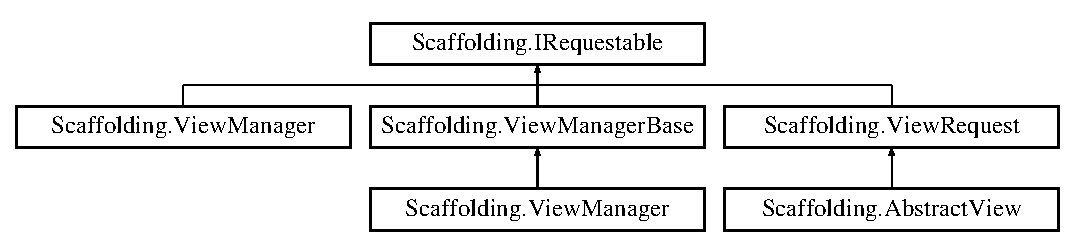
\includegraphics[height=2.871795cm]{interface_scaffolding_1_1_i_requestable}
\end{center}
\end{figure}
\subsection*{Public Member Functions}
\begin{DoxyCompactItemize}
\item 
\hypertarget{interface_scaffolding_1_1_i_requestable_ace2161c2dae06f16ff059aac5a0507fc}{void {\bfseries Request\+Overlay$<$ T $>$} ()}\label{interface_scaffolding_1_1_i_requestable_ace2161c2dae06f16ff059aac5a0507fc}

\item 
\hypertarget{interface_scaffolding_1_1_i_requestable_abda3fb68ddbe85d6157ce22b86f9ebaa}{void {\bfseries Request\+Overlay} (Type type)}\label{interface_scaffolding_1_1_i_requestable_abda3fb68ddbe85d6157ce22b86f9ebaa}

\item 
\hypertarget{interface_scaffolding_1_1_i_requestable_acba0a4773ac0db529ecede3148030f3f}{void {\bfseries Request\+Overlay\+Close$<$ T $>$} ()}\label{interface_scaffolding_1_1_i_requestable_acba0a4773ac0db529ecede3148030f3f}

\item 
\hypertarget{interface_scaffolding_1_1_i_requestable_a5cb3fd2ce89b2534e11ca9cb50419e38}{void {\bfseries Request\+Overlay\+Close} (Type type)}\label{interface_scaffolding_1_1_i_requestable_a5cb3fd2ce89b2534e11ca9cb50419e38}

\item 
\hypertarget{interface_scaffolding_1_1_i_requestable_a311188c70a3fc0263445efaf53ac32e9}{void {\bfseries Request\+Overlay\+Force\+Close$<$ T $>$} ()}\label{interface_scaffolding_1_1_i_requestable_a311188c70a3fc0263445efaf53ac32e9}

\item 
\hypertarget{interface_scaffolding_1_1_i_requestable_a94199ff3b82b0e7bb44d469c1faad5bc}{void {\bfseries Request\+Overlay\+Force\+Close} (Type type)}\label{interface_scaffolding_1_1_i_requestable_a94199ff3b82b0e7bb44d469c1faad5bc}

\item 
\hypertarget{interface_scaffolding_1_1_i_requestable_ace3bf254580709e3df046a70c4c101fa}{void {\bfseries Request\+View$<$ T $>$} ()}\label{interface_scaffolding_1_1_i_requestable_ace3bf254580709e3df046a70c4c101fa}

\item 
\hypertarget{interface_scaffolding_1_1_i_requestable_a8cbc0942794c6d8162e641d995038cc9}{void {\bfseries Request\+View} (Type type)}\label{interface_scaffolding_1_1_i_requestable_a8cbc0942794c6d8162e641d995038cc9}

\item 
\hypertarget{interface_scaffolding_1_1_i_requestable_a7bd29fd5ec68858da4c8626b93d7fb3a}{void {\bfseries Request\+Force\+Reopen\+View$<$ T $>$} ()}\label{interface_scaffolding_1_1_i_requestable_a7bd29fd5ec68858da4c8626b93d7fb3a}

\item 
\hypertarget{interface_scaffolding_1_1_i_requestable_aea438ab1307dc5ffee48379f6beb17f8}{void {\bfseries Request\+Force\+Reopen\+View} (Type type)}\label{interface_scaffolding_1_1_i_requestable_aea438ab1307dc5ffee48379f6beb17f8}

\item 
\hypertarget{interface_scaffolding_1_1_i_requestable_ab8c48103df46a4ff2ee11832a4e299cc}{void {\bfseries Request\+View\+With\+Loading\+Overlay$<$ T, L $>$} ()}\label{interface_scaffolding_1_1_i_requestable_ab8c48103df46a4ff2ee11832a4e299cc}

\item 
\hypertarget{interface_scaffolding_1_1_i_requestable_a2b9c62403a1938d6fd638b3d300cc834}{void {\bfseries Request\+View\+With\+Loading\+Overlay} (Type type, Type loading\+Type)}\label{interface_scaffolding_1_1_i_requestable_a2b9c62403a1938d6fd638b3d300cc834}

\end{DoxyCompactItemize}


The documentation for this interface was generated from the following file\+:\begin{DoxyCompactItemize}
\item 
Views/I\+Requestable.\+cs\end{DoxyCompactItemize}

\hypertarget{class_scaffolding_1_1_pinch_input}{\section{Scaffolding.\+Pinch\+Input Class Reference}
\label{class_scaffolding_1_1_pinch_input}\index{Scaffolding.\+Pinch\+Input@{Scaffolding.\+Pinch\+Input}}
}


Pinch input is largely a touch input based class. It replicates the pinch gesture, and dispatches a callback while pinching.  


Inheritance diagram for Scaffolding.\+Pinch\+Input\+:\begin{figure}[H]
\begin{center}
\leavevmode
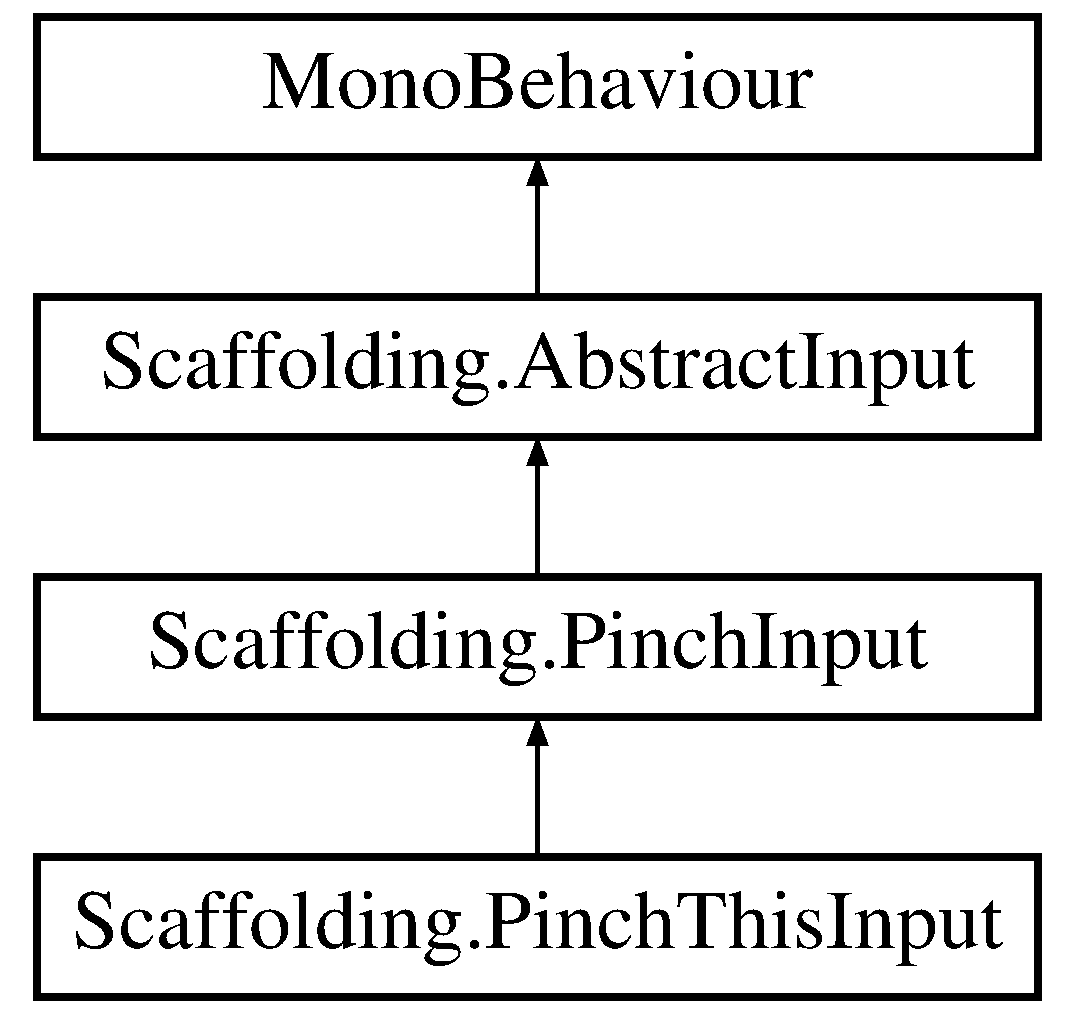
\includegraphics[height=4.000000cm]{class_scaffolding_1_1_pinch_input}
\end{center}
\end{figure}
\subsection*{Public Member Functions}
\begin{DoxyCompactItemize}
\item 
override void \hyperlink{class_scaffolding_1_1_pinch_input_aa6687d25d10c2f4e7106641e0647af35}{Setup} (\hyperlink{class_scaffolding_1_1_abstract_view}{Abstract\+View} view)
\begin{DoxyCompactList}\small\item\em Run by the view during it's setup phase. \end{DoxyCompactList}\item 
override void \hyperlink{class_scaffolding_1_1_pinch_input_a5849a64ba0a49d679e4a57fc28fe3f7a}{Cleanup} ()
\begin{DoxyCompactList}\small\item\em The inputs clean up phase. \end{DoxyCompactList}\item 
void \hyperlink{class_scaffolding_1_1_pinch_input_acaa10def18626148f344a8a50bdca22b}{Register\+Pinch\+Callback} (Action$<$ float $>$ callback)
\begin{DoxyCompactList}\small\item\em Registers the pinch callback. \end{DoxyCompactList}\item 
override void \hyperlink{class_scaffolding_1_1_pinch_input_aea53be8e94bef95c8373dd05639eaa41}{Handle\+Event\+Pressed} (\hyperlink{class_scaffolding_1_1_input_tracker}{Input\+Tracker} tracker)
\begin{DoxyCompactList}\small\item\em Event\+Pressed, dispatched by Scaffoldings \hyperlink{class_scaffolding_1_1_input_manager}{Input\+Manager} Passes through a \hyperlink{class_scaffolding_1_1_input_tracker}{Input\+Tracker} of the current touch. \end{DoxyCompactList}\item 
override void \hyperlink{class_scaffolding_1_1_pinch_input_a865f0201d2b7930241711abb68a7341d}{Handle\+Event\+Dragged} (\hyperlink{class_scaffolding_1_1_input_tracker}{Input\+Tracker} tracker)
\begin{DoxyCompactList}\small\item\em Event\+Dragged, dispatched by the Scaffoldings \hyperlink{class_scaffolding_1_1_input_manager}{Input\+Manager} Passes through an \hyperlink{class_scaffolding_1_1_input_tracker}{Input\+Tracker} of the current touch. \end{DoxyCompactList}\item 
override void \hyperlink{class_scaffolding_1_1_pinch_input_ad7e6fa3689011526acda972b7f6f4aa8}{Handle\+Event\+Released} (\hyperlink{class_scaffolding_1_1_input_tracker}{Input\+Tracker} tracker)
\begin{DoxyCompactList}\small\item\em Event\+Released, dispatched by the Scaffoldings \hyperlink{class_scaffolding_1_1_input_manager}{Input\+Manager} Passes through a \hyperlink{class_scaffolding_1_1_input_tracker}{Input\+Tracker} of the current touch. \end{DoxyCompactList}\end{DoxyCompactItemize}


\subsection{Detailed Description}
Pinch input is largely a touch input based class. It replicates the pinch gesture, and dispatches a callback while pinching. 



\subsection{Member Function Documentation}
\hypertarget{class_scaffolding_1_1_pinch_input_a5849a64ba0a49d679e4a57fc28fe3f7a}{\index{Scaffolding\+::\+Pinch\+Input@{Scaffolding\+::\+Pinch\+Input}!Cleanup@{Cleanup}}
\index{Cleanup@{Cleanup}!Scaffolding\+::\+Pinch\+Input@{Scaffolding\+::\+Pinch\+Input}}
\subsubsection[{Cleanup}]{\setlength{\rightskip}{0pt plus 5cm}override void Scaffolding.\+Pinch\+Input.\+Cleanup (
\begin{DoxyParamCaption}
{}
\end{DoxyParamCaption}
)\hspace{0.3cm}{\ttfamily [virtual]}}}\label{class_scaffolding_1_1_pinch_input_a5849a64ba0a49d679e4a57fc28fe3f7a}


The inputs clean up phase. 



Reimplemented from \hyperlink{class_scaffolding_1_1_abstract_input_ab179ae99e76c6c934a0dcba4fc195e68}{Scaffolding.\+Abstract\+Input}.

\hypertarget{class_scaffolding_1_1_pinch_input_a865f0201d2b7930241711abb68a7341d}{\index{Scaffolding\+::\+Pinch\+Input@{Scaffolding\+::\+Pinch\+Input}!Handle\+Event\+Dragged@{Handle\+Event\+Dragged}}
\index{Handle\+Event\+Dragged@{Handle\+Event\+Dragged}!Scaffolding\+::\+Pinch\+Input@{Scaffolding\+::\+Pinch\+Input}}
\subsubsection[{Handle\+Event\+Dragged}]{\setlength{\rightskip}{0pt plus 5cm}override void Scaffolding.\+Pinch\+Input.\+Handle\+Event\+Dragged (
\begin{DoxyParamCaption}
\item[{{\bf Input\+Tracker}}]{tracker}
\end{DoxyParamCaption}
)\hspace{0.3cm}{\ttfamily [virtual]}}}\label{class_scaffolding_1_1_pinch_input_a865f0201d2b7930241711abb68a7341d}


Event\+Dragged, dispatched by the Scaffoldings \hyperlink{class_scaffolding_1_1_input_manager}{Input\+Manager} Passes through an \hyperlink{class_scaffolding_1_1_input_tracker}{Input\+Tracker} of the current touch. 


\begin{DoxyParams}{Parameters}
{\em tracker} & Tracker.\\
\hline
\end{DoxyParams}


Reimplemented from \hyperlink{class_scaffolding_1_1_abstract_input_a5996b0cb611a384e527ce871b9607858}{Scaffolding.\+Abstract\+Input}.

\hypertarget{class_scaffolding_1_1_pinch_input_aea53be8e94bef95c8373dd05639eaa41}{\index{Scaffolding\+::\+Pinch\+Input@{Scaffolding\+::\+Pinch\+Input}!Handle\+Event\+Pressed@{Handle\+Event\+Pressed}}
\index{Handle\+Event\+Pressed@{Handle\+Event\+Pressed}!Scaffolding\+::\+Pinch\+Input@{Scaffolding\+::\+Pinch\+Input}}
\subsubsection[{Handle\+Event\+Pressed}]{\setlength{\rightskip}{0pt plus 5cm}override void Scaffolding.\+Pinch\+Input.\+Handle\+Event\+Pressed (
\begin{DoxyParamCaption}
\item[{{\bf Input\+Tracker}}]{tracker}
\end{DoxyParamCaption}
)\hspace{0.3cm}{\ttfamily [virtual]}}}\label{class_scaffolding_1_1_pinch_input_aea53be8e94bef95c8373dd05639eaa41}


Event\+Pressed, dispatched by Scaffoldings \hyperlink{class_scaffolding_1_1_input_manager}{Input\+Manager} Passes through a \hyperlink{class_scaffolding_1_1_input_tracker}{Input\+Tracker} of the current touch. 


\begin{DoxyParams}{Parameters}
{\em tracker} & Tracker.\\
\hline
\end{DoxyParams}


Reimplemented from \hyperlink{class_scaffolding_1_1_abstract_input_a11e83c3462719749f8281a21024e902f}{Scaffolding.\+Abstract\+Input}.



Reimplemented in \hyperlink{class_scaffolding_1_1_pinch_this_input_a00f941bc53b1847a2be7a2e61a4a9a57}{Scaffolding.\+Pinch\+This\+Input}.

\hypertarget{class_scaffolding_1_1_pinch_input_ad7e6fa3689011526acda972b7f6f4aa8}{\index{Scaffolding\+::\+Pinch\+Input@{Scaffolding\+::\+Pinch\+Input}!Handle\+Event\+Released@{Handle\+Event\+Released}}
\index{Handle\+Event\+Released@{Handle\+Event\+Released}!Scaffolding\+::\+Pinch\+Input@{Scaffolding\+::\+Pinch\+Input}}
\subsubsection[{Handle\+Event\+Released}]{\setlength{\rightskip}{0pt plus 5cm}override void Scaffolding.\+Pinch\+Input.\+Handle\+Event\+Released (
\begin{DoxyParamCaption}
\item[{{\bf Input\+Tracker}}]{tracker}
\end{DoxyParamCaption}
)\hspace{0.3cm}{\ttfamily [virtual]}}}\label{class_scaffolding_1_1_pinch_input_ad7e6fa3689011526acda972b7f6f4aa8}


Event\+Released, dispatched by the Scaffoldings \hyperlink{class_scaffolding_1_1_input_manager}{Input\+Manager} Passes through a \hyperlink{class_scaffolding_1_1_input_tracker}{Input\+Tracker} of the current touch. 


\begin{DoxyParams}{Parameters}
{\em tracker} & Tracker.\\
\hline
\end{DoxyParams}


Reimplemented from \hyperlink{class_scaffolding_1_1_abstract_input_a11854454457cd55a26f345011f4bd6bc}{Scaffolding.\+Abstract\+Input}.



Reimplemented in \hyperlink{class_scaffolding_1_1_pinch_this_input_ad9ca7c0e4b14d3d59ff06b258b4b9f7d}{Scaffolding.\+Pinch\+This\+Input}.

\hypertarget{class_scaffolding_1_1_pinch_input_acaa10def18626148f344a8a50bdca22b}{\index{Scaffolding\+::\+Pinch\+Input@{Scaffolding\+::\+Pinch\+Input}!Register\+Pinch\+Callback@{Register\+Pinch\+Callback}}
\index{Register\+Pinch\+Callback@{Register\+Pinch\+Callback}!Scaffolding\+::\+Pinch\+Input@{Scaffolding\+::\+Pinch\+Input}}
\subsubsection[{Register\+Pinch\+Callback}]{\setlength{\rightskip}{0pt plus 5cm}void Scaffolding.\+Pinch\+Input.\+Register\+Pinch\+Callback (
\begin{DoxyParamCaption}
\item[{Action$<$ float $>$}]{callback}
\end{DoxyParamCaption}
)}}\label{class_scaffolding_1_1_pinch_input_acaa10def18626148f344a8a50bdca22b}


Registers the pinch callback. 

Example\+: public void My\+Callback\+Function(float delta\+Distance) \{ //do pinch based code here... \}

\+\_\+pinch\+Input.\+Register\+Pinch\+Callback(\+My\+Callback\+Function);


\begin{DoxyParams}{Parameters}
{\em callback} & Callback.\\
\hline
\end{DoxyParams}
\hypertarget{class_scaffolding_1_1_pinch_input_aa6687d25d10c2f4e7106641e0647af35}{\index{Scaffolding\+::\+Pinch\+Input@{Scaffolding\+::\+Pinch\+Input}!Setup@{Setup}}
\index{Setup@{Setup}!Scaffolding\+::\+Pinch\+Input@{Scaffolding\+::\+Pinch\+Input}}
\subsubsection[{Setup}]{\setlength{\rightskip}{0pt plus 5cm}override void Scaffolding.\+Pinch\+Input.\+Setup (
\begin{DoxyParamCaption}
\item[{{\bf Abstract\+View}}]{view}
\end{DoxyParamCaption}
)\hspace{0.3cm}{\ttfamily [virtual]}}}\label{class_scaffolding_1_1_pinch_input_aa6687d25d10c2f4e7106641e0647af35}


Run by the view during it's setup phase. 


\begin{DoxyParams}{Parameters}
{\em view} & View.\\
\hline
\end{DoxyParams}


Reimplemented from \hyperlink{class_scaffolding_1_1_abstract_input_a598859c6342920d2b0c985310e6e9476}{Scaffolding.\+Abstract\+Input}.



Reimplemented in \hyperlink{class_scaffolding_1_1_pinch_this_input_a60b5bc5461de1286d8bd142742451dab}{Scaffolding.\+Pinch\+This\+Input}.



The documentation for this class was generated from the following file\+:\begin{DoxyCompactItemize}
\item 
Input/\+Items/Pinch\+Input.\+cs\end{DoxyCompactItemize}

\hypertarget{class_scaffolding_1_1_pinch_this_input}{\section{Scaffolding.\+Pinch\+This\+Input Class Reference}
\label{class_scaffolding_1_1_pinch_this_input}\index{Scaffolding.\+Pinch\+This\+Input@{Scaffolding.\+Pinch\+This\+Input}}
}


\hyperlink{class_scaffolding_1_1_pinch_this_input}{Pinch\+This\+Input} attaches to a gameobject as a quick solution to get something to respond to the pinch gesture. Extends \hyperlink{class_scaffolding_1_1_abstract_input}{Abstract\+Input} so falls under the same rules as other inputs in regards to views. E.\+g colliders get disabled during On\+Show\+Start and On\+Hide\+Start phases.  


Inheritance diagram for Scaffolding.\+Pinch\+This\+Input\+:\begin{figure}[H]
\begin{center}
\leavevmode
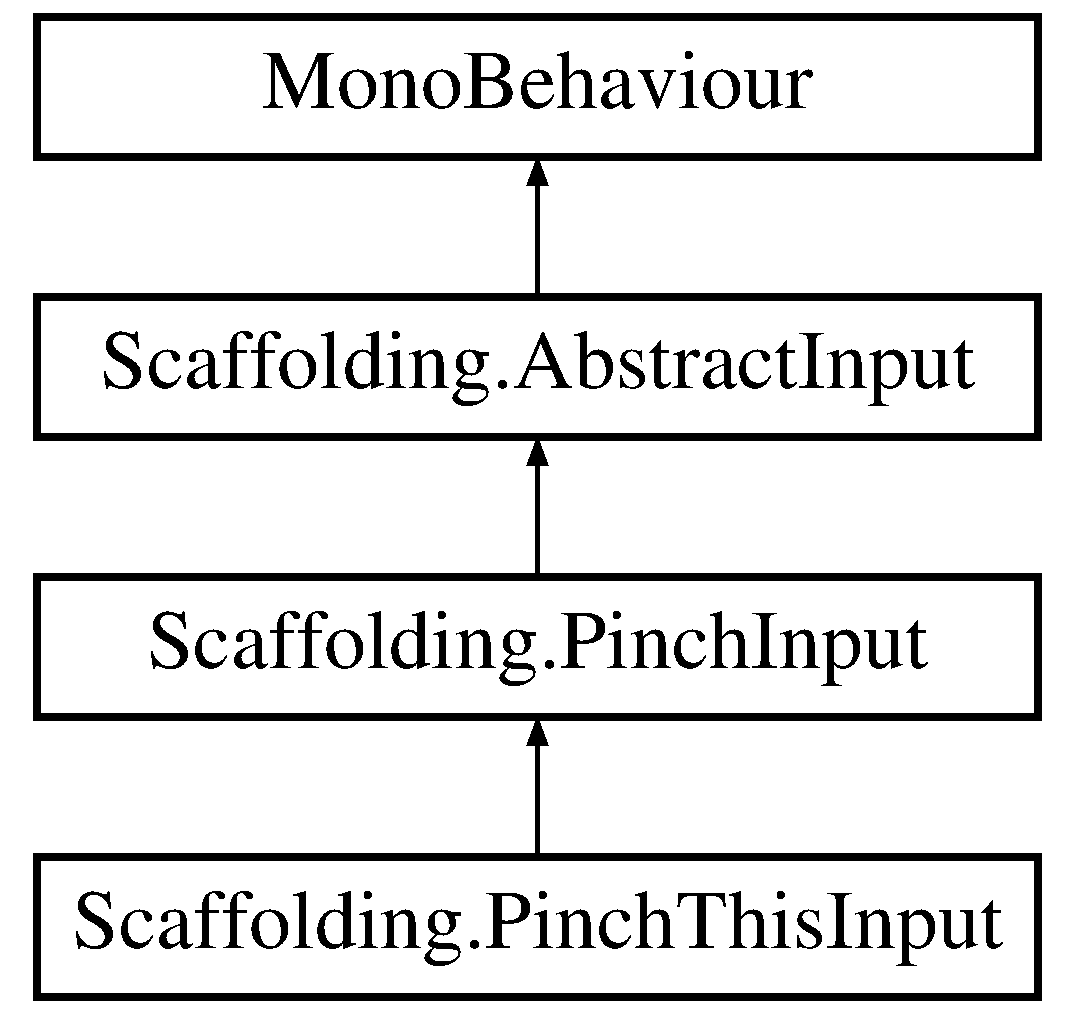
\includegraphics[height=4.000000cm]{class_scaffolding_1_1_pinch_this_input}
\end{center}
\end{figure}
\subsection*{Public Member Functions}
\begin{DoxyCompactItemize}
\item 
override void \hyperlink{class_scaffolding_1_1_pinch_this_input_a60b5bc5461de1286d8bd142742451dab}{Setup} (\hyperlink{class_scaffolding_1_1_abstract_view}{Abstract\+View} view)
\begin{DoxyCompactList}\small\item\em Run by the view during it's setup phase. \end{DoxyCompactList}\item 
override void \hyperlink{class_scaffolding_1_1_pinch_this_input_a00f941bc53b1847a2be7a2e61a4a9a57}{Handle\+Event\+Pressed} (\hyperlink{class_scaffolding_1_1_input_tracker}{Input\+Tracker} tracker)
\begin{DoxyCompactList}\small\item\em Event\+Pressed, dispatched by Scaffoldings \hyperlink{class_scaffolding_1_1_input_manager}{Input\+Manager} Passes through a \hyperlink{class_scaffolding_1_1_input_tracker}{Input\+Tracker} of the current touch. \end{DoxyCompactList}\item 
override void \hyperlink{class_scaffolding_1_1_pinch_this_input_ad9ca7c0e4b14d3d59ff06b258b4b9f7d}{Handle\+Event\+Released} (\hyperlink{class_scaffolding_1_1_input_tracker}{Input\+Tracker} tracker)
\begin{DoxyCompactList}\small\item\em Event\+Released, dispatched by Scaffoldings \hyperlink{class_scaffolding_1_1_input_manager}{Input\+Manager} Passes through a \hyperlink{class_scaffolding_1_1_input_tracker}{Input\+Tracker} of the current touch. \end{DoxyCompactList}\end{DoxyCompactItemize}
\subsection*{Public Attributes}
\begin{DoxyCompactItemize}
\item 
\hypertarget{class_scaffolding_1_1_pinch_this_input_ae6d32155af42acf9b1316c874626b2b4}{string {\bfseries input\+Camera}}\label{class_scaffolding_1_1_pinch_this_input_ae6d32155af42acf9b1316c874626b2b4}

\item 
\hypertarget{class_scaffolding_1_1_pinch_this_input_a52967dabb3c854e6aeb501f3423feb0d}{int {\bfseries input\+Camera\+Index}}\label{class_scaffolding_1_1_pinch_this_input_a52967dabb3c854e6aeb501f3423feb0d}

\item 
\hypertarget{class_scaffolding_1_1_pinch_this_input_a8c0727e05a84d7ee4e9136b728302f77}{int {\bfseries input\+Camera\+Length}}\label{class_scaffolding_1_1_pinch_this_input_a8c0727e05a84d7ee4e9136b728302f77}

\item 
\hypertarget{class_scaffolding_1_1_pinch_this_input_acb30c6b37a2031dccf9951608e247136}{float {\bfseries smallest\+Scale} = 0}\label{class_scaffolding_1_1_pinch_this_input_acb30c6b37a2031dccf9951608e247136}

\item 
\hypertarget{class_scaffolding_1_1_pinch_this_input_af682306ce14b0aea6fae51486784857e}{float {\bfseries largest\+Scale} = 2}\label{class_scaffolding_1_1_pinch_this_input_af682306ce14b0aea6fae51486784857e}

\end{DoxyCompactItemize}


\subsection{Detailed Description}
\hyperlink{class_scaffolding_1_1_pinch_this_input}{Pinch\+This\+Input} attaches to a gameobject as a quick solution to get something to respond to the pinch gesture. Extends \hyperlink{class_scaffolding_1_1_abstract_input}{Abstract\+Input} so falls under the same rules as other inputs in regards to views. E.\+g colliders get disabled during On\+Show\+Start and On\+Hide\+Start phases. 

Can be tested in the editor by holding down left C\+M\+D on mac or left C\+T\+R\+L on P\+C.\+Pinch this input. 

\subsection{Member Function Documentation}
\hypertarget{class_scaffolding_1_1_pinch_this_input_a00f941bc53b1847a2be7a2e61a4a9a57}{\index{Scaffolding\+::\+Pinch\+This\+Input@{Scaffolding\+::\+Pinch\+This\+Input}!Handle\+Event\+Pressed@{Handle\+Event\+Pressed}}
\index{Handle\+Event\+Pressed@{Handle\+Event\+Pressed}!Scaffolding\+::\+Pinch\+This\+Input@{Scaffolding\+::\+Pinch\+This\+Input}}
\subsubsection[{Handle\+Event\+Pressed}]{\setlength{\rightskip}{0pt plus 5cm}override void Scaffolding.\+Pinch\+This\+Input.\+Handle\+Event\+Pressed (
\begin{DoxyParamCaption}
\item[{{\bf Input\+Tracker}}]{tracker}
\end{DoxyParamCaption}
)\hspace{0.3cm}{\ttfamily [virtual]}}}\label{class_scaffolding_1_1_pinch_this_input_a00f941bc53b1847a2be7a2e61a4a9a57}


Event\+Pressed, dispatched by Scaffoldings \hyperlink{class_scaffolding_1_1_input_manager}{Input\+Manager} Passes through a \hyperlink{class_scaffolding_1_1_input_tracker}{Input\+Tracker} of the current touch. 


\begin{DoxyParams}{Parameters}
{\em tracker} & Tracker.\\
\hline
\end{DoxyParams}


Reimplemented from \hyperlink{class_scaffolding_1_1_pinch_input_aea53be8e94bef95c8373dd05639eaa41}{Scaffolding.\+Pinch\+Input}.

\hypertarget{class_scaffolding_1_1_pinch_this_input_ad9ca7c0e4b14d3d59ff06b258b4b9f7d}{\index{Scaffolding\+::\+Pinch\+This\+Input@{Scaffolding\+::\+Pinch\+This\+Input}!Handle\+Event\+Released@{Handle\+Event\+Released}}
\index{Handle\+Event\+Released@{Handle\+Event\+Released}!Scaffolding\+::\+Pinch\+This\+Input@{Scaffolding\+::\+Pinch\+This\+Input}}
\subsubsection[{Handle\+Event\+Released}]{\setlength{\rightskip}{0pt plus 5cm}override void Scaffolding.\+Pinch\+This\+Input.\+Handle\+Event\+Released (
\begin{DoxyParamCaption}
\item[{{\bf Input\+Tracker}}]{tracker}
\end{DoxyParamCaption}
)\hspace{0.3cm}{\ttfamily [virtual]}}}\label{class_scaffolding_1_1_pinch_this_input_ad9ca7c0e4b14d3d59ff06b258b4b9f7d}


Event\+Released, dispatched by Scaffoldings \hyperlink{class_scaffolding_1_1_input_manager}{Input\+Manager} Passes through a \hyperlink{class_scaffolding_1_1_input_tracker}{Input\+Tracker} of the current touch. 


\begin{DoxyParams}{Parameters}
{\em tracker} & Tracker.\\
\hline
\end{DoxyParams}


Reimplemented from \hyperlink{class_scaffolding_1_1_pinch_input_ad7e6fa3689011526acda972b7f6f4aa8}{Scaffolding.\+Pinch\+Input}.

\hypertarget{class_scaffolding_1_1_pinch_this_input_a60b5bc5461de1286d8bd142742451dab}{\index{Scaffolding\+::\+Pinch\+This\+Input@{Scaffolding\+::\+Pinch\+This\+Input}!Setup@{Setup}}
\index{Setup@{Setup}!Scaffolding\+::\+Pinch\+This\+Input@{Scaffolding\+::\+Pinch\+This\+Input}}
\subsubsection[{Setup}]{\setlength{\rightskip}{0pt plus 5cm}override void Scaffolding.\+Pinch\+This\+Input.\+Setup (
\begin{DoxyParamCaption}
\item[{{\bf Abstract\+View}}]{view}
\end{DoxyParamCaption}
)\hspace{0.3cm}{\ttfamily [virtual]}}}\label{class_scaffolding_1_1_pinch_this_input_a60b5bc5461de1286d8bd142742451dab}


Run by the view during it's setup phase. 


\begin{DoxyParams}{Parameters}
{\em view} & View.\\
\hline
\end{DoxyParams}


Reimplemented from \hyperlink{class_scaffolding_1_1_pinch_input_aa6687d25d10c2f4e7106641e0647af35}{Scaffolding.\+Pinch\+Input}.



The documentation for this class was generated from the following file\+:\begin{DoxyCompactItemize}
\item 
Input/\+Items/Pinch\+This\+Input.\+cs\end{DoxyCompactItemize}

\hypertarget{class_scaffolding_1_1_position_item}{\section{Scaffolding.\+Position\+Item Class Reference}
\label{class_scaffolding_1_1_position_item}\index{Scaffolding.\+Position\+Item@{Scaffolding.\+Position\+Item}}
}


Positions the transform relative to a camera. Only works with Orthographic cameras currently.  


Inheritance diagram for Scaffolding.\+Position\+Item\+:\begin{figure}[H]
\begin{center}
\leavevmode
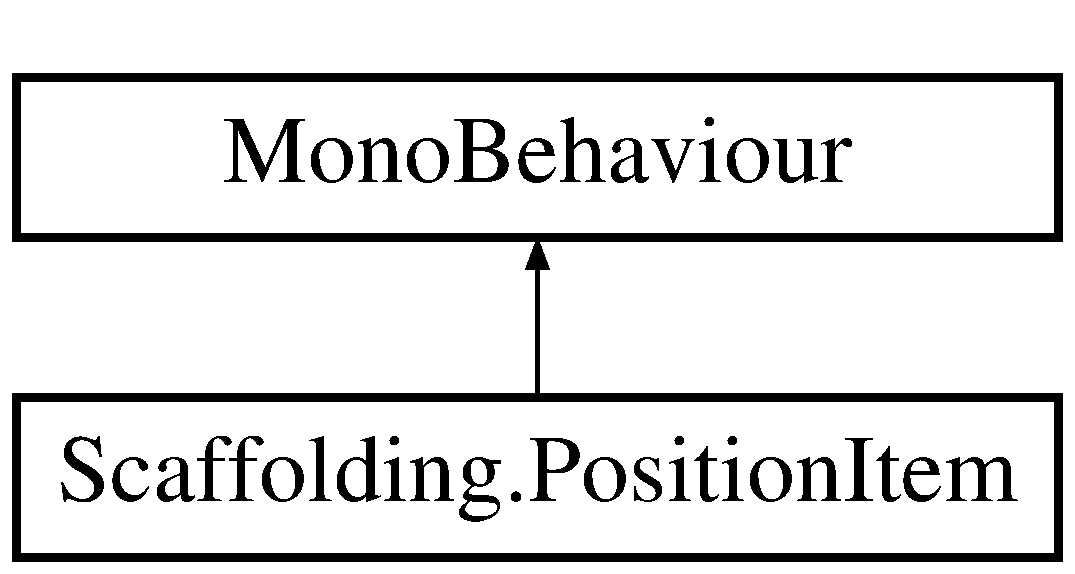
\includegraphics[height=2.000000cm]{class_scaffolding_1_1_position_item}
\end{center}
\end{figure}
\subsection*{Public Types}
\begin{DoxyCompactItemize}
\item 
\hypertarget{class_scaffolding_1_1_position_item_a4045eacf961abf4a013e76d3ac247e0b}{enum {\bfseries Screen\+Position} \{ \\*
{\bfseries None}, 
{\bfseries Upper\+Left}, 
{\bfseries Upper\+Middle}, 
{\bfseries Upper\+Right}, 
\\*
{\bfseries Left}, 
{\bfseries Middle}, 
{\bfseries Right}, 
{\bfseries Lower\+Left}, 
\\*
{\bfseries Lower\+Middle}, 
{\bfseries Lower\+Right}
 \}}\label{class_scaffolding_1_1_position_item_a4045eacf961abf4a013e76d3ac247e0b}

\end{DoxyCompactItemize}
\subsection*{Public Member Functions}
\begin{DoxyCompactItemize}
\item 
void \hyperlink{class_scaffolding_1_1_position_item_acf8866c7ad64b0d81429c5dfa95482fd}{Set\+Position} ()
\begin{DoxyCompactList}\small\item\em Resets the position to its current configuration. Used when the screen size has changed. \end{DoxyCompactList}\end{DoxyCompactItemize}
\subsection*{Public Attributes}
\begin{DoxyCompactItemize}
\item 
\hypertarget{class_scaffolding_1_1_position_item_ae379bb2d0a5411db8b5d5fd8e54009a9}{Screen\+Position {\bfseries screen\+Position}}\label{class_scaffolding_1_1_position_item_ae379bb2d0a5411db8b5d5fd8e54009a9}

\item 
\hypertarget{class_scaffolding_1_1_position_item_a35c7b90de17784ca76a00de4527e4ac0}{Vector2 {\bfseries edge\+Buffer}}\label{class_scaffolding_1_1_position_item_a35c7b90de17784ca76a00de4527e4ac0}

\item 
\hypertarget{class_scaffolding_1_1_position_item_abb57beebd4d760f158c41eab1605b03b}{string {\bfseries rendering\+Camera}}\label{class_scaffolding_1_1_position_item_abb57beebd4d760f158c41eab1605b03b}

\item 
\hypertarget{class_scaffolding_1_1_position_item_acd670d2adf3d2d9c283d1fcee184b83f}{int {\bfseries rendering\+Camera\+Index}}\label{class_scaffolding_1_1_position_item_acd670d2adf3d2d9c283d1fcee184b83f}

\item 
\hypertarget{class_scaffolding_1_1_position_item_aa262b417dd78ff97214c9e39669a0bc3}{int {\bfseries rendering\+Camera\+Length}}\label{class_scaffolding_1_1_position_item_aa262b417dd78ff97214c9e39669a0bc3}

\end{DoxyCompactItemize}


\subsection{Detailed Description}
Positions the transform relative to a camera. Only works with Orthographic cameras currently. 



\subsection{Member Function Documentation}
\hypertarget{class_scaffolding_1_1_position_item_acf8866c7ad64b0d81429c5dfa95482fd}{\index{Scaffolding\+::\+Position\+Item@{Scaffolding\+::\+Position\+Item}!Set\+Position@{Set\+Position}}
\index{Set\+Position@{Set\+Position}!Scaffolding\+::\+Position\+Item@{Scaffolding\+::\+Position\+Item}}
\subsubsection[{Set\+Position}]{\setlength{\rightskip}{0pt plus 5cm}void Scaffolding.\+Position\+Item.\+Set\+Position (
\begin{DoxyParamCaption}
{}
\end{DoxyParamCaption}
)}}\label{class_scaffolding_1_1_position_item_acf8866c7ad64b0d81429c5dfa95482fd}


Resets the position to its current configuration. Used when the screen size has changed. 



The documentation for this class was generated from the following file\+:\begin{DoxyCompactItemize}
\item 
Input/\+Items/Position\+Item.\+cs\end{DoxyCompactItemize}

\hypertarget{class_scaffolding_1_1_rotate_input}{\section{Scaffolding.\-Rotate\-Input Class Reference}
\label{class_scaffolding_1_1_rotate_input}\index{Scaffolding.\-Rotate\-Input@{Scaffolding.\-Rotate\-Input}}
}


Rotate input is largely a touch input based class. It replicates the rotate gesture, and dispatches a callback while rotating.  


Inheritance diagram for Scaffolding.\-Rotate\-Input\-:\begin{figure}[H]
\begin{center}
\leavevmode
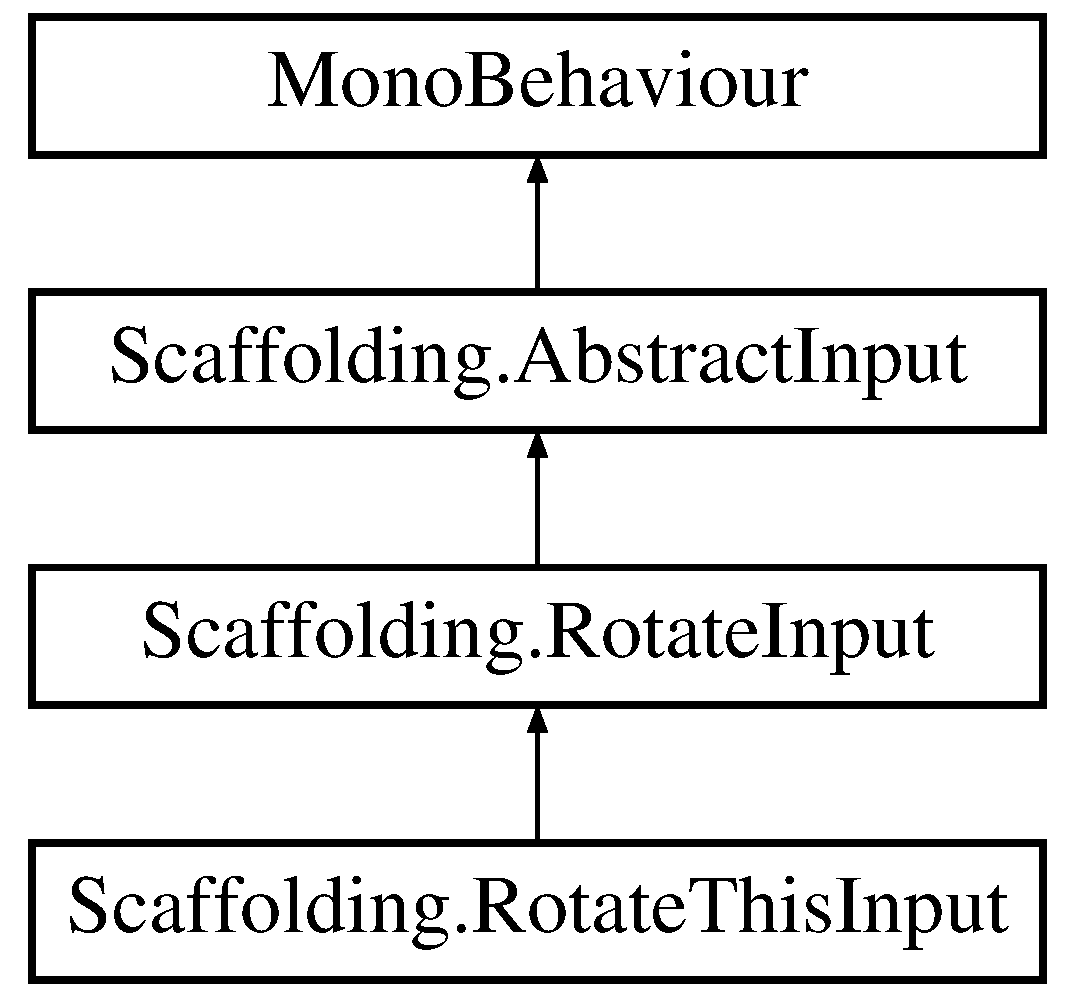
\includegraphics[height=4.000000cm]{class_scaffolding_1_1_rotate_input}
\end{center}
\end{figure}
\subsection*{Public Member Functions}
\begin{DoxyCompactItemize}
\item 
override void \hyperlink{class_scaffolding_1_1_rotate_input_a89be6ed5c624ff8f637fdc38227c4637}{Setup} (\hyperlink{class_scaffolding_1_1_abstract_view}{Abstract\-View} view)
\begin{DoxyCompactList}\small\item\em Run by the view during it's setup phase. \end{DoxyCompactList}\item 
override void \hyperlink{class_scaffolding_1_1_rotate_input_a85778a91b86665998c1b84f24c571e88}{Cleanup} ()
\begin{DoxyCompactList}\small\item\em The inputs clean up phase. \end{DoxyCompactList}\item 
void \hyperlink{class_scaffolding_1_1_rotate_input_a07b51f4f3db3e4e041f45a011319f8d9}{Register\-Rotate\-Callback} (Action$<$ float $>$ callback)
\begin{DoxyCompactList}\small\item\em Register a callback handler for rotation. \end{DoxyCompactList}\item 
override void \hyperlink{class_scaffolding_1_1_rotate_input_a4c37089dcaae6d1cb1785b45d5cec8b3}{Handle\-Event\-Pressed} (\hyperlink{class_scaffolding_1_1_input_tracker}{Input\-Tracker} tracker)
\begin{DoxyCompactList}\small\item\em Event\-Pressed, dispatched by Scaffoldings \hyperlink{class_scaffolding_1_1_input_manager}{Input\-Manager} Passes through a \hyperlink{class_scaffolding_1_1_input_tracker}{Input\-Tracker} of the current touch. \end{DoxyCompactList}\item 
override void \hyperlink{class_scaffolding_1_1_rotate_input_afffb85f2f27b314bde50d0e45d6117d5}{Handle\-Event\-Dragged} (\hyperlink{class_scaffolding_1_1_input_tracker}{Input\-Tracker} tracker)
\begin{DoxyCompactList}\small\item\em Event\-Dragged, dispatched by Scaffoldings \hyperlink{class_scaffolding_1_1_input_manager}{Input\-Manager} Passes through a \hyperlink{class_scaffolding_1_1_input_tracker}{Input\-Tracker} of the current touch. \end{DoxyCompactList}\item 
override void \hyperlink{class_scaffolding_1_1_rotate_input_a96588e29dafafeb2e1e1c5469b2bbda1}{Handle\-Event\-Released} (\hyperlink{class_scaffolding_1_1_input_tracker}{Input\-Tracker} tracker)
\begin{DoxyCompactList}\small\item\em Event\-Released, dispatched by Scaffoldings \hyperlink{class_scaffolding_1_1_input_manager}{Input\-Manager} Passes through a \hyperlink{class_scaffolding_1_1_input_tracker}{Input\-Tracker} of the current touch. \end{DoxyCompactList}\end{DoxyCompactItemize}


\subsection{Detailed Description}
Rotate input is largely a touch input based class. It replicates the rotate gesture, and dispatches a callback while rotating. 



\subsection{Member Function Documentation}
\hypertarget{class_scaffolding_1_1_rotate_input_a85778a91b86665998c1b84f24c571e88}{\index{Scaffolding\-::\-Rotate\-Input@{Scaffolding\-::\-Rotate\-Input}!Cleanup@{Cleanup}}
\index{Cleanup@{Cleanup}!Scaffolding::RotateInput@{Scaffolding\-::\-Rotate\-Input}}
\subsubsection[{Cleanup}]{\setlength{\rightskip}{0pt plus 5cm}override void Scaffolding.\-Rotate\-Input.\-Cleanup (
\begin{DoxyParamCaption}
{}
\end{DoxyParamCaption}
)\hspace{0.3cm}{\ttfamily [virtual]}}}\label{class_scaffolding_1_1_rotate_input_a85778a91b86665998c1b84f24c571e88}


The inputs clean up phase. 



Reimplemented from \hyperlink{class_scaffolding_1_1_abstract_input_ab179ae99e76c6c934a0dcba4fc195e68}{Scaffolding.\-Abstract\-Input}.

\hypertarget{class_scaffolding_1_1_rotate_input_afffb85f2f27b314bde50d0e45d6117d5}{\index{Scaffolding\-::\-Rotate\-Input@{Scaffolding\-::\-Rotate\-Input}!Handle\-Event\-Dragged@{Handle\-Event\-Dragged}}
\index{Handle\-Event\-Dragged@{Handle\-Event\-Dragged}!Scaffolding::RotateInput@{Scaffolding\-::\-Rotate\-Input}}
\subsubsection[{Handle\-Event\-Dragged}]{\setlength{\rightskip}{0pt plus 5cm}override void Scaffolding.\-Rotate\-Input.\-Handle\-Event\-Dragged (
\begin{DoxyParamCaption}
\item[{{\bf Input\-Tracker}}]{tracker}
\end{DoxyParamCaption}
)\hspace{0.3cm}{\ttfamily [virtual]}}}\label{class_scaffolding_1_1_rotate_input_afffb85f2f27b314bde50d0e45d6117d5}


Event\-Dragged, dispatched by Scaffoldings \hyperlink{class_scaffolding_1_1_input_manager}{Input\-Manager} Passes through a \hyperlink{class_scaffolding_1_1_input_tracker}{Input\-Tracker} of the current touch. 


\begin{DoxyParams}{Parameters}
{\em tracker} & Tracker.\\
\hline
\end{DoxyParams}


Reimplemented from \hyperlink{class_scaffolding_1_1_abstract_input_a5996b0cb611a384e527ce871b9607858}{Scaffolding.\-Abstract\-Input}.

\hypertarget{class_scaffolding_1_1_rotate_input_a4c37089dcaae6d1cb1785b45d5cec8b3}{\index{Scaffolding\-::\-Rotate\-Input@{Scaffolding\-::\-Rotate\-Input}!Handle\-Event\-Pressed@{Handle\-Event\-Pressed}}
\index{Handle\-Event\-Pressed@{Handle\-Event\-Pressed}!Scaffolding::RotateInput@{Scaffolding\-::\-Rotate\-Input}}
\subsubsection[{Handle\-Event\-Pressed}]{\setlength{\rightskip}{0pt plus 5cm}override void Scaffolding.\-Rotate\-Input.\-Handle\-Event\-Pressed (
\begin{DoxyParamCaption}
\item[{{\bf Input\-Tracker}}]{tracker}
\end{DoxyParamCaption}
)\hspace{0.3cm}{\ttfamily [virtual]}}}\label{class_scaffolding_1_1_rotate_input_a4c37089dcaae6d1cb1785b45d5cec8b3}


Event\-Pressed, dispatched by Scaffoldings \hyperlink{class_scaffolding_1_1_input_manager}{Input\-Manager} Passes through a \hyperlink{class_scaffolding_1_1_input_tracker}{Input\-Tracker} of the current touch. 


\begin{DoxyParams}{Parameters}
{\em tracker} & Tracker.\\
\hline
\end{DoxyParams}


Reimplemented from \hyperlink{class_scaffolding_1_1_abstract_input_a11e83c3462719749f8281a21024e902f}{Scaffolding.\-Abstract\-Input}.



Reimplemented in \hyperlink{class_scaffolding_1_1_rotate_this_input_a721eb598cb78a1abb06d8c37f9de01ea}{Scaffolding.\-Rotate\-This\-Input}.

\hypertarget{class_scaffolding_1_1_rotate_input_a96588e29dafafeb2e1e1c5469b2bbda1}{\index{Scaffolding\-::\-Rotate\-Input@{Scaffolding\-::\-Rotate\-Input}!Handle\-Event\-Released@{Handle\-Event\-Released}}
\index{Handle\-Event\-Released@{Handle\-Event\-Released}!Scaffolding::RotateInput@{Scaffolding\-::\-Rotate\-Input}}
\subsubsection[{Handle\-Event\-Released}]{\setlength{\rightskip}{0pt plus 5cm}override void Scaffolding.\-Rotate\-Input.\-Handle\-Event\-Released (
\begin{DoxyParamCaption}
\item[{{\bf Input\-Tracker}}]{tracker}
\end{DoxyParamCaption}
)\hspace{0.3cm}{\ttfamily [virtual]}}}\label{class_scaffolding_1_1_rotate_input_a96588e29dafafeb2e1e1c5469b2bbda1}


Event\-Released, dispatched by Scaffoldings \hyperlink{class_scaffolding_1_1_input_manager}{Input\-Manager} Passes through a \hyperlink{class_scaffolding_1_1_input_tracker}{Input\-Tracker} of the current touch. 


\begin{DoxyParams}{Parameters}
{\em tracker} & Tracker.\\
\hline
\end{DoxyParams}


Reimplemented from \hyperlink{class_scaffolding_1_1_abstract_input_a11854454457cd55a26f345011f4bd6bc}{Scaffolding.\-Abstract\-Input}.



Reimplemented in \hyperlink{class_scaffolding_1_1_rotate_this_input_aa90af18d3d575cb5a5176e3c952e68cd}{Scaffolding.\-Rotate\-This\-Input}.

\hypertarget{class_scaffolding_1_1_rotate_input_a07b51f4f3db3e4e041f45a011319f8d9}{\index{Scaffolding\-::\-Rotate\-Input@{Scaffolding\-::\-Rotate\-Input}!Register\-Rotate\-Callback@{Register\-Rotate\-Callback}}
\index{Register\-Rotate\-Callback@{Register\-Rotate\-Callback}!Scaffolding::RotateInput@{Scaffolding\-::\-Rotate\-Input}}
\subsubsection[{Register\-Rotate\-Callback}]{\setlength{\rightskip}{0pt plus 5cm}void Scaffolding.\-Rotate\-Input.\-Register\-Rotate\-Callback (
\begin{DoxyParamCaption}
\item[{Action$<$ float $>$}]{callback}
\end{DoxyParamCaption}
)}}\label{class_scaffolding_1_1_rotate_input_a07b51f4f3db3e4e041f45a011319f8d9}


Register a callback handler for rotation. 

Example\-: public void My\-Callback\-Function(float delta\-Angle) \{ //do rotation based code here... \}

\-\_\-rotate\-Input.\-Register\-Rotate\-Callback(\-My\-Callback\-Function);


\begin{DoxyParams}{Parameters}
{\em callback} & Callback.\\
\hline
\end{DoxyParams}
\hypertarget{class_scaffolding_1_1_rotate_input_a89be6ed5c624ff8f637fdc38227c4637}{\index{Scaffolding\-::\-Rotate\-Input@{Scaffolding\-::\-Rotate\-Input}!Setup@{Setup}}
\index{Setup@{Setup}!Scaffolding::RotateInput@{Scaffolding\-::\-Rotate\-Input}}
\subsubsection[{Setup}]{\setlength{\rightskip}{0pt plus 5cm}override void Scaffolding.\-Rotate\-Input.\-Setup (
\begin{DoxyParamCaption}
\item[{{\bf Abstract\-View}}]{view}
\end{DoxyParamCaption}
)\hspace{0.3cm}{\ttfamily [virtual]}}}\label{class_scaffolding_1_1_rotate_input_a89be6ed5c624ff8f637fdc38227c4637}


Run by the view during it's setup phase. 


\begin{DoxyParams}{Parameters}
{\em view} & View.\\
\hline
\end{DoxyParams}


Reimplemented from \hyperlink{class_scaffolding_1_1_abstract_input_a598859c6342920d2b0c985310e6e9476}{Scaffolding.\-Abstract\-Input}.



Reimplemented in \hyperlink{class_scaffolding_1_1_rotate_this_input_a9e0fc73644310f1efd1f49e692638c89}{Scaffolding.\-Rotate\-This\-Input}.



The documentation for this class was generated from the following file\-:\begin{DoxyCompactItemize}
\item 
Input/\-Items/Rotate\-Input.\-cs\end{DoxyCompactItemize}

\hypertarget{class_scaffolding_1_1_rotate_this_input}{\section{Scaffolding.\+Rotate\+This\+Input Class Reference}
\label{class_scaffolding_1_1_rotate_this_input}\index{Scaffolding.\+Rotate\+This\+Input@{Scaffolding.\+Rotate\+This\+Input}}
}


\hyperlink{class_scaffolding_1_1_rotate_this_input}{Rotate\+This\+Input} attaches to a gameobject as a quick solution to get something to respond to the rotate gesture. Extends \hyperlink{class_scaffolding_1_1_abstract_input}{Abstract\+Input} so falls under the same rules as other inputs in regards to views. E.\+g colliders get disabled during On\+Show\+Start and On\+Hide\+Start phases.  


Inheritance diagram for Scaffolding.\+Rotate\+This\+Input\+:\begin{figure}[H]
\begin{center}
\leavevmode
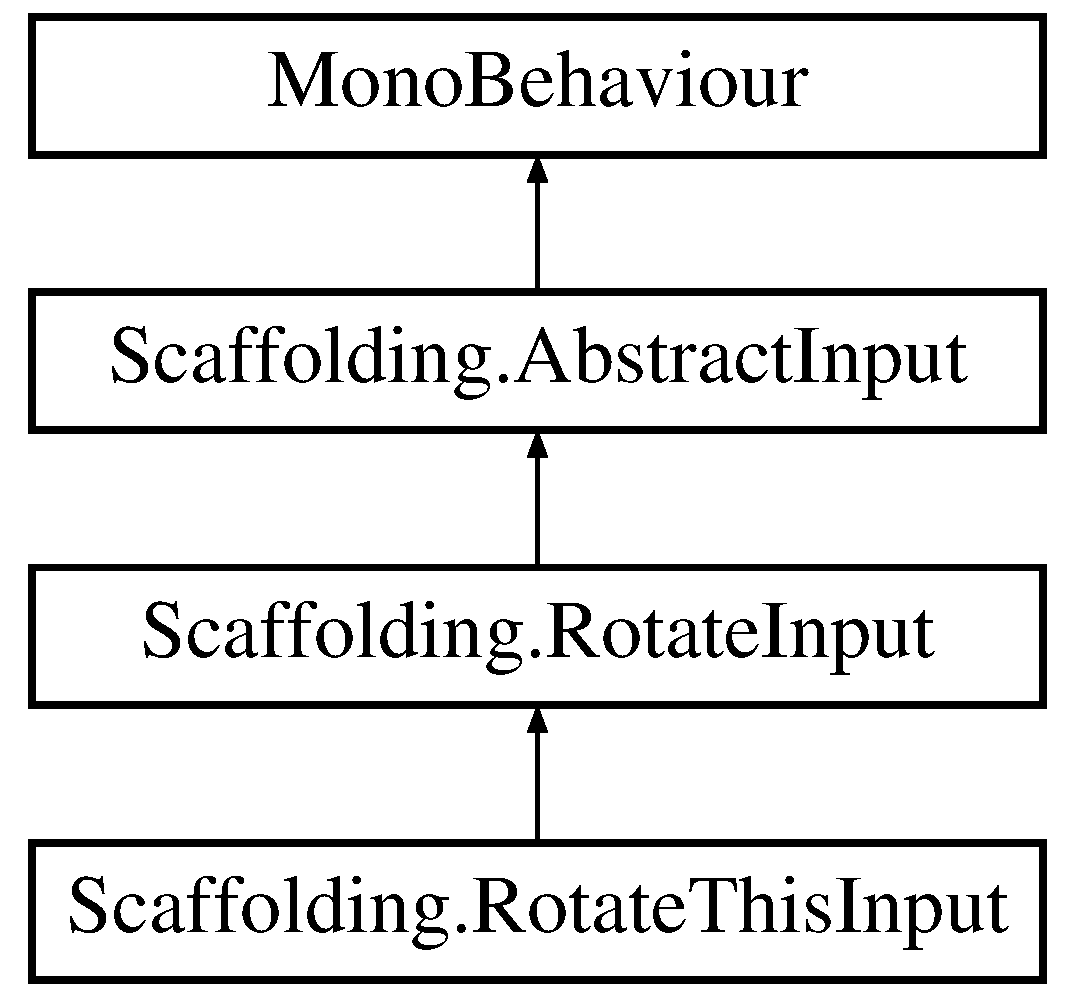
\includegraphics[height=4.000000cm]{class_scaffolding_1_1_rotate_this_input}
\end{center}
\end{figure}
\subsection*{Public Member Functions}
\begin{DoxyCompactItemize}
\item 
override void \hyperlink{class_scaffolding_1_1_rotate_this_input_a9e0fc73644310f1efd1f49e692638c89}{Setup} (\hyperlink{class_scaffolding_1_1_abstract_view}{Abstract\+View} view)
\begin{DoxyCompactList}\small\item\em Run by the view during it's setup phase. \end{DoxyCompactList}\item 
override void \hyperlink{class_scaffolding_1_1_rotate_this_input_a721eb598cb78a1abb06d8c37f9de01ea}{Handle\+Event\+Pressed} (\hyperlink{class_scaffolding_1_1_input_tracker}{Input\+Tracker} tracker)
\begin{DoxyCompactList}\small\item\em Event\+Pressed, dispatched by Scaffoldings \hyperlink{class_scaffolding_1_1_input_manager}{Input\+Manager} Passes through a \hyperlink{class_scaffolding_1_1_input_tracker}{Input\+Tracker} of the current touch. \end{DoxyCompactList}\item 
override void \hyperlink{class_scaffolding_1_1_rotate_this_input_aa90af18d3d575cb5a5176e3c952e68cd}{Handle\+Event\+Released} (\hyperlink{class_scaffolding_1_1_input_tracker}{Input\+Tracker} tracker)
\begin{DoxyCompactList}\small\item\em Event\+Released, dispatched by Scaffoldings \hyperlink{class_scaffolding_1_1_input_manager}{Input\+Manager} Passes through a \hyperlink{class_scaffolding_1_1_input_tracker}{Input\+Tracker} of the current touch. \end{DoxyCompactList}\end{DoxyCompactItemize}
\subsection*{Public Attributes}
\begin{DoxyCompactItemize}
\item 
\hypertarget{class_scaffolding_1_1_rotate_this_input_a2d2bf1c1f8339c1f2dba78c68888ba40}{string {\bfseries input\+Camera}}\label{class_scaffolding_1_1_rotate_this_input_a2d2bf1c1f8339c1f2dba78c68888ba40}

\item 
\hypertarget{class_scaffolding_1_1_rotate_this_input_afb50ecc538a545891be6647d1f615961}{int {\bfseries input\+Camera\+Index}}\label{class_scaffolding_1_1_rotate_this_input_afb50ecc538a545891be6647d1f615961}

\item 
\hypertarget{class_scaffolding_1_1_rotate_this_input_af55328f2f51d26f738238dec61eb308b}{int {\bfseries input\+Camera\+Length}}\label{class_scaffolding_1_1_rotate_this_input_af55328f2f51d26f738238dec61eb308b}

\end{DoxyCompactItemize}


\subsection{Detailed Description}
\hyperlink{class_scaffolding_1_1_rotate_this_input}{Rotate\+This\+Input} attaches to a gameobject as a quick solution to get something to respond to the rotate gesture. Extends \hyperlink{class_scaffolding_1_1_abstract_input}{Abstract\+Input} so falls under the same rules as other inputs in regards to views. E.\+g colliders get disabled during On\+Show\+Start and On\+Hide\+Start phases. 

Can be tested in the editor by holding down left C\+M\+D on mac or left C\+T\+R\+L on P\+C. 

\subsection{Member Function Documentation}
\hypertarget{class_scaffolding_1_1_rotate_this_input_a721eb598cb78a1abb06d8c37f9de01ea}{\index{Scaffolding\+::\+Rotate\+This\+Input@{Scaffolding\+::\+Rotate\+This\+Input}!Handle\+Event\+Pressed@{Handle\+Event\+Pressed}}
\index{Handle\+Event\+Pressed@{Handle\+Event\+Pressed}!Scaffolding\+::\+Rotate\+This\+Input@{Scaffolding\+::\+Rotate\+This\+Input}}
\subsubsection[{Handle\+Event\+Pressed}]{\setlength{\rightskip}{0pt plus 5cm}override void Scaffolding.\+Rotate\+This\+Input.\+Handle\+Event\+Pressed (
\begin{DoxyParamCaption}
\item[{{\bf Input\+Tracker}}]{tracker}
\end{DoxyParamCaption}
)\hspace{0.3cm}{\ttfamily [virtual]}}}\label{class_scaffolding_1_1_rotate_this_input_a721eb598cb78a1abb06d8c37f9de01ea}


Event\+Pressed, dispatched by Scaffoldings \hyperlink{class_scaffolding_1_1_input_manager}{Input\+Manager} Passes through a \hyperlink{class_scaffolding_1_1_input_tracker}{Input\+Tracker} of the current touch. 


\begin{DoxyParams}{Parameters}
{\em tracker} & Tracker.\\
\hline
\end{DoxyParams}


Reimplemented from \hyperlink{class_scaffolding_1_1_rotate_input_a4c37089dcaae6d1cb1785b45d5cec8b3}{Scaffolding.\+Rotate\+Input}.

\hypertarget{class_scaffolding_1_1_rotate_this_input_aa90af18d3d575cb5a5176e3c952e68cd}{\index{Scaffolding\+::\+Rotate\+This\+Input@{Scaffolding\+::\+Rotate\+This\+Input}!Handle\+Event\+Released@{Handle\+Event\+Released}}
\index{Handle\+Event\+Released@{Handle\+Event\+Released}!Scaffolding\+::\+Rotate\+This\+Input@{Scaffolding\+::\+Rotate\+This\+Input}}
\subsubsection[{Handle\+Event\+Released}]{\setlength{\rightskip}{0pt plus 5cm}override void Scaffolding.\+Rotate\+This\+Input.\+Handle\+Event\+Released (
\begin{DoxyParamCaption}
\item[{{\bf Input\+Tracker}}]{tracker}
\end{DoxyParamCaption}
)\hspace{0.3cm}{\ttfamily [virtual]}}}\label{class_scaffolding_1_1_rotate_this_input_aa90af18d3d575cb5a5176e3c952e68cd}


Event\+Released, dispatched by Scaffoldings \hyperlink{class_scaffolding_1_1_input_manager}{Input\+Manager} Passes through a \hyperlink{class_scaffolding_1_1_input_tracker}{Input\+Tracker} of the current touch. 


\begin{DoxyParams}{Parameters}
{\em tracker} & Tracker.\\
\hline
\end{DoxyParams}


Reimplemented from \hyperlink{class_scaffolding_1_1_rotate_input_a96588e29dafafeb2e1e1c5469b2bbda1}{Scaffolding.\+Rotate\+Input}.

\hypertarget{class_scaffolding_1_1_rotate_this_input_a9e0fc73644310f1efd1f49e692638c89}{\index{Scaffolding\+::\+Rotate\+This\+Input@{Scaffolding\+::\+Rotate\+This\+Input}!Setup@{Setup}}
\index{Setup@{Setup}!Scaffolding\+::\+Rotate\+This\+Input@{Scaffolding\+::\+Rotate\+This\+Input}}
\subsubsection[{Setup}]{\setlength{\rightskip}{0pt plus 5cm}override void Scaffolding.\+Rotate\+This\+Input.\+Setup (
\begin{DoxyParamCaption}
\item[{{\bf Abstract\+View}}]{view}
\end{DoxyParamCaption}
)\hspace{0.3cm}{\ttfamily [virtual]}}}\label{class_scaffolding_1_1_rotate_this_input_a9e0fc73644310f1efd1f49e692638c89}


Run by the view during it's setup phase. 


\begin{DoxyParams}{Parameters}
{\em view} & View.\\
\hline
\end{DoxyParams}


Reimplemented from \hyperlink{class_scaffolding_1_1_rotate_input_a89be6ed5c624ff8f637fdc38227c4637}{Scaffolding.\+Rotate\+Input}.



The documentation for this class was generated from the following file\+:\begin{DoxyCompactItemize}
\item 
Input/\+Items/Rotate\+This\+Input.\+cs\end{DoxyCompactItemize}

\hypertarget{class_scaffolding_1_1_scaffolding_button}{\section{Scaffolding.\-Scaffolding\-Button Class Reference}
\label{class_scaffolding_1_1_scaffolding_button}\index{Scaffolding.\-Scaffolding\-Button@{Scaffolding.\-Scaffolding\-Button}}
}


The button class associated with the \hyperlink{namespace_scaffolding}{Scaffolding} default buttons.  


Inheritance diagram for Scaffolding.\-Scaffolding\-Button\-:\begin{figure}[H]
\begin{center}
\leavevmode
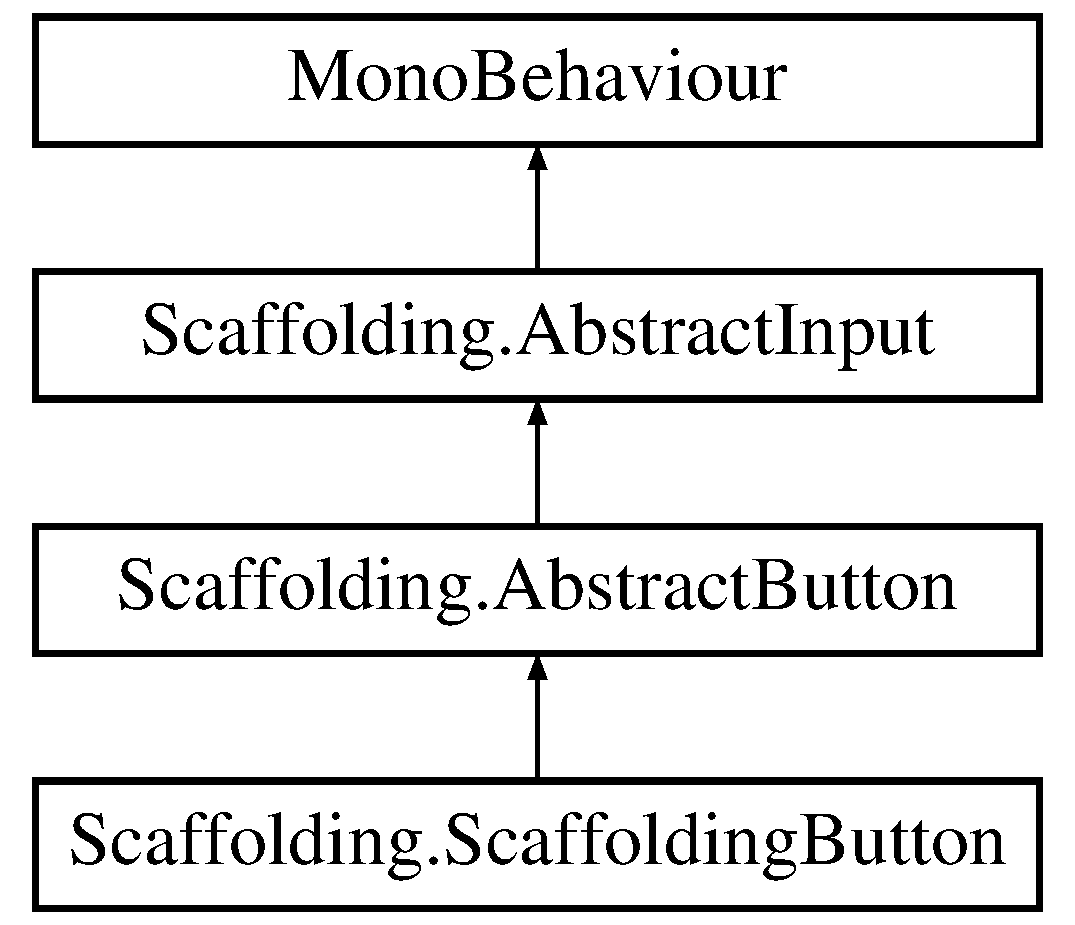
\includegraphics[height=3.000000cm]{class_scaffolding_1_1_scaffolding_button}
\end{center}
\end{figure}
\subsection*{Public Types}
\begin{DoxyCompactItemize}
\item 
enum {\bfseries Button\-Action\-Type} \{ {\bfseries Do\-Nothing}, 
{\bfseries Open}, 
{\bfseries Close}, 
{\bfseries Play\-An\-Animation}
 \}
\item 
enum {\bfseries Button\-State} \{ {\bfseries Up}, 
{\bfseries Down}, 
{\bfseries Inactive}
 \}
\end{DoxyCompactItemize}
\subsection*{Public Member Functions}
\begin{DoxyCompactItemize}
\item 
override void \hyperlink{class_scaffolding_1_1_scaffolding_button_a9473252a76f28a9d9605c7be23377f94}{Setup} (\hyperlink{class_scaffolding_1_1_abstract_view}{Abstract\-View} view)
\begin{DoxyCompactList}\small\item\em Run by the view during it's setup phase. \end{DoxyCompactList}\item 
override void \hyperlink{class_scaffolding_1_1_scaffolding_button_a1f295926babd2653cd63ed2933108d45}{Cleanup} ()
\begin{DoxyCompactList}\small\item\em Runs when parent view is closed, override this to clean up your extended button. \end{DoxyCompactList}\item 
override void \hyperlink{class_scaffolding_1_1_scaffolding_button_a1cc1e5b6b74c5411e1ca46dd81eb5144}{Handle\-Event\-Pressed} (\hyperlink{class_scaffolding_1_1_input_tracker}{Input\-Tracker} tracker)
\begin{DoxyCompactList}\small\item\em Event\-Pressed, dispatched by Scaffoldings \hyperlink{class_scaffolding_1_1_input_manager}{Input\-Manager} Passes through a \hyperlink{class_scaffolding_1_1_input_tracker}{Input\-Tracker} of the current touch. \end{DoxyCompactList}\item 
override void \hyperlink{class_scaffolding_1_1_scaffolding_button_ab6c3c337fc6c6c9dad69498ac5acd098}{Handle\-Event\-Released} (\hyperlink{class_scaffolding_1_1_input_tracker}{Input\-Tracker} tracker)
\begin{DoxyCompactList}\small\item\em Event\-Released, dispatched by Scaffoldings \hyperlink{class_scaffolding_1_1_input_manager}{Input\-Manager} Passes through a \hyperlink{class_scaffolding_1_1_input_tracker}{Input\-Tracker} of the current touch. \end{DoxyCompactList}\item 
override void \hyperlink{class_scaffolding_1_1_scaffolding_button_aa84a30d26afd5a3f54b5614d6e09e535}{Toggle\-Enabled\-Input} (bool enabled)
\begin{DoxyCompactList}\small\item\em Runs when view is closed or opened. Enables or Disables the button, and changes its visual state. \end{DoxyCompactList}\item 
void \hyperlink{class_scaffolding_1_1_scaffolding_button_aae1c0c4bf8e05652482aa08e5074a146}{Toggle\-Button\-Inactive} (bool active)
\begin{DoxyCompactList}\small\item\em Toggles the button inactive state. \end{DoxyCompactList}\item 
void \hyperlink{class_scaffolding_1_1_scaffolding_button_a46d64b651a64a4bffbe23ccba30eb62b}{Disable\-Inputs\-On\-Overlay} (Type t)
\begin{DoxyCompactList}\small\item\em Disables the inputs for an overlay. Use this when opening an overlay and you dont want any click throughs happening on the current view. \end{DoxyCompactList}\item 
void \hyperlink{class_scaffolding_1_1_scaffolding_button_a58b903748ef8c771beaf4ef2549d6e3a}{Open\-Screen\-On\-Pressed} (Type target\-View)
\begin{DoxyCompactList}\small\item\em Set the Screen to be opened when the button is pressed. \end{DoxyCompactList}\item 
void \hyperlink{class_scaffolding_1_1_scaffolding_button_acf69a55f5537c91b3ddb251054c5b00e}{Open\-Screen\-On\-Pressed} (Type target\-View, Type loading\-View)
\begin{DoxyCompactList}\small\item\em Set the screen to be opened when the button is pressed. Set the loading overlay to be opened first to mask heavy loading. \end{DoxyCompactList}\item 
void \hyperlink{class_scaffolding_1_1_scaffolding_button_a6a88c00f8269467d03e6809fa10735bd}{Open\-Overlay\-On\-Pressed} (Type target\-Overlay)
\begin{DoxyCompactList}\small\item\em Set the overlay to be opened when the button is pressed. \end{DoxyCompactList}\item 
void \hyperlink{class_scaffolding_1_1_scaffolding_button_ad0f4de72aa3f1d16675ab391a5cc7fac}{Close\-Overlay\-On\-Pressed} (Type target\-Overlay)
\begin{DoxyCompactList}\small\item\em Set the overlay to be closed when the button is pressed. \end{DoxyCompactList}\item 
void \hyperlink{class_scaffolding_1_1_scaffolding_button_a64d38c68237749eb7257c6bb29157af8}{Run\-Method\-On\-Pressed} (Type target\-Class, string method)
\begin{DoxyCompactList}\small\item\em Add a method to be called when the button is pressed. \end{DoxyCompactList}\item 
void \hyperlink{class_scaffolding_1_1_scaffolding_button_a14a7663cdb2337745c9da6eb49c27c84}{Add\-Button\-Pressed\-Handler} (Action$<$ \hyperlink{class_scaffolding_1_1_scaffolding_button}{Scaffolding\-Button} $>$ action)
\begin{DoxyCompactList}\small\item\em Registers the button pressed callback. \end{DoxyCompactList}\item 
void \hyperlink{class_scaffolding_1_1_scaffolding_button_a5857275c09f0c219bb7f5a5f2a345311}{Add\-Button\-Down\-Handler} (Action$<$ \hyperlink{class_scaffolding_1_1_scaffolding_button}{Scaffolding\-Button} $>$ action)
\begin{DoxyCompactList}\small\item\em Registers the button down callback. \end{DoxyCompactList}\end{DoxyCompactItemize}
\subsection*{Public Attributes}
\begin{DoxyCompactItemize}
\item 
\hypertarget{class_scaffolding_1_1_scaffolding_button_a20f7172d6e146170a2501484c2e84027}{string {\bfseries target\-View}}\label{class_scaffolding_1_1_scaffolding_button_a20f7172d6e146170a2501484c2e84027}

\item 
\hypertarget{class_scaffolding_1_1_scaffolding_button_a2c6c416f1310699b9f28eb6326c5ac09}{int {\bfseries target\-View\-Index}}\label{class_scaffolding_1_1_scaffolding_button_a2c6c416f1310699b9f28eb6326c5ac09}

\item 
\hypertarget{class_scaffolding_1_1_scaffolding_button_a5f28d4b31c041e4696535d1b0646229a}{int {\bfseries target\-View\-Length}}\label{class_scaffolding_1_1_scaffolding_button_a5f28d4b31c041e4696535d1b0646229a}

\item 
\hypertarget{class_scaffolding_1_1_scaffolding_button_a92ed43ac0680a6032895634b917a5e90}{Camera {\bfseries input\-Camera}}\label{class_scaffolding_1_1_scaffolding_button_a92ed43ac0680a6032895634b917a5e90}

\item 
\hypertarget{class_scaffolding_1_1_scaffolding_button_a89c371a6131332888debf1ef8cd9f61b}{int {\bfseries input\-Camera\-Index}}\label{class_scaffolding_1_1_scaffolding_button_a89c371a6131332888debf1ef8cd9f61b}

\item 
\hypertarget{class_scaffolding_1_1_scaffolding_button_ab332584689def1a17f7a173a08227aee}{int {\bfseries input\-Camera\-Length}}\label{class_scaffolding_1_1_scaffolding_button_ab332584689def1a17f7a173a08227aee}

\item 
\hypertarget{class_scaffolding_1_1_scaffolding_button_a6337d42ebb8a2d8a12378e9a6ff8609a}{bool {\bfseries open\-As\-Screen} = true}\label{class_scaffolding_1_1_scaffolding_button_a6337d42ebb8a2d8a12378e9a6ff8609a}

\item 
\hypertarget{class_scaffolding_1_1_scaffolding_button_abc00f74db0cfaec3115f97cce0fb6beb}{Button\-Action\-Type {\bfseries button\-Action\-Type}}\label{class_scaffolding_1_1_scaffolding_button_abc00f74db0cfaec3115f97cce0fb6beb}

\item 
\hypertarget{class_scaffolding_1_1_scaffolding_button_a0d546af584d0ac0b31a16e4adb9a76ee}{List$<$ int $>$ {\bfseries selected\-Script\-Index}}\label{class_scaffolding_1_1_scaffolding_button_a0d546af584d0ac0b31a16e4adb9a76ee}

\item 
\hypertarget{class_scaffolding_1_1_scaffolding_button_a91fedcedb5085efb1f3ee0c56386a621}{List$<$ int $>$ {\bfseries selected\-Script\-Length}}\label{class_scaffolding_1_1_scaffolding_button_a91fedcedb5085efb1f3ee0c56386a621}

\item 
\hypertarget{class_scaffolding_1_1_scaffolding_button_a204f0e71bf3160760688ab657c2a9cf2}{List$<$ string $>$ {\bfseries selected\-Script}}\label{class_scaffolding_1_1_scaffolding_button_a204f0e71bf3160760688ab657c2a9cf2}

\item 
\hypertarget{class_scaffolding_1_1_scaffolding_button_a077fbe5ce0919cde25b81a90eb9ad04c}{List$<$ int $>$ {\bfseries selected\-Method\-Index}}\label{class_scaffolding_1_1_scaffolding_button_a077fbe5ce0919cde25b81a90eb9ad04c}

\item 
\hypertarget{class_scaffolding_1_1_scaffolding_button_a3de32644f293ca146e964f3c2bcbce06}{List$<$ string $>$ {\bfseries selected\-Method}}\label{class_scaffolding_1_1_scaffolding_button_a3de32644f293ca146e964f3c2bcbce06}

\item 
\hypertarget{class_scaffolding_1_1_scaffolding_button_aa883b3f77e293c7bcdbb387addc502d0}{List$<$ int $>$ {\bfseries selected\-Method\-Length}}\label{class_scaffolding_1_1_scaffolding_button_aa883b3f77e293c7bcdbb387addc502d0}

\item 
\hypertarget{class_scaffolding_1_1_scaffolding_button_af47869b2051fe6bfdc5dfa93062a5403}{Animation\-Clip {\bfseries animation\-Clip}}\label{class_scaffolding_1_1_scaffolding_button_af47869b2051fe6bfdc5dfa93062a5403}

\item 
\hypertarget{class_scaffolding_1_1_scaffolding_button_abbd519ae824f26e7a5fb2f4a2c18c326}{bool {\bfseries open\-Loading\-Overlay} = false}\label{class_scaffolding_1_1_scaffolding_button_abbd519ae824f26e7a5fb2f4a2c18c326}

\item 
\hypertarget{class_scaffolding_1_1_scaffolding_button_a506367f905833bed57cb759fd367f859}{string {\bfseries loading\-Overlay}}\label{class_scaffolding_1_1_scaffolding_button_a506367f905833bed57cb759fd367f859}

\item 
\hypertarget{class_scaffolding_1_1_scaffolding_button_ac1a87db8d9654caba5330793522e5aec}{int {\bfseries loading\-Overlay\-Index}}\label{class_scaffolding_1_1_scaffolding_button_ac1a87db8d9654caba5330793522e5aec}

\item 
\hypertarget{class_scaffolding_1_1_scaffolding_button_ac9d9f07efc30620e06fa2ceb45952957}{int {\bfseries loading\-Overlay\-Length}}\label{class_scaffolding_1_1_scaffolding_button_ac9d9f07efc30620e06fa2ceb45952957}

\item 
\hypertarget{class_scaffolding_1_1_scaffolding_button_abac36d513665d8b5e208498a0a0a1f0f}{bool {\bfseries disable\-Inputs\-On\-Overlay} = false}\label{class_scaffolding_1_1_scaffolding_button_abac36d513665d8b5e208498a0a0a1f0f}

\item 
\hypertarget{class_scaffolding_1_1_scaffolding_button_aa24c2795a9d4b45ca98b201a0d1685bd}{bool {\bfseries created}}\label{class_scaffolding_1_1_scaffolding_button_aa24c2795a9d4b45ca98b201a0d1685bd}

\item 
\hypertarget{class_scaffolding_1_1_scaffolding_button_a05626fef67a390539a1c6778b1fb627b}{int {\bfseries scaff\-I\-D} = -\/1}\label{class_scaffolding_1_1_scaffolding_button_a05626fef67a390539a1c6778b1fb627b}

\end{DoxyCompactItemize}


\subsection{Detailed Description}
The button class associated with the \hyperlink{namespace_scaffolding}{Scaffolding} default buttons. 

Allows you to quickly add in button behaviour in your scene, such as opening a new screen or overlay. Helps facilitate a very quick flow setup. 

\subsection{Member Function Documentation}
\hypertarget{class_scaffolding_1_1_scaffolding_button_a5857275c09f0c219bb7f5a5f2a345311}{\index{Scaffolding\-::\-Scaffolding\-Button@{Scaffolding\-::\-Scaffolding\-Button}!Add\-Button\-Down\-Handler@{Add\-Button\-Down\-Handler}}
\index{Add\-Button\-Down\-Handler@{Add\-Button\-Down\-Handler}!Scaffolding::ScaffoldingButton@{Scaffolding\-::\-Scaffolding\-Button}}
\subsubsection[{Add\-Button\-Down\-Handler}]{\setlength{\rightskip}{0pt plus 5cm}void Scaffolding.\-Scaffolding\-Button.\-Add\-Button\-Down\-Handler (
\begin{DoxyParamCaption}
\item[{Action$<$ {\bf Scaffolding\-Button} $>$}]{action}
\end{DoxyParamCaption}
)}}\label{class_scaffolding_1_1_scaffolding_button_a5857275c09f0c219bb7f5a5f2a345311}


Registers the button down callback. 


\begin{DoxyParams}{Parameters}
{\em action} & Method to callback after down happened. Needs Button as params\\
\hline
\end{DoxyParams}
\hypertarget{class_scaffolding_1_1_scaffolding_button_a14a7663cdb2337745c9da6eb49c27c84}{\index{Scaffolding\-::\-Scaffolding\-Button@{Scaffolding\-::\-Scaffolding\-Button}!Add\-Button\-Pressed\-Handler@{Add\-Button\-Pressed\-Handler}}
\index{Add\-Button\-Pressed\-Handler@{Add\-Button\-Pressed\-Handler}!Scaffolding::ScaffoldingButton@{Scaffolding\-::\-Scaffolding\-Button}}
\subsubsection[{Add\-Button\-Pressed\-Handler}]{\setlength{\rightskip}{0pt plus 5cm}void Scaffolding.\-Scaffolding\-Button.\-Add\-Button\-Pressed\-Handler (
\begin{DoxyParamCaption}
\item[{Action$<$ {\bf Scaffolding\-Button} $>$}]{action}
\end{DoxyParamCaption}
)}}\label{class_scaffolding_1_1_scaffolding_button_a14a7663cdb2337745c9da6eb49c27c84}


Registers the button pressed callback. 


\begin{DoxyParams}{Parameters}
{\em action} & Method to callback after pressed happened. Needs Button as params\\
\hline
\end{DoxyParams}
\hypertarget{class_scaffolding_1_1_scaffolding_button_a1f295926babd2653cd63ed2933108d45}{\index{Scaffolding\-::\-Scaffolding\-Button@{Scaffolding\-::\-Scaffolding\-Button}!Cleanup@{Cleanup}}
\index{Cleanup@{Cleanup}!Scaffolding::ScaffoldingButton@{Scaffolding\-::\-Scaffolding\-Button}}
\subsubsection[{Cleanup}]{\setlength{\rightskip}{0pt plus 5cm}override void Scaffolding.\-Scaffolding\-Button.\-Cleanup (
\begin{DoxyParamCaption}
{}
\end{DoxyParamCaption}
)\hspace{0.3cm}{\ttfamily [virtual]}}}\label{class_scaffolding_1_1_scaffolding_button_a1f295926babd2653cd63ed2933108d45}


Runs when parent view is closed, override this to clean up your extended button. 



Reimplemented from \hyperlink{class_scaffolding_1_1_abstract_input_ab179ae99e76c6c934a0dcba4fc195e68}{Scaffolding.\-Abstract\-Input}.

\hypertarget{class_scaffolding_1_1_scaffolding_button_ad0f4de72aa3f1d16675ab391a5cc7fac}{\index{Scaffolding\-::\-Scaffolding\-Button@{Scaffolding\-::\-Scaffolding\-Button}!Close\-Overlay\-On\-Pressed@{Close\-Overlay\-On\-Pressed}}
\index{Close\-Overlay\-On\-Pressed@{Close\-Overlay\-On\-Pressed}!Scaffolding::ScaffoldingButton@{Scaffolding\-::\-Scaffolding\-Button}}
\subsubsection[{Close\-Overlay\-On\-Pressed}]{\setlength{\rightskip}{0pt plus 5cm}void Scaffolding.\-Scaffolding\-Button.\-Close\-Overlay\-On\-Pressed (
\begin{DoxyParamCaption}
\item[{Type}]{target\-Overlay}
\end{DoxyParamCaption}
)}}\label{class_scaffolding_1_1_scaffolding_button_ad0f4de72aa3f1d16675ab391a5cc7fac}


Set the overlay to be closed when the button is pressed. 


\begin{DoxyParams}{Parameters}
{\em target\-Overlay} & Target overlay.\\
\hline
\end{DoxyParams}
\hypertarget{class_scaffolding_1_1_scaffolding_button_a46d64b651a64a4bffbe23ccba30eb62b}{\index{Scaffolding\-::\-Scaffolding\-Button@{Scaffolding\-::\-Scaffolding\-Button}!Disable\-Inputs\-On\-Overlay@{Disable\-Inputs\-On\-Overlay}}
\index{Disable\-Inputs\-On\-Overlay@{Disable\-Inputs\-On\-Overlay}!Scaffolding::ScaffoldingButton@{Scaffolding\-::\-Scaffolding\-Button}}
\subsubsection[{Disable\-Inputs\-On\-Overlay}]{\setlength{\rightskip}{0pt plus 5cm}void Scaffolding.\-Scaffolding\-Button.\-Disable\-Inputs\-On\-Overlay (
\begin{DoxyParamCaption}
\item[{Type}]{t}
\end{DoxyParamCaption}
)}}\label{class_scaffolding_1_1_scaffolding_button_a46d64b651a64a4bffbe23ccba30eb62b}


Disables the inputs for an overlay. Use this when opening an overlay and you dont want any click throughs happening on the current view. 


\begin{DoxyParams}{Parameters}
{\em t} & target overlay.\\
\hline
\end{DoxyParams}
\hypertarget{class_scaffolding_1_1_scaffolding_button_a1cc1e5b6b74c5411e1ca46dd81eb5144}{\index{Scaffolding\-::\-Scaffolding\-Button@{Scaffolding\-::\-Scaffolding\-Button}!Handle\-Event\-Pressed@{Handle\-Event\-Pressed}}
\index{Handle\-Event\-Pressed@{Handle\-Event\-Pressed}!Scaffolding::ScaffoldingButton@{Scaffolding\-::\-Scaffolding\-Button}}
\subsubsection[{Handle\-Event\-Pressed}]{\setlength{\rightskip}{0pt plus 5cm}override void Scaffolding.\-Scaffolding\-Button.\-Handle\-Event\-Pressed (
\begin{DoxyParamCaption}
\item[{{\bf Input\-Tracker}}]{tracker}
\end{DoxyParamCaption}
)\hspace{0.3cm}{\ttfamily [virtual]}}}\label{class_scaffolding_1_1_scaffolding_button_a1cc1e5b6b74c5411e1ca46dd81eb5144}


Event\-Pressed, dispatched by Scaffoldings \hyperlink{class_scaffolding_1_1_input_manager}{Input\-Manager} Passes through a \hyperlink{class_scaffolding_1_1_input_tracker}{Input\-Tracker} of the current touch. 


\begin{DoxyParams}{Parameters}
{\em tracker} & Tracker.\\
\hline
\end{DoxyParams}


Reimplemented from \hyperlink{class_scaffolding_1_1_abstract_input_a11e83c3462719749f8281a21024e902f}{Scaffolding.\-Abstract\-Input}.

\hypertarget{class_scaffolding_1_1_scaffolding_button_ab6c3c337fc6c6c9dad69498ac5acd098}{\index{Scaffolding\-::\-Scaffolding\-Button@{Scaffolding\-::\-Scaffolding\-Button}!Handle\-Event\-Released@{Handle\-Event\-Released}}
\index{Handle\-Event\-Released@{Handle\-Event\-Released}!Scaffolding::ScaffoldingButton@{Scaffolding\-::\-Scaffolding\-Button}}
\subsubsection[{Handle\-Event\-Released}]{\setlength{\rightskip}{0pt plus 5cm}override void Scaffolding.\-Scaffolding\-Button.\-Handle\-Event\-Released (
\begin{DoxyParamCaption}
\item[{{\bf Input\-Tracker}}]{tracker}
\end{DoxyParamCaption}
)\hspace{0.3cm}{\ttfamily [virtual]}}}\label{class_scaffolding_1_1_scaffolding_button_ab6c3c337fc6c6c9dad69498ac5acd098}


Event\-Released, dispatched by Scaffoldings \hyperlink{class_scaffolding_1_1_input_manager}{Input\-Manager} Passes through a \hyperlink{class_scaffolding_1_1_input_tracker}{Input\-Tracker} of the current touch. 


\begin{DoxyParams}{Parameters}
{\em tracker} & Tracker.\\
\hline
\end{DoxyParams}


Reimplemented from \hyperlink{class_scaffolding_1_1_abstract_input_a11854454457cd55a26f345011f4bd6bc}{Scaffolding.\-Abstract\-Input}.

\hypertarget{class_scaffolding_1_1_scaffolding_button_a6a88c00f8269467d03e6809fa10735bd}{\index{Scaffolding\-::\-Scaffolding\-Button@{Scaffolding\-::\-Scaffolding\-Button}!Open\-Overlay\-On\-Pressed@{Open\-Overlay\-On\-Pressed}}
\index{Open\-Overlay\-On\-Pressed@{Open\-Overlay\-On\-Pressed}!Scaffolding::ScaffoldingButton@{Scaffolding\-::\-Scaffolding\-Button}}
\subsubsection[{Open\-Overlay\-On\-Pressed}]{\setlength{\rightskip}{0pt plus 5cm}void Scaffolding.\-Scaffolding\-Button.\-Open\-Overlay\-On\-Pressed (
\begin{DoxyParamCaption}
\item[{Type}]{target\-Overlay}
\end{DoxyParamCaption}
)}}\label{class_scaffolding_1_1_scaffolding_button_a6a88c00f8269467d03e6809fa10735bd}


Set the overlay to be opened when the button is pressed. 


\begin{DoxyParams}{Parameters}
{\em target\-Overlay} & Target overlay.\\
\hline
\end{DoxyParams}
\hypertarget{class_scaffolding_1_1_scaffolding_button_a58b903748ef8c771beaf4ef2549d6e3a}{\index{Scaffolding\-::\-Scaffolding\-Button@{Scaffolding\-::\-Scaffolding\-Button}!Open\-Screen\-On\-Pressed@{Open\-Screen\-On\-Pressed}}
\index{Open\-Screen\-On\-Pressed@{Open\-Screen\-On\-Pressed}!Scaffolding::ScaffoldingButton@{Scaffolding\-::\-Scaffolding\-Button}}
\subsubsection[{Open\-Screen\-On\-Pressed}]{\setlength{\rightskip}{0pt plus 5cm}void Scaffolding.\-Scaffolding\-Button.\-Open\-Screen\-On\-Pressed (
\begin{DoxyParamCaption}
\item[{Type}]{target\-View}
\end{DoxyParamCaption}
)}}\label{class_scaffolding_1_1_scaffolding_button_a58b903748ef8c771beaf4ef2549d6e3a}


Set the Screen to be opened when the button is pressed. 


\begin{DoxyParams}{Parameters}
{\em target\-View} & Target view.\\
\hline
\end{DoxyParams}
\hypertarget{class_scaffolding_1_1_scaffolding_button_acf69a55f5537c91b3ddb251054c5b00e}{\index{Scaffolding\-::\-Scaffolding\-Button@{Scaffolding\-::\-Scaffolding\-Button}!Open\-Screen\-On\-Pressed@{Open\-Screen\-On\-Pressed}}
\index{Open\-Screen\-On\-Pressed@{Open\-Screen\-On\-Pressed}!Scaffolding::ScaffoldingButton@{Scaffolding\-::\-Scaffolding\-Button}}
\subsubsection[{Open\-Screen\-On\-Pressed}]{\setlength{\rightskip}{0pt plus 5cm}void Scaffolding.\-Scaffolding\-Button.\-Open\-Screen\-On\-Pressed (
\begin{DoxyParamCaption}
\item[{Type}]{target\-View, }
\item[{Type}]{loading\-View}
\end{DoxyParamCaption}
)}}\label{class_scaffolding_1_1_scaffolding_button_acf69a55f5537c91b3ddb251054c5b00e}


Set the screen to be opened when the button is pressed. Set the loading overlay to be opened first to mask heavy loading. 


\begin{DoxyParams}{Parameters}
{\em target\-View} & Target view.\\
\hline
{\em loading\-View} & Loading view.\\
\hline
\end{DoxyParams}
\hypertarget{class_scaffolding_1_1_scaffolding_button_a64d38c68237749eb7257c6bb29157af8}{\index{Scaffolding\-::\-Scaffolding\-Button@{Scaffolding\-::\-Scaffolding\-Button}!Run\-Method\-On\-Pressed@{Run\-Method\-On\-Pressed}}
\index{Run\-Method\-On\-Pressed@{Run\-Method\-On\-Pressed}!Scaffolding::ScaffoldingButton@{Scaffolding\-::\-Scaffolding\-Button}}
\subsubsection[{Run\-Method\-On\-Pressed}]{\setlength{\rightskip}{0pt plus 5cm}void Scaffolding.\-Scaffolding\-Button.\-Run\-Method\-On\-Pressed (
\begin{DoxyParamCaption}
\item[{Type}]{target\-Class, }
\item[{string}]{method}
\end{DoxyParamCaption}
)}}\label{class_scaffolding_1_1_scaffolding_button_a64d38c68237749eb7257c6bb29157af8}


Add a method to be called when the button is pressed. 


\begin{DoxyParams}{Parameters}
{\em target\-Class} & Target class.\\
\hline
{\em method} & Method.\\
\hline
\end{DoxyParams}
\hypertarget{class_scaffolding_1_1_scaffolding_button_a9473252a76f28a9d9605c7be23377f94}{\index{Scaffolding\-::\-Scaffolding\-Button@{Scaffolding\-::\-Scaffolding\-Button}!Setup@{Setup}}
\index{Setup@{Setup}!Scaffolding::ScaffoldingButton@{Scaffolding\-::\-Scaffolding\-Button}}
\subsubsection[{Setup}]{\setlength{\rightskip}{0pt plus 5cm}override void Scaffolding.\-Scaffolding\-Button.\-Setup (
\begin{DoxyParamCaption}
\item[{{\bf Abstract\-View}}]{view}
\end{DoxyParamCaption}
)\hspace{0.3cm}{\ttfamily [virtual]}}}\label{class_scaffolding_1_1_scaffolding_button_a9473252a76f28a9d9605c7be23377f94}


Run by the view during it's setup phase. 


\begin{DoxyParams}{Parameters}
{\em view} & View.\\
\hline
\end{DoxyParams}


Reimplemented from \hyperlink{class_scaffolding_1_1_abstract_input_a598859c6342920d2b0c985310e6e9476}{Scaffolding.\-Abstract\-Input}.

\hypertarget{class_scaffolding_1_1_scaffolding_button_aae1c0c4bf8e05652482aa08e5074a146}{\index{Scaffolding\-::\-Scaffolding\-Button@{Scaffolding\-::\-Scaffolding\-Button}!Toggle\-Button\-Inactive@{Toggle\-Button\-Inactive}}
\index{Toggle\-Button\-Inactive@{Toggle\-Button\-Inactive}!Scaffolding::ScaffoldingButton@{Scaffolding\-::\-Scaffolding\-Button}}
\subsubsection[{Toggle\-Button\-Inactive}]{\setlength{\rightskip}{0pt plus 5cm}void Scaffolding.\-Scaffolding\-Button.\-Toggle\-Button\-Inactive (
\begin{DoxyParamCaption}
\item[{bool}]{active}
\end{DoxyParamCaption}
)}}\label{class_scaffolding_1_1_scaffolding_button_aae1c0c4bf8e05652482aa08e5074a146}


Toggles the button inactive state. 


\begin{DoxyParams}{Parameters}
{\em active} & If set to {\ttfamily true} active.\\
\hline
\end{DoxyParams}
\hypertarget{class_scaffolding_1_1_scaffolding_button_aa84a30d26afd5a3f54b5614d6e09e535}{\index{Scaffolding\-::\-Scaffolding\-Button@{Scaffolding\-::\-Scaffolding\-Button}!Toggle\-Enabled\-Input@{Toggle\-Enabled\-Input}}
\index{Toggle\-Enabled\-Input@{Toggle\-Enabled\-Input}!Scaffolding::ScaffoldingButton@{Scaffolding\-::\-Scaffolding\-Button}}
\subsubsection[{Toggle\-Enabled\-Input}]{\setlength{\rightskip}{0pt plus 5cm}override void Scaffolding.\-Scaffolding\-Button.\-Toggle\-Enabled\-Input (
\begin{DoxyParamCaption}
\item[{bool}]{enabled}
\end{DoxyParamCaption}
)\hspace{0.3cm}{\ttfamily [virtual]}}}\label{class_scaffolding_1_1_scaffolding_button_aa84a30d26afd5a3f54b5614d6e09e535}


Runs when view is closed or opened. Enables or Disables the button, and changes its visual state. 



Reimplemented from \hyperlink{class_scaffolding_1_1_abstract_input_a5b19183daa9bbef63dd4637d7197c077}{Scaffolding.\-Abstract\-Input}.



The documentation for this class was generated from the following file\-:\begin{DoxyCompactItemize}
\item 
Input/\-Items/Scaffolding\-Button.\-cs\end{DoxyCompactItemize}

\hypertarget{class_scaffolding_1_1_scaffolding_config}{\section{Scaffolding.\+Scaffolding\+Config Class Reference}
\label{class_scaffolding_1_1_scaffolding_config}\index{Scaffolding.\+Scaffolding\+Config@{Scaffolding.\+Scaffolding\+Config}}
}
Inheritance diagram for Scaffolding.\+Scaffolding\+Config\+:\begin{figure}[H]
\begin{center}
\leavevmode
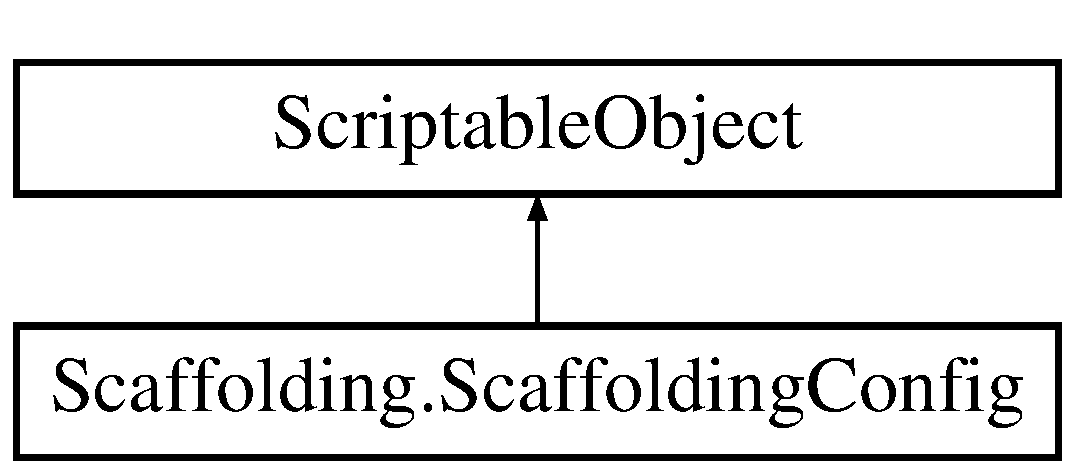
\includegraphics[height=2.000000cm]{class_scaffolding_1_1_scaffolding_config}
\end{center}
\end{figure}
\subsection*{Public Member Functions}
\begin{DoxyCompactItemize}
\item 
\hypertarget{class_scaffolding_1_1_scaffolding_config_acfa863fb89c925a686abc89448070cfd}{Game\+Object {\bfseries Determine\+Parent\+Game\+Object\+Path} ()}\label{class_scaffolding_1_1_scaffolding_config_acfa863fb89c925a686abc89448070cfd}

\item 
\hypertarget{class_scaffolding_1_1_scaffolding_config_aa9921a734611ed4e2257196ea9822628}{Game\+Object {\bfseries Determine\+Parent\+Model\+Game\+Object\+Path} ()}\label{class_scaffolding_1_1_scaffolding_config_aa9921a734611ed4e2257196ea9822628}

\item 
\hypertarget{class_scaffolding_1_1_scaffolding_config_a1da269f9448ac11a2de5d109ef6ff380}{string {\bfseries View\+Prefab\+Path} ()}\label{class_scaffolding_1_1_scaffolding_config_a1da269f9448ac11a2de5d109ef6ff380}

\item 
\hypertarget{class_scaffolding_1_1_scaffolding_config_a5cab51db784ed3e5ad6d03e0e741ba8f}{string {\bfseries Full\+View\+Prefab\+Path} ()}\label{class_scaffolding_1_1_scaffolding_config_a5cab51db784ed3e5ad6d03e0e741ba8f}

\item 
\hypertarget{class_scaffolding_1_1_scaffolding_config_a0086bba5ebde8b4b8bca016b2f6de7fe}{string {\bfseries Scripts\+Path} ()}\label{class_scaffolding_1_1_scaffolding_config_a0086bba5ebde8b4b8bca016b2f6de7fe}

\end{DoxyCompactItemize}
\subsection*{Static Public Member Functions}
\begin{DoxyCompactItemize}
\item 
\hypertarget{class_scaffolding_1_1_scaffolding_config_a3afd16290e0676708bed1189efeffc6e}{static \hyperlink{class_scaffolding_1_1_scaffolding_config}{Scaffolding\+Config} {\bfseries Create\+Instance} ()}\label{class_scaffolding_1_1_scaffolding_config_a3afd16290e0676708bed1189efeffc6e}

\end{DoxyCompactItemize}
\subsection*{Public Attributes}
\begin{DoxyCompactItemize}
\item 
\hypertarget{class_scaffolding_1_1_scaffolding_config_ae0bd7ace4e879759b228509372956b17}{const string {\bfseries V\+I\+E\+W\+\_\+\+N\+A\+M\+E} = \char`\"{}\mbox{[}V\+I\+E\+W\+\_\+\+N\+A\+M\+E\mbox{]}\char`\"{}}\label{class_scaffolding_1_1_scaffolding_config_ae0bd7ace4e879759b228509372956b17}

\item 
\hypertarget{class_scaffolding_1_1_scaffolding_config_a59baee34106272850a7db39b4d6681f4}{const string {\bfseries V\+I\+E\+W\+\_\+\+T\+Y\+P\+E} = \char`\"{}\mbox{[}V\+I\+E\+W\+\_\+\+T\+Y\+P\+E\mbox{]}\char`\"{}}\label{class_scaffolding_1_1_scaffolding_config_a59baee34106272850a7db39b4d6681f4}

\item 
\hypertarget{class_scaffolding_1_1_scaffolding_config_a505921423404d3d4570ba3c4244f85e6}{const string {\bfseries M\+O\+D\+E\+L\+\_\+\+N\+A\+M\+E} = \char`\"{}\mbox{[}M\+O\+D\+E\+L\+\_\+\+N\+A\+M\+E\mbox{]}\char`\"{}}\label{class_scaffolding_1_1_scaffolding_config_a505921423404d3d4570ba3c4244f85e6}

\item 
\hypertarget{class_scaffolding_1_1_scaffolding_config_a7f9a3fa7709f53665a4ec613d2ce73f5}{const string {\bfseries M\+O\+D\+E\+L\+\_\+\+T\+Y\+P\+E} = \char`\"{}\mbox{[}M\+O\+D\+E\+L\+\_\+\+T\+Y\+P\+E\mbox{]}\char`\"{}}\label{class_scaffolding_1_1_scaffolding_config_a7f9a3fa7709f53665a4ec613d2ce73f5}

\item 
\hypertarget{class_scaffolding_1_1_scaffolding_config_a9509e163f79e9cd9fc66b571f47af5c6}{string {\bfseries Scaffolding\+Resources\+Path} = \char`\"{}Assets/Resources/Views/\char`\"{}}\label{class_scaffolding_1_1_scaffolding_config_a9509e163f79e9cd9fc66b571f47af5c6}

\item 
\hypertarget{class_scaffolding_1_1_scaffolding_config_af399dc5b33f5bba471e5caf13b1eeda1}{string {\bfseries Scaffolding\+Scripts\+Path} = \char`\"{}Assets/Scripts/Views/\char`\"{}}\label{class_scaffolding_1_1_scaffolding_config_af399dc5b33f5bba471e5caf13b1eeda1}

\item 
\hypertarget{class_scaffolding_1_1_scaffolding_config_a22bd85373e437aab80656173c4c5a3b0}{string {\bfseries Scaffolding\+Instantiate\+Path} = \char`\"{}Views/\char`\"{}}\label{class_scaffolding_1_1_scaffolding_config_a22bd85373e437aab80656173c4c5a3b0}

\item 
\hypertarget{class_scaffolding_1_1_scaffolding_config_a2ce12de1113d8c1efd370b3d8bdf1b51}{string {\bfseries Scaffolding\+Model\+Instantiate\+Path} = \char`\"{}Model/\char`\"{}}\label{class_scaffolding_1_1_scaffolding_config_a2ce12de1113d8c1efd370b3d8bdf1b51}

\item 
\hypertarget{class_scaffolding_1_1_scaffolding_config_ab77a584978da96b9bed8ee5bcf7884aa}{string {\bfseries Scaffolding\+Path} = \char`\"{}Assets/\char`\"{}}\label{class_scaffolding_1_1_scaffolding_config_ab77a584978da96b9bed8ee5bcf7884aa}

\item 
\hypertarget{class_scaffolding_1_1_scaffolding_config_a2bb653e80aa82c253f3ff1d5c82d9513}{bool {\bfseries Scaffolding\+Enable\+All\+Gameobjects} = true}\label{class_scaffolding_1_1_scaffolding_config_a2bb653e80aa82c253f3ff1d5c82d9513}

\item 
\hypertarget{class_scaffolding_1_1_scaffolding_config_ae94d80ef79bbe1870d5d607571674634}{string {\bfseries Starting\+View}}\label{class_scaffolding_1_1_scaffolding_config_ae94d80ef79bbe1870d5d607571674634}

\item 
\hypertarget{class_scaffolding_1_1_scaffolding_config_aedffba3b54ff1d82e1c4ee39fa3ebec4}{View\+Type {\bfseries Starting\+View\+Type}}\label{class_scaffolding_1_1_scaffolding_config_aedffba3b54ff1d82e1c4ee39fa3ebec4}

\end{DoxyCompactItemize}
\subsection*{Static Public Attributes}
\begin{DoxyCompactItemize}
\item 
\hypertarget{class_scaffolding_1_1_scaffolding_config_a3462d710777d931663953686aa8bb0f6}{static \hyperlink{class_scaffolding_1_1_scaffolding_config}{Scaffolding\+Config} {\bfseries \+\_\+instance}}\label{class_scaffolding_1_1_scaffolding_config_a3462d710777d931663953686aa8bb0f6}

\end{DoxyCompactItemize}
\subsection*{Properties}
\begin{DoxyCompactItemize}
\item 
\hypertarget{class_scaffolding_1_1_scaffolding_config_ae7c97102fe5518cfcdcfd7d440d1f163}{static \hyperlink{class_scaffolding_1_1_scaffolding_config}{Scaffolding\+Config} {\bfseries Instance}\hspace{0.3cm}{\ttfamily  \mbox{[}get\mbox{]}}}\label{class_scaffolding_1_1_scaffolding_config_ae7c97102fe5518cfcdcfd7d440d1f163}

\end{DoxyCompactItemize}


The documentation for this class was generated from the following file\+:\begin{DoxyCompactItemize}
\item 
Extras/Scaffolding\+Config.\+cs\end{DoxyCompactItemize}

\hypertarget{class_scaffolding_1_1_s_object}{\section{Scaffolding.\+S\+Object Class Reference}
\label{class_scaffolding_1_1_s_object}\index{Scaffolding.\+S\+Object@{Scaffolding.\+S\+Object}}
}


Value object. Used for passing data between views. Pack any data you require into this, and On\+Show\+Start can retrieve it.  


\subsection*{Public Member Functions}
\begin{DoxyCompactItemize}
\item 
void \hyperlink{class_scaffolding_1_1_s_object_a85026a282f20ae9319fcbbc8894a0cf0}{Add\+Int} (string key, int value)
\begin{DoxyCompactList}\small\item\em Add an int into the object. \end{DoxyCompactList}\item 
void \hyperlink{class_scaffolding_1_1_s_object_aa6d9e75007547ef7feb0047ae6458edb}{Add\+String} (string key, string value)
\begin{DoxyCompactList}\small\item\em Add a string into the object. \end{DoxyCompactList}\item 
void \hyperlink{class_scaffolding_1_1_s_object_aabbaa83927a45116a89103ddac5d3242}{Add\+Float} (string key, float value)
\begin{DoxyCompactList}\small\item\em Add a float into the object. \end{DoxyCompactList}\item 
void \hyperlink{class_scaffolding_1_1_s_object_a6a595710bc12e94c5c5c696bb0b98b85}{Add\+Bool} (string key, bool value)
\begin{DoxyCompactList}\small\item\em Add a bool into the object. \end{DoxyCompactList}\item 
void \hyperlink{class_scaffolding_1_1_s_object_a3fea64b340f46919191c1bc8acefa0ad}{Add\+Object\+List} (string key, List$<$ System.\+Object $>$ value)
\begin{DoxyCompactList}\small\item\em Add an object list into the object. \end{DoxyCompactList}\item 
void \hyperlink{class_scaffolding_1_1_s_object_ada60ea0906706ebbfc10e04570aafa28}{Add\+Object\+Array} (string key, System.\+Object\mbox{[}$\,$\mbox{]} value)
\begin{DoxyCompactList}\small\item\em Add an object array into the object. \end{DoxyCompactList}\item 
void \hyperlink{class_scaffolding_1_1_s_object_a88d180b12997208394f7c7a5940b67bf}{Add\+Object} (string key, System.\+Object value)
\begin{DoxyCompactList}\small\item\em Add an object into the object. \end{DoxyCompactList}\item 
void \hyperlink{class_scaffolding_1_1_s_object_a21b5f15d73a960dcf8afc7bc7b695d30}{Add\+Action} (string key, System.\+Action value)
\begin{DoxyCompactList}\small\item\em Add an action into the object. \end{DoxyCompactList}\item 
\hypertarget{class_scaffolding_1_1_s_object_a72a6eac036c3a1c8ad2ec2d2ecbcc504}{bool {\bfseries Has\+Key} (string key)}\label{class_scaffolding_1_1_s_object_a72a6eac036c3a1c8ad2ec2d2ecbcc504}

\item 
int \hyperlink{class_scaffolding_1_1_s_object_adbad6746e1fbc0339f6ec2fb650ab6a1}{Get\+Int} (string key)
\begin{DoxyCompactList}\small\item\em Gets the int with Key. \end{DoxyCompactList}\item 
string \hyperlink{class_scaffolding_1_1_s_object_a6c52bfa3a63b544e2b894655f4214455}{Get\+String} (string key)
\begin{DoxyCompactList}\small\item\em Gets the string with Key. \end{DoxyCompactList}\item 
float \hyperlink{class_scaffolding_1_1_s_object_ab72b3f6b94c3a06522d8b2f9c2def605}{Get\+Float} (string key)
\begin{DoxyCompactList}\small\item\em Gets the float with Key. \end{DoxyCompactList}\item 
bool \hyperlink{class_scaffolding_1_1_s_object_a94ad6ed5838a7175ed8b56308366885e}{Get\+Bool} (string key)
\begin{DoxyCompactList}\small\item\em Gets the bool with Key. \end{DoxyCompactList}\item 
List$<$ System.\+Object $>$ \hyperlink{class_scaffolding_1_1_s_object_a4bcc3932ccdbca7def14a51da52cd98c}{Get\+Object\+List} (string key)
\begin{DoxyCompactList}\small\item\em Gets the object list with Key. \end{DoxyCompactList}\item 
System.\+Object\mbox{[}$\,$\mbox{]} \hyperlink{class_scaffolding_1_1_s_object_ac1c6ee446da4c0a8b3f99df78860c36b}{Get\+Object\+Array} (string key)
\begin{DoxyCompactList}\small\item\em Gets the object array with Key. \end{DoxyCompactList}\item 
System.\+Object \hyperlink{class_scaffolding_1_1_s_object_abdbe5a43da1a3eef59d3621584da8804}{Get\+Object} (string key)
\begin{DoxyCompactList}\small\item\em Gets the object with Key. \end{DoxyCompactList}\item 
System.\+Action \hyperlink{class_scaffolding_1_1_s_object_a392574556cb6c4ced6b93e97a74b88a0}{Get\+Action} (string key)
\begin{DoxyCompactList}\small\item\em Gets the action with Key. \end{DoxyCompactList}\end{DoxyCompactItemize}


\subsection{Detailed Description}
Value object. Used for passing data between views. Pack any data you require into this, and On\+Show\+Start can retrieve it. 



\subsection{Member Function Documentation}
\hypertarget{class_scaffolding_1_1_s_object_a21b5f15d73a960dcf8afc7bc7b695d30}{\index{Scaffolding\+::\+S\+Object@{Scaffolding\+::\+S\+Object}!Add\+Action@{Add\+Action}}
\index{Add\+Action@{Add\+Action}!Scaffolding\+::\+S\+Object@{Scaffolding\+::\+S\+Object}}
\subsubsection[{Add\+Action}]{\setlength{\rightskip}{0pt plus 5cm}void Scaffolding.\+S\+Object.\+Add\+Action (
\begin{DoxyParamCaption}
\item[{string}]{key, }
\item[{System.\+Action}]{value}
\end{DoxyParamCaption}
)}}\label{class_scaffolding_1_1_s_object_a21b5f15d73a960dcf8afc7bc7b695d30}


Add an action into the object. 


\begin{DoxyParams}{Parameters}
{\em key} & Key.\\
\hline
{\em value} & Value.\\
\hline
\end{DoxyParams}
\hypertarget{class_scaffolding_1_1_s_object_a6a595710bc12e94c5c5c696bb0b98b85}{\index{Scaffolding\+::\+S\+Object@{Scaffolding\+::\+S\+Object}!Add\+Bool@{Add\+Bool}}
\index{Add\+Bool@{Add\+Bool}!Scaffolding\+::\+S\+Object@{Scaffolding\+::\+S\+Object}}
\subsubsection[{Add\+Bool}]{\setlength{\rightskip}{0pt plus 5cm}void Scaffolding.\+S\+Object.\+Add\+Bool (
\begin{DoxyParamCaption}
\item[{string}]{key, }
\item[{bool}]{value}
\end{DoxyParamCaption}
)}}\label{class_scaffolding_1_1_s_object_a6a595710bc12e94c5c5c696bb0b98b85}


Add a bool into the object. 


\begin{DoxyParams}{Parameters}
{\em key} & Key.\\
\hline
{\em value} & If set to {\ttfamily true} value.\\
\hline
\end{DoxyParams}
\hypertarget{class_scaffolding_1_1_s_object_aabbaa83927a45116a89103ddac5d3242}{\index{Scaffolding\+::\+S\+Object@{Scaffolding\+::\+S\+Object}!Add\+Float@{Add\+Float}}
\index{Add\+Float@{Add\+Float}!Scaffolding\+::\+S\+Object@{Scaffolding\+::\+S\+Object}}
\subsubsection[{Add\+Float}]{\setlength{\rightskip}{0pt plus 5cm}void Scaffolding.\+S\+Object.\+Add\+Float (
\begin{DoxyParamCaption}
\item[{string}]{key, }
\item[{float}]{value}
\end{DoxyParamCaption}
)}}\label{class_scaffolding_1_1_s_object_aabbaa83927a45116a89103ddac5d3242}


Add a float into the object. 


\begin{DoxyParams}{Parameters}
{\em key} & Key.\\
\hline
{\em value} & Value.\\
\hline
\end{DoxyParams}
\hypertarget{class_scaffolding_1_1_s_object_a85026a282f20ae9319fcbbc8894a0cf0}{\index{Scaffolding\+::\+S\+Object@{Scaffolding\+::\+S\+Object}!Add\+Int@{Add\+Int}}
\index{Add\+Int@{Add\+Int}!Scaffolding\+::\+S\+Object@{Scaffolding\+::\+S\+Object}}
\subsubsection[{Add\+Int}]{\setlength{\rightskip}{0pt plus 5cm}void Scaffolding.\+S\+Object.\+Add\+Int (
\begin{DoxyParamCaption}
\item[{string}]{key, }
\item[{int}]{value}
\end{DoxyParamCaption}
)}}\label{class_scaffolding_1_1_s_object_a85026a282f20ae9319fcbbc8894a0cf0}


Add an int into the object. 


\begin{DoxyParams}{Parameters}
{\em key} & Key.\\
\hline
{\em value} & Value.\\
\hline
\end{DoxyParams}
\hypertarget{class_scaffolding_1_1_s_object_a88d180b12997208394f7c7a5940b67bf}{\index{Scaffolding\+::\+S\+Object@{Scaffolding\+::\+S\+Object}!Add\+Object@{Add\+Object}}
\index{Add\+Object@{Add\+Object}!Scaffolding\+::\+S\+Object@{Scaffolding\+::\+S\+Object}}
\subsubsection[{Add\+Object}]{\setlength{\rightskip}{0pt plus 5cm}void Scaffolding.\+S\+Object.\+Add\+Object (
\begin{DoxyParamCaption}
\item[{string}]{key, }
\item[{System.\+Object}]{value}
\end{DoxyParamCaption}
)}}\label{class_scaffolding_1_1_s_object_a88d180b12997208394f7c7a5940b67bf}


Add an object into the object. 


\begin{DoxyParams}{Parameters}
{\em key} & Key.\\
\hline
{\em value} & Value.\\
\hline
\end{DoxyParams}
\hypertarget{class_scaffolding_1_1_s_object_ada60ea0906706ebbfc10e04570aafa28}{\index{Scaffolding\+::\+S\+Object@{Scaffolding\+::\+S\+Object}!Add\+Object\+Array@{Add\+Object\+Array}}
\index{Add\+Object\+Array@{Add\+Object\+Array}!Scaffolding\+::\+S\+Object@{Scaffolding\+::\+S\+Object}}
\subsubsection[{Add\+Object\+Array}]{\setlength{\rightskip}{0pt plus 5cm}void Scaffolding.\+S\+Object.\+Add\+Object\+Array (
\begin{DoxyParamCaption}
\item[{string}]{key, }
\item[{System.\+Object\mbox{[}$\,$\mbox{]}}]{value}
\end{DoxyParamCaption}
)}}\label{class_scaffolding_1_1_s_object_ada60ea0906706ebbfc10e04570aafa28}


Add an object array into the object. 


\begin{DoxyParams}{Parameters}
{\em key} & Key.\\
\hline
{\em value} & Value.\\
\hline
\end{DoxyParams}
\hypertarget{class_scaffolding_1_1_s_object_a3fea64b340f46919191c1bc8acefa0ad}{\index{Scaffolding\+::\+S\+Object@{Scaffolding\+::\+S\+Object}!Add\+Object\+List@{Add\+Object\+List}}
\index{Add\+Object\+List@{Add\+Object\+List}!Scaffolding\+::\+S\+Object@{Scaffolding\+::\+S\+Object}}
\subsubsection[{Add\+Object\+List}]{\setlength{\rightskip}{0pt plus 5cm}void Scaffolding.\+S\+Object.\+Add\+Object\+List (
\begin{DoxyParamCaption}
\item[{string}]{key, }
\item[{List$<$ System.\+Object $>$}]{value}
\end{DoxyParamCaption}
)}}\label{class_scaffolding_1_1_s_object_a3fea64b340f46919191c1bc8acefa0ad}


Add an object list into the object. 


\begin{DoxyParams}{Parameters}
{\em key} & Key.\\
\hline
{\em value} & Value.\\
\hline
\end{DoxyParams}
\hypertarget{class_scaffolding_1_1_s_object_aa6d9e75007547ef7feb0047ae6458edb}{\index{Scaffolding\+::\+S\+Object@{Scaffolding\+::\+S\+Object}!Add\+String@{Add\+String}}
\index{Add\+String@{Add\+String}!Scaffolding\+::\+S\+Object@{Scaffolding\+::\+S\+Object}}
\subsubsection[{Add\+String}]{\setlength{\rightskip}{0pt plus 5cm}void Scaffolding.\+S\+Object.\+Add\+String (
\begin{DoxyParamCaption}
\item[{string}]{key, }
\item[{string}]{value}
\end{DoxyParamCaption}
)}}\label{class_scaffolding_1_1_s_object_aa6d9e75007547ef7feb0047ae6458edb}


Add a string into the object. 


\begin{DoxyParams}{Parameters}
{\em key} & Key.\\
\hline
{\em value} & Value.\\
\hline
\end{DoxyParams}
\hypertarget{class_scaffolding_1_1_s_object_a392574556cb6c4ced6b93e97a74b88a0}{\index{Scaffolding\+::\+S\+Object@{Scaffolding\+::\+S\+Object}!Get\+Action@{Get\+Action}}
\index{Get\+Action@{Get\+Action}!Scaffolding\+::\+S\+Object@{Scaffolding\+::\+S\+Object}}
\subsubsection[{Get\+Action}]{\setlength{\rightskip}{0pt plus 5cm}System.\+Action Scaffolding.\+S\+Object.\+Get\+Action (
\begin{DoxyParamCaption}
\item[{string}]{key}
\end{DoxyParamCaption}
)}}\label{class_scaffolding_1_1_s_object_a392574556cb6c4ced6b93e97a74b88a0}


Gets the action with Key. 

\begin{DoxyReturn}{Returns}
The object.
\end{DoxyReturn}

\begin{DoxyParams}{Parameters}
{\em key} & Key.\\
\hline
\end{DoxyParams}
\hypertarget{class_scaffolding_1_1_s_object_a94ad6ed5838a7175ed8b56308366885e}{\index{Scaffolding\+::\+S\+Object@{Scaffolding\+::\+S\+Object}!Get\+Bool@{Get\+Bool}}
\index{Get\+Bool@{Get\+Bool}!Scaffolding\+::\+S\+Object@{Scaffolding\+::\+S\+Object}}
\subsubsection[{Get\+Bool}]{\setlength{\rightskip}{0pt plus 5cm}bool Scaffolding.\+S\+Object.\+Get\+Bool (
\begin{DoxyParamCaption}
\item[{string}]{key}
\end{DoxyParamCaption}
)}}\label{class_scaffolding_1_1_s_object_a94ad6ed5838a7175ed8b56308366885e}


Gets the bool with Key. 

\begin{DoxyReturn}{Returns}
{\ttfamily true}, if bool was gotten, {\ttfamily false} otherwise.
\end{DoxyReturn}

\begin{DoxyParams}{Parameters}
{\em key} & Key.\\
\hline
\end{DoxyParams}
\hypertarget{class_scaffolding_1_1_s_object_ab72b3f6b94c3a06522d8b2f9c2def605}{\index{Scaffolding\+::\+S\+Object@{Scaffolding\+::\+S\+Object}!Get\+Float@{Get\+Float}}
\index{Get\+Float@{Get\+Float}!Scaffolding\+::\+S\+Object@{Scaffolding\+::\+S\+Object}}
\subsubsection[{Get\+Float}]{\setlength{\rightskip}{0pt plus 5cm}float Scaffolding.\+S\+Object.\+Get\+Float (
\begin{DoxyParamCaption}
\item[{string}]{key}
\end{DoxyParamCaption}
)}}\label{class_scaffolding_1_1_s_object_ab72b3f6b94c3a06522d8b2f9c2def605}


Gets the float with Key. 

\begin{DoxyReturn}{Returns}
The float.
\end{DoxyReturn}

\begin{DoxyParams}{Parameters}
{\em key} & Key.\\
\hline
\end{DoxyParams}
\hypertarget{class_scaffolding_1_1_s_object_adbad6746e1fbc0339f6ec2fb650ab6a1}{\index{Scaffolding\+::\+S\+Object@{Scaffolding\+::\+S\+Object}!Get\+Int@{Get\+Int}}
\index{Get\+Int@{Get\+Int}!Scaffolding\+::\+S\+Object@{Scaffolding\+::\+S\+Object}}
\subsubsection[{Get\+Int}]{\setlength{\rightskip}{0pt plus 5cm}int Scaffolding.\+S\+Object.\+Get\+Int (
\begin{DoxyParamCaption}
\item[{string}]{key}
\end{DoxyParamCaption}
)}}\label{class_scaffolding_1_1_s_object_adbad6746e1fbc0339f6ec2fb650ab6a1}


Gets the int with Key. 

\begin{DoxyReturn}{Returns}
The int.
\end{DoxyReturn}

\begin{DoxyParams}{Parameters}
{\em key} & Key.\\
\hline
\end{DoxyParams}
\hypertarget{class_scaffolding_1_1_s_object_abdbe5a43da1a3eef59d3621584da8804}{\index{Scaffolding\+::\+S\+Object@{Scaffolding\+::\+S\+Object}!Get\+Object@{Get\+Object}}
\index{Get\+Object@{Get\+Object}!Scaffolding\+::\+S\+Object@{Scaffolding\+::\+S\+Object}}
\subsubsection[{Get\+Object}]{\setlength{\rightskip}{0pt plus 5cm}System.\+Object Scaffolding.\+S\+Object.\+Get\+Object (
\begin{DoxyParamCaption}
\item[{string}]{key}
\end{DoxyParamCaption}
)}}\label{class_scaffolding_1_1_s_object_abdbe5a43da1a3eef59d3621584da8804}


Gets the object with Key. 

\begin{DoxyReturn}{Returns}
The object.
\end{DoxyReturn}

\begin{DoxyParams}{Parameters}
{\em key} & Key.\\
\hline
\end{DoxyParams}
\hypertarget{class_scaffolding_1_1_s_object_ac1c6ee446da4c0a8b3f99df78860c36b}{\index{Scaffolding\+::\+S\+Object@{Scaffolding\+::\+S\+Object}!Get\+Object\+Array@{Get\+Object\+Array}}
\index{Get\+Object\+Array@{Get\+Object\+Array}!Scaffolding\+::\+S\+Object@{Scaffolding\+::\+S\+Object}}
\subsubsection[{Get\+Object\+Array}]{\setlength{\rightskip}{0pt plus 5cm}System.\+Object \mbox{[}$\,$\mbox{]} Scaffolding.\+S\+Object.\+Get\+Object\+Array (
\begin{DoxyParamCaption}
\item[{string}]{key}
\end{DoxyParamCaption}
)}}\label{class_scaffolding_1_1_s_object_ac1c6ee446da4c0a8b3f99df78860c36b}


Gets the object array with Key. 

\begin{DoxyReturn}{Returns}
The object array.
\end{DoxyReturn}

\begin{DoxyParams}{Parameters}
{\em key} & Key.\\
\hline
\end{DoxyParams}
\hypertarget{class_scaffolding_1_1_s_object_a4bcc3932ccdbca7def14a51da52cd98c}{\index{Scaffolding\+::\+S\+Object@{Scaffolding\+::\+S\+Object}!Get\+Object\+List@{Get\+Object\+List}}
\index{Get\+Object\+List@{Get\+Object\+List}!Scaffolding\+::\+S\+Object@{Scaffolding\+::\+S\+Object}}
\subsubsection[{Get\+Object\+List}]{\setlength{\rightskip}{0pt plus 5cm}List$<$System.\+Object$>$ Scaffolding.\+S\+Object.\+Get\+Object\+List (
\begin{DoxyParamCaption}
\item[{string}]{key}
\end{DoxyParamCaption}
)}}\label{class_scaffolding_1_1_s_object_a4bcc3932ccdbca7def14a51da52cd98c}


Gets the object list with Key. 

\begin{DoxyReturn}{Returns}
The object list.
\end{DoxyReturn}

\begin{DoxyParams}{Parameters}
{\em key} & Key.\\
\hline
\end{DoxyParams}
\hypertarget{class_scaffolding_1_1_s_object_a6c52bfa3a63b544e2b894655f4214455}{\index{Scaffolding\+::\+S\+Object@{Scaffolding\+::\+S\+Object}!Get\+String@{Get\+String}}
\index{Get\+String@{Get\+String}!Scaffolding\+::\+S\+Object@{Scaffolding\+::\+S\+Object}}
\subsubsection[{Get\+String}]{\setlength{\rightskip}{0pt plus 5cm}string Scaffolding.\+S\+Object.\+Get\+String (
\begin{DoxyParamCaption}
\item[{string}]{key}
\end{DoxyParamCaption}
)}}\label{class_scaffolding_1_1_s_object_a6c52bfa3a63b544e2b894655f4214455}


Gets the string with Key. 

\begin{DoxyReturn}{Returns}
The string.
\end{DoxyReturn}

\begin{DoxyParams}{Parameters}
{\em key} & Key.\\
\hline
\end{DoxyParams}


The documentation for this class was generated from the following file\+:\begin{DoxyCompactItemize}
\item 
Extras/S\+Object.\+cs\end{DoxyCompactItemize}

\hypertarget{class_scaffolding_1_1_swipe_input}{\section{Scaffolding.\+Swipe\+Input Class Reference}
\label{class_scaffolding_1_1_swipe_input}\index{Scaffolding.\+Swipe\+Input@{Scaffolding.\+Swipe\+Input}}
}


Swipe input replicates the swipe gesture and dispatches a callback for a chosen swipe direction.  


Inheritance diagram for Scaffolding.\+Swipe\+Input\+:\begin{figure}[H]
\begin{center}
\leavevmode
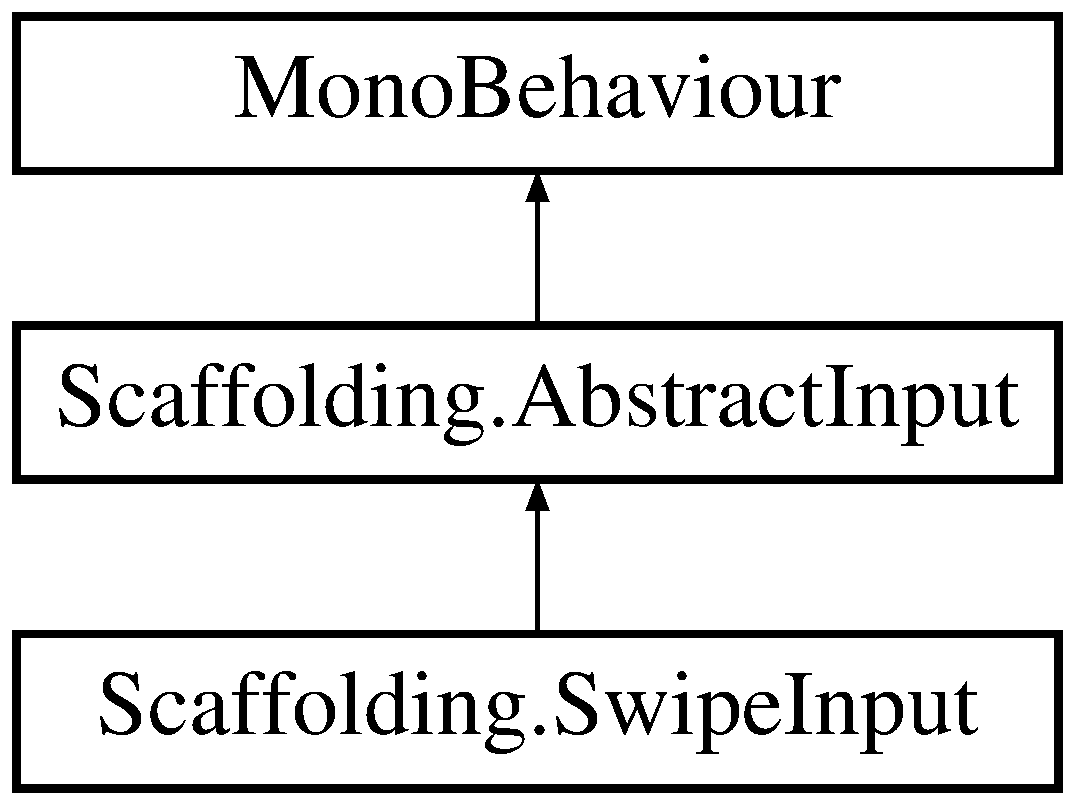
\includegraphics[height=3.000000cm]{class_scaffolding_1_1_swipe_input}
\end{center}
\end{figure}
\subsection*{Public Member Functions}
\begin{DoxyCompactItemize}
\item 
override void \hyperlink{class_scaffolding_1_1_swipe_input_a5d19c1744df90f14d150241605cb86bf}{Cleanup} ()
\begin{DoxyCompactList}\small\item\em The inputs clean up phase. \end{DoxyCompactList}\item 
void \hyperlink{class_scaffolding_1_1_swipe_input_a00ad2fde21a1aa47c4dbfa36768a0bc3}{Register\+Swipe\+Callback} (Action$<$ Swipe\+Direction $>$ callback)
\begin{DoxyCompactList}\small\item\em Register a callback handler fo the swipe input. \end{DoxyCompactList}\item 
override void \hyperlink{class_scaffolding_1_1_swipe_input_a818aba4106a64b5dde4977bca4b358a7}{Handle\+Event\+Dragged} (\hyperlink{class_scaffolding_1_1_input_tracker}{Input\+Tracker} tracker)
\begin{DoxyCompactList}\small\item\em Event\+Dragged, dispatched by Scaffoldings \hyperlink{class_scaffolding_1_1_input_manager}{Input\+Manager} Passes through a \hyperlink{class_scaffolding_1_1_input_tracker}{Input\+Tracker} of the current touch. \end{DoxyCompactList}\end{DoxyCompactItemize}
\subsection*{Public Attributes}
\begin{DoxyCompactItemize}
\item 
\hypertarget{class_scaffolding_1_1_swipe_input_a96c9d39a58afb3717925a4c9a0347791}{float {\bfseries velocity\+Threshold}}\label{class_scaffolding_1_1_swipe_input_a96c9d39a58afb3717925a4c9a0347791}

\end{DoxyCompactItemize}


\subsection{Detailed Description}
Swipe input replicates the swipe gesture and dispatches a callback for a chosen swipe direction. 



\subsection{Member Function Documentation}
\hypertarget{class_scaffolding_1_1_swipe_input_a5d19c1744df90f14d150241605cb86bf}{\index{Scaffolding\+::\+Swipe\+Input@{Scaffolding\+::\+Swipe\+Input}!Cleanup@{Cleanup}}
\index{Cleanup@{Cleanup}!Scaffolding\+::\+Swipe\+Input@{Scaffolding\+::\+Swipe\+Input}}
\subsubsection[{Cleanup}]{\setlength{\rightskip}{0pt plus 5cm}override void Scaffolding.\+Swipe\+Input.\+Cleanup (
\begin{DoxyParamCaption}
{}
\end{DoxyParamCaption}
)\hspace{0.3cm}{\ttfamily [virtual]}}}\label{class_scaffolding_1_1_swipe_input_a5d19c1744df90f14d150241605cb86bf}


The inputs clean up phase. 



Reimplemented from \hyperlink{class_scaffolding_1_1_abstract_input_ab179ae99e76c6c934a0dcba4fc195e68}{Scaffolding.\+Abstract\+Input}.

\hypertarget{class_scaffolding_1_1_swipe_input_a818aba4106a64b5dde4977bca4b358a7}{\index{Scaffolding\+::\+Swipe\+Input@{Scaffolding\+::\+Swipe\+Input}!Handle\+Event\+Dragged@{Handle\+Event\+Dragged}}
\index{Handle\+Event\+Dragged@{Handle\+Event\+Dragged}!Scaffolding\+::\+Swipe\+Input@{Scaffolding\+::\+Swipe\+Input}}
\subsubsection[{Handle\+Event\+Dragged}]{\setlength{\rightskip}{0pt plus 5cm}override void Scaffolding.\+Swipe\+Input.\+Handle\+Event\+Dragged (
\begin{DoxyParamCaption}
\item[{{\bf Input\+Tracker}}]{tracker}
\end{DoxyParamCaption}
)\hspace{0.3cm}{\ttfamily [virtual]}}}\label{class_scaffolding_1_1_swipe_input_a818aba4106a64b5dde4977bca4b358a7}


Event\+Dragged, dispatched by Scaffoldings \hyperlink{class_scaffolding_1_1_input_manager}{Input\+Manager} Passes through a \hyperlink{class_scaffolding_1_1_input_tracker}{Input\+Tracker} of the current touch. 


\begin{DoxyParams}{Parameters}
{\em tracker} & Tracker.\\
\hline
\end{DoxyParams}


Reimplemented from \hyperlink{class_scaffolding_1_1_abstract_input_a5996b0cb611a384e527ce871b9607858}{Scaffolding.\+Abstract\+Input}.

\hypertarget{class_scaffolding_1_1_swipe_input_a00ad2fde21a1aa47c4dbfa36768a0bc3}{\index{Scaffolding\+::\+Swipe\+Input@{Scaffolding\+::\+Swipe\+Input}!Register\+Swipe\+Callback@{Register\+Swipe\+Callback}}
\index{Register\+Swipe\+Callback@{Register\+Swipe\+Callback}!Scaffolding\+::\+Swipe\+Input@{Scaffolding\+::\+Swipe\+Input}}
\subsubsection[{Register\+Swipe\+Callback}]{\setlength{\rightskip}{0pt plus 5cm}void Scaffolding.\+Swipe\+Input.\+Register\+Swipe\+Callback (
\begin{DoxyParamCaption}
\item[{Action$<$ Swipe\+Direction $>$}]{callback}
\end{DoxyParamCaption}
)}}\label{class_scaffolding_1_1_swipe_input_a00ad2fde21a1aa47c4dbfa36768a0bc3}


Register a callback handler fo the swipe input. 

Example\+: public void My\+Callback\+Function(\+Swipe\+Direction direction) \{ //do swipe based code here... \}

\+\_\+swipe\+Input.\+Register\+Swipe\+Callback(\+My\+Callback\+Function);


\begin{DoxyParams}{Parameters}
{\em callback} & Callback.\\
\hline
\end{DoxyParams}


The documentation for this class was generated from the following file\+:\begin{DoxyCompactItemize}
\item 
Input/\+Items/Swipe\+Input.\+cs\end{DoxyCompactItemize}

\hypertarget{class_scaffolding_1_1_view_manager}{\section{Scaffolding.\+View\+Manager Class Reference}
\label{class_scaffolding_1_1_view_manager}\index{Scaffolding.\+View\+Manager@{Scaffolding.\+View\+Manager}}
}
Inheritance diagram for Scaffolding.\+View\+Manager\+:\begin{figure}[H]
\begin{center}
\leavevmode
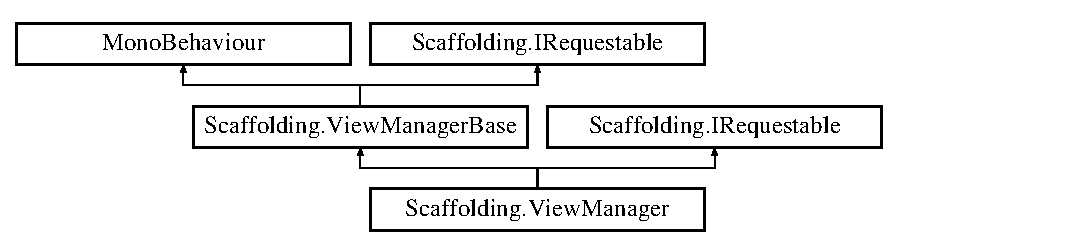
\includegraphics[height=2.871795cm]{class_scaffolding_1_1_view_manager}
\end{center}
\end{figure}
\subsection*{Public Member Functions}
\begin{DoxyCompactItemize}
\item 
Action \hyperlink{class_scaffolding_1_1_view_manager_a8b9e5f3a4043a28c2b7d123724ae87b4}{Override\+Startup\+Sequence} ()
\begin{DoxyCompactList}\small\item\em Overrides the startup sequence. \end{DoxyCompactList}\item 
void \hyperlink{class_scaffolding_1_1_view_manager_a8da654dc78dfd8839c7680315bedd382}{Init} ()
\begin{DoxyCompactList}\small\item\em The startup sequence. \hyperlink{namespace_scaffolding}{Scaffolding} starts from here. \end{DoxyCompactList}\item 
Dictionary$<$ Type, \hyperlink{class_scaffolding_1_1_abstract_view}{Abstract\+View} $>$ \hyperlink{class_scaffolding_1_1_view_manager_a5674ccdc20f2afe33e0f55838fc05f27}{Get\+Current\+Overlays} ()
\begin{DoxyCompactList}\small\item\em Gets the current overlays. \end{DoxyCompactList}\item 
bool \hyperlink{class_scaffolding_1_1_view_manager_a92a53e48d3ba9701d471f52baeb1f98d}{Is\+Overlay\+Showing$<$ T $>$} ()
\begin{DoxyCompactList}\small\item\em Determines whether this instance of the overlay is showing. \end{DoxyCompactList}\item 
\hypertarget{class_scaffolding_1_1_view_manager_a49df4475ef01fb584d6c67df641763a9}{bool {\bfseries Is\+Overlay\+Showing} (Type view)}\label{class_scaffolding_1_1_view_manager_a49df4475ef01fb584d6c67df641763a9}

\item 
bool \hyperlink{class_scaffolding_1_1_view_manager_a85f6fe3eff8b8fabfc846ba3fc109a4a}{Is\+View\+An\+Overlay} (Type type)
\begin{DoxyCompactList}\small\item\em Determines whether the type is an overlay. \end{DoxyCompactList}\item 
\hypertarget{class_scaffolding_1_1_view_manager_a25c9e93c61fcdc0ace620525239d1e5f}{bool {\bfseries Is\+View\+Showing$<$ T $>$} ()}\label{class_scaffolding_1_1_view_manager_a25c9e93c61fcdc0ace620525239d1e5f}

\item 
\hypertarget{class_scaffolding_1_1_view_manager_ac884bcebbcf2c931725299e56e37e2da}{bool {\bfseries Is\+View\+Showing} (Type view)}\label{class_scaffolding_1_1_view_manager_ac884bcebbcf2c931725299e56e37e2da}

\end{DoxyCompactItemize}
\subsection*{Protected Member Functions}
\begin{DoxyCompactItemize}
\item 
\hypertarget{class_scaffolding_1_1_view_manager_a20eef73a9db449ba636716b8381ea282}{void {\bfseries Start} ()}\label{class_scaffolding_1_1_view_manager_a20eef73a9db449ba636716b8381ea282}

\end{DoxyCompactItemize}
\subsection*{Properties}
\begin{DoxyCompactItemize}
\item 
\hyperlink{class_scaffolding_1_1_abstract_view}{Abstract\+View} \hyperlink{class_scaffolding_1_1_view_manager_ac4d88a4e3c77abab903d16959b45cdae}{Last\+Screen}\hspace{0.3cm}{\ttfamily  \mbox{[}get\mbox{]}}
\begin{DoxyCompactList}\small\item\em Gets the last Screen. \end{DoxyCompactList}\item 
\hyperlink{class_scaffolding_1_1_abstract_view}{Abstract\+View} \hyperlink{class_scaffolding_1_1_view_manager_aeba5a2db8a3551991c2be765ee700dbd}{Current\+Screen}\hspace{0.3cm}{\ttfamily  \mbox{[}get\mbox{]}}
\begin{DoxyCompactList}\small\item\em Gets the current screen. \end{DoxyCompactList}\item 
\hyperlink{class_scaffolding_1_1_abstract_view}{Abstract\+View} \hyperlink{class_scaffolding_1_1_view_manager_ad77b108adca50eb2af05eb2dbbe13701}{Target\+Screen}\hspace{0.3cm}{\ttfamily  \mbox{[}get\mbox{]}}
\begin{DoxyCompactList}\small\item\em Gets the target screen. \end{DoxyCompactList}\end{DoxyCompactItemize}
\subsection*{Additional Inherited Members}


\subsection{Member Function Documentation}
\hypertarget{class_scaffolding_1_1_view_manager_a5674ccdc20f2afe33e0f55838fc05f27}{\index{Scaffolding\+::\+View\+Manager@{Scaffolding\+::\+View\+Manager}!Get\+Current\+Overlays@{Get\+Current\+Overlays}}
\index{Get\+Current\+Overlays@{Get\+Current\+Overlays}!Scaffolding\+::\+View\+Manager@{Scaffolding\+::\+View\+Manager}}
\subsubsection[{Get\+Current\+Overlays}]{\setlength{\rightskip}{0pt plus 5cm}Dictionary$<$Type,{\bf Abstract\+View}$>$ Scaffolding.\+View\+Manager.\+Get\+Current\+Overlays (
\begin{DoxyParamCaption}
{}
\end{DoxyParamCaption}
)}}\label{class_scaffolding_1_1_view_manager_a5674ccdc20f2afe33e0f55838fc05f27}


Gets the current overlays. 

\begin{DoxyReturn}{Returns}
The current overlays.
\end{DoxyReturn}
\hypertarget{class_scaffolding_1_1_view_manager_a8da654dc78dfd8839c7680315bedd382}{\index{Scaffolding\+::\+View\+Manager@{Scaffolding\+::\+View\+Manager}!Init@{Init}}
\index{Init@{Init}!Scaffolding\+::\+View\+Manager@{Scaffolding\+::\+View\+Manager}}
\subsubsection[{Init}]{\setlength{\rightskip}{0pt plus 5cm}void Scaffolding.\+View\+Manager.\+Init (
\begin{DoxyParamCaption}
{}
\end{DoxyParamCaption}
)}}\label{class_scaffolding_1_1_view_manager_a8da654dc78dfd8839c7680315bedd382}


The startup sequence. \hyperlink{namespace_scaffolding}{Scaffolding} starts from here. 

\hypertarget{class_scaffolding_1_1_view_manager_a92a53e48d3ba9701d471f52baeb1f98d}{\index{Scaffolding\+::\+View\+Manager@{Scaffolding\+::\+View\+Manager}!Is\+Overlay\+Showing$<$ T $>$@{Is\+Overlay\+Showing$<$ T $>$}}
\index{Is\+Overlay\+Showing$<$ T $>$@{Is\+Overlay\+Showing$<$ T $>$}!Scaffolding\+::\+View\+Manager@{Scaffolding\+::\+View\+Manager}}
\subsubsection[{Is\+Overlay\+Showing$<$ T $>$}]{\setlength{\rightskip}{0pt plus 5cm}bool Scaffolding.\+View\+Manager.\+Is\+Overlay\+Showing$<$ T $>$ (
\begin{DoxyParamCaption}
{}
\end{DoxyParamCaption}
)}}\label{class_scaffolding_1_1_view_manager_a92a53e48d3ba9701d471f52baeb1f98d}


Determines whether this instance of the overlay is showing. 

\begin{DoxyReturn}{Returns}
{\ttfamily true} if this instance is overlay showing; otherwise, {\ttfamily false}.
\end{DoxyReturn}

\begin{DoxyTemplParams}{Template Parameters}
{\em T} & The 1st type parameter.\\
\hline
\end{DoxyTemplParams}
\begin{Desc}
\item[Type Constraints]\begin{description}
\item[{\em T} : {\em Abstract\+View}]\end{description}
\end{Desc}
\hypertarget{class_scaffolding_1_1_view_manager_a85f6fe3eff8b8fabfc846ba3fc109a4a}{\index{Scaffolding\+::\+View\+Manager@{Scaffolding\+::\+View\+Manager}!Is\+View\+An\+Overlay@{Is\+View\+An\+Overlay}}
\index{Is\+View\+An\+Overlay@{Is\+View\+An\+Overlay}!Scaffolding\+::\+View\+Manager@{Scaffolding\+::\+View\+Manager}}
\subsubsection[{Is\+View\+An\+Overlay}]{\setlength{\rightskip}{0pt plus 5cm}bool Scaffolding.\+View\+Manager.\+Is\+View\+An\+Overlay (
\begin{DoxyParamCaption}
\item[{Type}]{type}
\end{DoxyParamCaption}
)}}\label{class_scaffolding_1_1_view_manager_a85f6fe3eff8b8fabfc846ba3fc109a4a}


Determines whether the type is an overlay. 

\begin{DoxyReturn}{Returns}
{\ttfamily true} if the type is an overlay, otherwise; {\ttfamily false}.
\end{DoxyReturn}

\begin{DoxyParams}{Parameters}
{\em type} & Type.\\
\hline
\end{DoxyParams}
\hypertarget{class_scaffolding_1_1_view_manager_a8b9e5f3a4043a28c2b7d123724ae87b4}{\index{Scaffolding\+::\+View\+Manager@{Scaffolding\+::\+View\+Manager}!Override\+Startup\+Sequence@{Override\+Startup\+Sequence}}
\index{Override\+Startup\+Sequence@{Override\+Startup\+Sequence}!Scaffolding\+::\+View\+Manager@{Scaffolding\+::\+View\+Manager}}
\subsubsection[{Override\+Startup\+Sequence}]{\setlength{\rightskip}{0pt plus 5cm}Action Scaffolding.\+View\+Manager.\+Override\+Startup\+Sequence (
\begin{DoxyParamCaption}
{}
\end{DoxyParamCaption}
)}}\label{class_scaffolding_1_1_view_manager_a8b9e5f3a4043a28c2b7d123724ae87b4}


Overrides the startup sequence. 

\begin{DoxyReturn}{Returns}
The callback to contiue the startup sequence when you are finished.
\end{DoxyReturn}


\subsection{Property Documentation}
\hypertarget{class_scaffolding_1_1_view_manager_aeba5a2db8a3551991c2be765ee700dbd}{\index{Scaffolding\+::\+View\+Manager@{Scaffolding\+::\+View\+Manager}!Current\+Screen@{Current\+Screen}}
\index{Current\+Screen@{Current\+Screen}!Scaffolding\+::\+View\+Manager@{Scaffolding\+::\+View\+Manager}}
\subsubsection[{Current\+Screen}]{\setlength{\rightskip}{0pt plus 5cm}{\bf Abstract\+View} Scaffolding.\+View\+Manager.\+Current\+Screen\hspace{0.3cm}{\ttfamily [get]}}}\label{class_scaffolding_1_1_view_manager_aeba5a2db8a3551991c2be765ee700dbd}


Gets the current screen. 

The current screen.\hypertarget{class_scaffolding_1_1_view_manager_ac4d88a4e3c77abab903d16959b45cdae}{\index{Scaffolding\+::\+View\+Manager@{Scaffolding\+::\+View\+Manager}!Last\+Screen@{Last\+Screen}}
\index{Last\+Screen@{Last\+Screen}!Scaffolding\+::\+View\+Manager@{Scaffolding\+::\+View\+Manager}}
\subsubsection[{Last\+Screen}]{\setlength{\rightskip}{0pt plus 5cm}{\bf Abstract\+View} Scaffolding.\+View\+Manager.\+Last\+Screen\hspace{0.3cm}{\ttfamily [get]}}}\label{class_scaffolding_1_1_view_manager_ac4d88a4e3c77abab903d16959b45cdae}


Gets the last Screen. 

The last Screen.\hypertarget{class_scaffolding_1_1_view_manager_ad77b108adca50eb2af05eb2dbbe13701}{\index{Scaffolding\+::\+View\+Manager@{Scaffolding\+::\+View\+Manager}!Target\+Screen@{Target\+Screen}}
\index{Target\+Screen@{Target\+Screen}!Scaffolding\+::\+View\+Manager@{Scaffolding\+::\+View\+Manager}}
\subsubsection[{Target\+Screen}]{\setlength{\rightskip}{0pt plus 5cm}{\bf Abstract\+View} Scaffolding.\+View\+Manager.\+Target\+Screen\hspace{0.3cm}{\ttfamily [get]}}}\label{class_scaffolding_1_1_view_manager_ad77b108adca50eb2af05eb2dbbe13701}


Gets the target screen. 

The target screen.

The documentation for this class was generated from the following file\+:\begin{DoxyCompactItemize}
\item 
Views/View\+Manager.\+cs\end{DoxyCompactItemize}

\hypertarget{class_scaffolding_1_1_view_manager_base}{\section{Scaffolding.\+View\+Manager\+Base Class Reference}
\label{class_scaffolding_1_1_view_manager_base}\index{Scaffolding.\+View\+Manager\+Base@{Scaffolding.\+View\+Manager\+Base}}
}
Inheritance diagram for Scaffolding.\+View\+Manager\+Base\+:\begin{figure}[H]
\begin{center}
\leavevmode
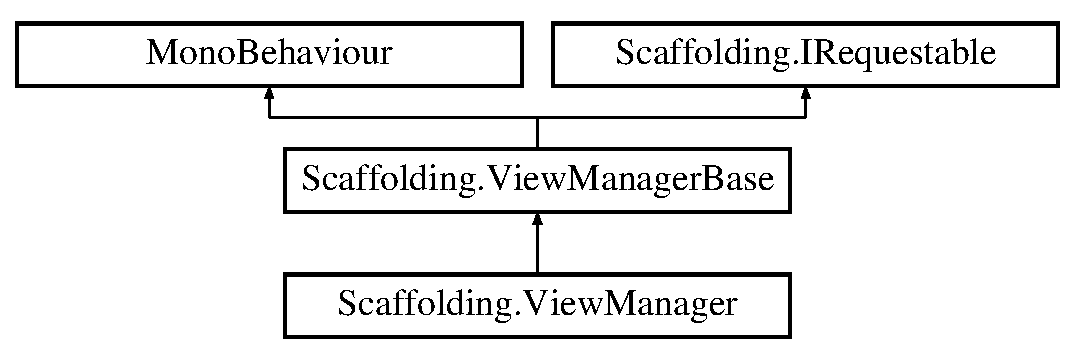
\includegraphics[height=3.000000cm]{class_scaffolding_1_1_view_manager_base}
\end{center}
\end{figure}
\subsection*{Public Member Functions}
\begin{DoxyCompactItemize}
\item 
\hypertarget{class_scaffolding_1_1_view_manager_base_ad47faade879ba9cfe1624960d0a48e25}{delegate void {\bfseries View\+Manager\+Event} (\hyperlink{class_scaffolding_1_1_abstract_view}{Abstract\+View} changed\+View)}\label{class_scaffolding_1_1_view_manager_base_ad47faade879ba9cfe1624960d0a48e25}

\item 
\hypertarget{class_scaffolding_1_1_view_manager_base_a178a05fc2bb3a02de223a09def5d9efc}{void {\bfseries Add\+Animation\+Event\+To\+Transition} (Type target\+View, Animation\+Clip clip, string event\+Name)}\label{class_scaffolding_1_1_view_manager_base_a178a05fc2bb3a02de223a09def5d9efc}

\item 
void \hyperlink{class_scaffolding_1_1_view_manager_base_a3afde7ee1eb394797bba9d334e85cd6e}{Request\+View$<$ T $>$} ()
\begin{DoxyCompactList}\small\item\em Requests the screen to open. \end{DoxyCompactList}\item 
void \hyperlink{class_scaffolding_1_1_view_manager_base_a9707174312efe777211b7ade13cf9ce4}{Request\+View} (Type screen\+Type)
\begin{DoxyCompactList}\small\item\em Requests the screen to open. \end{DoxyCompactList}\item 
void \hyperlink{class_scaffolding_1_1_view_manager_base_a367f6c39d23aa731eb747bb0b9fc0b67}{Request\+View\+With\+Loading\+Overlay$<$ T, L $>$} ()
\begin{DoxyCompactList}\small\item\em Requests the view with a loading view. This is useful if the screen you are moving to is very heavy and takes a long time to load. You can open an overlay to mask this loading while you wait. Once the loading is complete, the overlay will close. \end{DoxyCompactList}\item 
void \hyperlink{class_scaffolding_1_1_view_manager_base_ae56fe5f11df7c468d9a99938b0757e45}{Request\+View\+With\+Loading\+Overlay} (Type screen\+Type, Type loading\+View\+Type)
\begin{DoxyCompactList}\small\item\em Requests the view with a loading view. This is useful if the screen you are moving to is very heavy and takes a long time to load. You can open an overlay to mask this loading while you wait. Once the loading is complete, the overlay will close. \end{DoxyCompactList}\item 
void \hyperlink{class_scaffolding_1_1_view_manager_base_a3afa59b6a26b3aab4f2e426cc9b827c3}{Request\+View\+With\+Loading\+Overlay$<$ T, L $>$} (\hyperlink{class_scaffolding_1_1_s_object}{S\+Object} view\+Data)
\begin{DoxyCompactList}\small\item\em Requests the view with a loading view. This is useful if the screen you are moving to is very heavy and takes a long time to load. You can open an overlay to mask this loading while you wait. Once the loading is complete, the overlay will close. \end{DoxyCompactList}\item 
void \hyperlink{class_scaffolding_1_1_view_manager_base_aa9f6af665d066471cac654181edcf4fe}{Request\+View\+With\+Loading\+Overlay} (Type screen\+Type, Type loading\+View\+Type, \hyperlink{class_scaffolding_1_1_s_object}{S\+Object} view\+Data)
\begin{DoxyCompactList}\small\item\em Requests the view with a loading view. This is useful if the screen you are moving to is very heavy and takes a long time to load. You can open an overlay to mask this loading while you wait. Once the loading is complete, the overlay will close. \end{DoxyCompactList}\item 
void \hyperlink{class_scaffolding_1_1_view_manager_base_ac1e312060187e1b0995b5944145eca4f}{Request\+View$<$ T $>$} (\hyperlink{class_scaffolding_1_1_s_object}{S\+Object} view\+Data)
\begin{DoxyCompactList}\small\item\em Requests the screen with data. \end{DoxyCompactList}\item 
void \hyperlink{class_scaffolding_1_1_view_manager_base_a5e2c66cf402ef8b9f3d8aa1162b06995}{Request\+Force\+Reopen\+View$<$ T $>$} ()
\begin{DoxyCompactList}\small\item\em Request to reopen an already open view \end{DoxyCompactList}\item 
void \hyperlink{class_scaffolding_1_1_view_manager_base_a78c0b2e1361d4962c6cea7c4b983d7ec}{Request\+Force\+Reopen\+View} (Type screen\+Type)
\begin{DoxyCompactList}\small\item\em Request to reopen an already open view \end{DoxyCompactList}\item 
void \hyperlink{class_scaffolding_1_1_view_manager_base_aa28101b866360aae9efceea950535ec6}{Request\+Force\+Reopen\+View$<$ T $>$} (\hyperlink{class_scaffolding_1_1_s_object}{S\+Object} view\+Data)
\begin{DoxyCompactList}\small\item\em Request to reopen an already open view \end{DoxyCompactList}\item 
void \hyperlink{class_scaffolding_1_1_view_manager_base_a950c3fa25288d34a615c8a9b80177b48}{Request\+Force\+Reopen\+View} (Type screen\+Type, \hyperlink{class_scaffolding_1_1_s_object}{S\+Object} view\+Data)
\begin{DoxyCompactList}\small\item\em Request to reopen an already open view \end{DoxyCompactList}\item 
void \hyperlink{class_scaffolding_1_1_view_manager_base_a194a6730d30f15d9cd2bc0809ecbdea7}{Request\+View} (Type screen\+Type, \hyperlink{class_scaffolding_1_1_s_object}{S\+Object} data)
\begin{DoxyCompactList}\small\item\em Requests the screen with data. \end{DoxyCompactList}\item 
void \hyperlink{class_scaffolding_1_1_view_manager_base_a38479b74a1e0cdcfa81f967c753062fb}{Request\+Overlay} (Type overlay\+Type)
\begin{DoxyCompactList}\small\item\em Requests an overlay to open \end{DoxyCompactList}\item 
void \hyperlink{class_scaffolding_1_1_view_manager_base_a8e99066d44cc24df5a78ce9cfa5f792c}{Request\+Overlay$<$ T $>$} ()
\begin{DoxyCompactList}\small\item\em Requests an overlay to open \end{DoxyCompactList}\item 
void \hyperlink{class_scaffolding_1_1_view_manager_base_a8e0638cb6ce962d9f6b4accf70399eca}{Request\+Overlay$<$ T $>$} (\hyperlink{class_scaffolding_1_1_s_object}{S\+Object} view\+Data)
\begin{DoxyCompactList}\small\item\em Requests an overlay to open \end{DoxyCompactList}\item 
void \hyperlink{class_scaffolding_1_1_view_manager_base_ac22aa52e9532ff847d464a251082dce3}{Request\+Overlay} (Type overlay\+Type, \hyperlink{class_scaffolding_1_1_s_object}{S\+Object} view\+Data)
\begin{DoxyCompactList}\small\item\em Requests the overlay open with data. \end{DoxyCompactList}\item 
void \hyperlink{class_scaffolding_1_1_view_manager_base_afe33255e871d0c4228c7629911e97df2}{Request\+Overlay\+Close$<$ T $>$} ()
\begin{DoxyCompactList}\small\item\em Requests the overlay to close \end{DoxyCompactList}\item 
void \hyperlink{class_scaffolding_1_1_view_manager_base_a9fd519e341f2075813bfb900a461130d}{Request\+Overlay\+Close} (Type overlay\+Type)
\begin{DoxyCompactList}\small\item\em Requests the overlay to close \end{DoxyCompactList}\item 
void \hyperlink{class_scaffolding_1_1_view_manager_base_a187a7e1d15142349f697174cf8f868b4}{Request\+Overlay\+Force\+Close$<$ T $>$} ()
\begin{DoxyCompactList}\small\item\em Requests the overlay to force close. This will skip the Hide\+Start() method of the target overlay. \end{DoxyCompactList}\item 
void \hyperlink{class_scaffolding_1_1_view_manager_base_a1f2666a080551b586f7f0847f3958e5d}{Request\+Overlay\+Force\+Close} (Type overlay\+Type)
\begin{DoxyCompactList}\small\item\em Requests the overlay to force close. This will skip the Hide\+Start() method of the target overlay. \end{DoxyCompactList}\item 
void \hyperlink{class_scaffolding_1_1_view_manager_base_a3adaf70659846c8ba4fe29c6d145ca3e}{Request\+Overlay\+Close\+All} ()
\begin{DoxyCompactList}\small\item\em Requests all open overlays to close. \end{DoxyCompactList}\item 
void \hyperlink{class_scaffolding_1_1_view_manager_base_a85021ea2e970c2e46badb5bdf17cbf49}{Request\+Overlay\+Force\+Close\+All} ()
\begin{DoxyCompactList}\small\item\em Requests all open overlays to be forced close. \end{DoxyCompactList}\item 
\hypertarget{class_scaffolding_1_1_view_manager_base_aa255a6fa1922a757dbc52f66e3cd75f6}{void {\bfseries Register\+View\+To\+Model} (\hyperlink{class_scaffolding_1_1_abstract_view}{Abstract\+View} view, \hyperlink{class_scaffolding_1_1_abstract_model}{Abstract\+Model} model)}\label{class_scaffolding_1_1_view_manager_base_aa255a6fa1922a757dbc52f66e3cd75f6}

\item 
\hypertarget{class_scaffolding_1_1_view_manager_base_a9b5acbdc66d3036270f2cc22c5c6bfb4}{void {\bfseries Un\+Register\+View\+From\+Model} (\hyperlink{class_scaffolding_1_1_abstract_view}{Abstract\+View} view)}\label{class_scaffolding_1_1_view_manager_base_a9b5acbdc66d3036270f2cc22c5c6bfb4}

\end{DoxyCompactItemize}
\subsection*{Events}
\begin{DoxyCompactItemize}
\item 
\hypertarget{class_scaffolding_1_1_view_manager_base_af6f41b20382ba5d9bca9c52485c4fe48}{static View\+Manager\+Event {\bfseries View\+Opened}}\label{class_scaffolding_1_1_view_manager_base_af6f41b20382ba5d9bca9c52485c4fe48}

\item 
\hypertarget{class_scaffolding_1_1_view_manager_base_a18ce0bb6faba2bd7137c5fdef3652040}{static View\+Manager\+Event {\bfseries View\+Closed}}\label{class_scaffolding_1_1_view_manager_base_a18ce0bb6faba2bd7137c5fdef3652040}

\item 
\hypertarget{class_scaffolding_1_1_view_manager_base_a4bf89b7b4b2c4243880c87d1eed8a7d2}{static View\+Manager\+Event {\bfseries Overlay\+Opened}}\label{class_scaffolding_1_1_view_manager_base_a4bf89b7b4b2c4243880c87d1eed8a7d2}

\item 
\hypertarget{class_scaffolding_1_1_view_manager_base_a86066209ff5b3b786cd3bc926acabe4e}{static View\+Manager\+Event {\bfseries Overlay\+Closed}}\label{class_scaffolding_1_1_view_manager_base_a86066209ff5b3b786cd3bc926acabe4e}

\end{DoxyCompactItemize}


\subsection{Member Function Documentation}
\hypertarget{class_scaffolding_1_1_view_manager_base_a78c0b2e1361d4962c6cea7c4b983d7ec}{\index{Scaffolding\+::\+View\+Manager\+Base@{Scaffolding\+::\+View\+Manager\+Base}!Request\+Force\+Reopen\+View@{Request\+Force\+Reopen\+View}}
\index{Request\+Force\+Reopen\+View@{Request\+Force\+Reopen\+View}!Scaffolding\+::\+View\+Manager\+Base@{Scaffolding\+::\+View\+Manager\+Base}}
\subsubsection[{Request\+Force\+Reopen\+View}]{\setlength{\rightskip}{0pt plus 5cm}void Scaffolding.\+View\+Manager\+Base.\+Request\+Force\+Reopen\+View (
\begin{DoxyParamCaption}
\item[{Type}]{screen\+Type}
\end{DoxyParamCaption}
)}}\label{class_scaffolding_1_1_view_manager_base_a78c0b2e1361d4962c6cea7c4b983d7ec}


Request to reopen an already open view 


\begin{DoxyParams}{Parameters}
{\em screen\+Type} & Screen type.\\
\hline
\end{DoxyParams}


Implements \hyperlink{interface_scaffolding_1_1_i_requestable}{Scaffolding.\+I\+Requestable}.

\hypertarget{class_scaffolding_1_1_view_manager_base_a950c3fa25288d34a615c8a9b80177b48}{\index{Scaffolding\+::\+View\+Manager\+Base@{Scaffolding\+::\+View\+Manager\+Base}!Request\+Force\+Reopen\+View@{Request\+Force\+Reopen\+View}}
\index{Request\+Force\+Reopen\+View@{Request\+Force\+Reopen\+View}!Scaffolding\+::\+View\+Manager\+Base@{Scaffolding\+::\+View\+Manager\+Base}}
\subsubsection[{Request\+Force\+Reopen\+View}]{\setlength{\rightskip}{0pt plus 5cm}void Scaffolding.\+View\+Manager\+Base.\+Request\+Force\+Reopen\+View (
\begin{DoxyParamCaption}
\item[{Type}]{screen\+Type, }
\item[{{\bf S\+Object}}]{view\+Data}
\end{DoxyParamCaption}
)}}\label{class_scaffolding_1_1_view_manager_base_a950c3fa25288d34a615c8a9b80177b48}


Request to reopen an already open view 


\begin{DoxyParams}{Parameters}
{\em screen\+Type} & Screen type.\\
\hline
{\em view\+Data} & View data.\\
\hline
\end{DoxyParams}
\hypertarget{class_scaffolding_1_1_view_manager_base_a5e2c66cf402ef8b9f3d8aa1162b06995}{\index{Scaffolding\+::\+View\+Manager\+Base@{Scaffolding\+::\+View\+Manager\+Base}!Request\+Force\+Reopen\+View$<$ T $>$@{Request\+Force\+Reopen\+View$<$ T $>$}}
\index{Request\+Force\+Reopen\+View$<$ T $>$@{Request\+Force\+Reopen\+View$<$ T $>$}!Scaffolding\+::\+View\+Manager\+Base@{Scaffolding\+::\+View\+Manager\+Base}}
\subsubsection[{Request\+Force\+Reopen\+View$<$ T $>$}]{\setlength{\rightskip}{0pt plus 5cm}void {\bf Scaffolding.\+View\+Manager\+Base.\+Request\+Force\+Reopen\+View}$<$ T $>$ (
\begin{DoxyParamCaption}
{}
\end{DoxyParamCaption}
)}}\label{class_scaffolding_1_1_view_manager_base_a5e2c66cf402ef8b9f3d8aa1162b06995}


Request to reopen an already open view 


\begin{DoxyTemplParams}{Template Parameters}
{\em T} & The 1st type parameter.\\
\hline
\end{DoxyTemplParams}


Implements \hyperlink{interface_scaffolding_1_1_i_requestable}{Scaffolding.\+I\+Requestable}.

\begin{Desc}
\item[Type Constraints]\begin{description}
\item[{\em T} : {\em Abstract\+View}]\end{description}
\end{Desc}
\hypertarget{class_scaffolding_1_1_view_manager_base_aa28101b866360aae9efceea950535ec6}{\index{Scaffolding\+::\+View\+Manager\+Base@{Scaffolding\+::\+View\+Manager\+Base}!Request\+Force\+Reopen\+View$<$ T $>$@{Request\+Force\+Reopen\+View$<$ T $>$}}
\index{Request\+Force\+Reopen\+View$<$ T $>$@{Request\+Force\+Reopen\+View$<$ T $>$}!Scaffolding\+::\+View\+Manager\+Base@{Scaffolding\+::\+View\+Manager\+Base}}
\subsubsection[{Request\+Force\+Reopen\+View$<$ T $>$}]{\setlength{\rightskip}{0pt plus 5cm}void {\bf Scaffolding.\+View\+Manager\+Base.\+Request\+Force\+Reopen\+View}$<$ T $>$ (
\begin{DoxyParamCaption}
\item[{{\bf S\+Object}}]{view\+Data}
\end{DoxyParamCaption}
)}}\label{class_scaffolding_1_1_view_manager_base_aa28101b866360aae9efceea950535ec6}


Request to reopen an already open view 


\begin{DoxyParams}{Parameters}
{\em view\+Data} & View data.\\
\hline
\end{DoxyParams}

\begin{DoxyTemplParams}{Template Parameters}
{\em T} & The 1st type parameter.\\
\hline
\end{DoxyTemplParams}
\begin{Desc}
\item[Type Constraints]\begin{description}
\item[{\em T} : {\em Abstract\+View}]\end{description}
\end{Desc}
\hypertarget{class_scaffolding_1_1_view_manager_base_a38479b74a1e0cdcfa81f967c753062fb}{\index{Scaffolding\+::\+View\+Manager\+Base@{Scaffolding\+::\+View\+Manager\+Base}!Request\+Overlay@{Request\+Overlay}}
\index{Request\+Overlay@{Request\+Overlay}!Scaffolding\+::\+View\+Manager\+Base@{Scaffolding\+::\+View\+Manager\+Base}}
\subsubsection[{Request\+Overlay}]{\setlength{\rightskip}{0pt plus 5cm}void Scaffolding.\+View\+Manager\+Base.\+Request\+Overlay (
\begin{DoxyParamCaption}
\item[{Type}]{overlay\+Type}
\end{DoxyParamCaption}
)}}\label{class_scaffolding_1_1_view_manager_base_a38479b74a1e0cdcfa81f967c753062fb}


Requests an overlay to open 


\begin{DoxyParams}{Parameters}
{\em overlay\+Type} & Overlay type.\\
\hline
\end{DoxyParams}


Implements \hyperlink{interface_scaffolding_1_1_i_requestable}{Scaffolding.\+I\+Requestable}.

\hypertarget{class_scaffolding_1_1_view_manager_base_ac22aa52e9532ff847d464a251082dce3}{\index{Scaffolding\+::\+View\+Manager\+Base@{Scaffolding\+::\+View\+Manager\+Base}!Request\+Overlay@{Request\+Overlay}}
\index{Request\+Overlay@{Request\+Overlay}!Scaffolding\+::\+View\+Manager\+Base@{Scaffolding\+::\+View\+Manager\+Base}}
\subsubsection[{Request\+Overlay}]{\setlength{\rightskip}{0pt plus 5cm}void Scaffolding.\+View\+Manager\+Base.\+Request\+Overlay (
\begin{DoxyParamCaption}
\item[{Type}]{overlay\+Type, }
\item[{{\bf S\+Object}}]{view\+Data}
\end{DoxyParamCaption}
)}}\label{class_scaffolding_1_1_view_manager_base_ac22aa52e9532ff847d464a251082dce3}


Requests the overlay open with data. 


\begin{DoxyParams}{Parameters}
{\em overlay\+Type} & Overlay type.\\
\hline
{\em data} & Data.\\
\hline
\end{DoxyParams}
\hypertarget{class_scaffolding_1_1_view_manager_base_a8e99066d44cc24df5a78ce9cfa5f792c}{\index{Scaffolding\+::\+View\+Manager\+Base@{Scaffolding\+::\+View\+Manager\+Base}!Request\+Overlay$<$ T $>$@{Request\+Overlay$<$ T $>$}}
\index{Request\+Overlay$<$ T $>$@{Request\+Overlay$<$ T $>$}!Scaffolding\+::\+View\+Manager\+Base@{Scaffolding\+::\+View\+Manager\+Base}}
\subsubsection[{Request\+Overlay$<$ T $>$}]{\setlength{\rightskip}{0pt plus 5cm}void {\bf Scaffolding.\+View\+Manager\+Base.\+Request\+Overlay}$<$ T $>$ (
\begin{DoxyParamCaption}
{}
\end{DoxyParamCaption}
)}}\label{class_scaffolding_1_1_view_manager_base_a8e99066d44cc24df5a78ce9cfa5f792c}


Requests an overlay to open 


\begin{DoxyParams}{Parameters}
{\em overlay\+Type} & Overlay type.\\
\hline
\end{DoxyParams}


Implements \hyperlink{interface_scaffolding_1_1_i_requestable}{Scaffolding.\+I\+Requestable}.

\begin{Desc}
\item[Type Constraints]\begin{description}
\item[{\em T} : {\em Abstract\+View}]\end{description}
\end{Desc}
\hypertarget{class_scaffolding_1_1_view_manager_base_a8e0638cb6ce962d9f6b4accf70399eca}{\index{Scaffolding\+::\+View\+Manager\+Base@{Scaffolding\+::\+View\+Manager\+Base}!Request\+Overlay$<$ T $>$@{Request\+Overlay$<$ T $>$}}
\index{Request\+Overlay$<$ T $>$@{Request\+Overlay$<$ T $>$}!Scaffolding\+::\+View\+Manager\+Base@{Scaffolding\+::\+View\+Manager\+Base}}
\subsubsection[{Request\+Overlay$<$ T $>$}]{\setlength{\rightskip}{0pt plus 5cm}void {\bf Scaffolding.\+View\+Manager\+Base.\+Request\+Overlay}$<$ T $>$ (
\begin{DoxyParamCaption}
\item[{{\bf S\+Object}}]{view\+Data}
\end{DoxyParamCaption}
)}}\label{class_scaffolding_1_1_view_manager_base_a8e0638cb6ce962d9f6b4accf70399eca}


Requests an overlay to open 


\begin{DoxyParams}{Parameters}
{\em overlay\+Type} & Overlay type.\\
\hline
\end{DoxyParams}
\begin{Desc}
\item[Type Constraints]\begin{description}
\item[{\em T} : {\em Abstract\+View}]\end{description}
\end{Desc}
\hypertarget{class_scaffolding_1_1_view_manager_base_a9fd519e341f2075813bfb900a461130d}{\index{Scaffolding\+::\+View\+Manager\+Base@{Scaffolding\+::\+View\+Manager\+Base}!Request\+Overlay\+Close@{Request\+Overlay\+Close}}
\index{Request\+Overlay\+Close@{Request\+Overlay\+Close}!Scaffolding\+::\+View\+Manager\+Base@{Scaffolding\+::\+View\+Manager\+Base}}
\subsubsection[{Request\+Overlay\+Close}]{\setlength{\rightskip}{0pt plus 5cm}void Scaffolding.\+View\+Manager\+Base.\+Request\+Overlay\+Close (
\begin{DoxyParamCaption}
\item[{Type}]{overlay\+Type}
\end{DoxyParamCaption}
)}}\label{class_scaffolding_1_1_view_manager_base_a9fd519e341f2075813bfb900a461130d}


Requests the overlay to close 


\begin{DoxyParams}{Parameters}
{\em overlay\+Type} & Overlay type.\\
\hline
\end{DoxyParams}


Implements \hyperlink{interface_scaffolding_1_1_i_requestable}{Scaffolding.\+I\+Requestable}.

\hypertarget{class_scaffolding_1_1_view_manager_base_afe33255e871d0c4228c7629911e97df2}{\index{Scaffolding\+::\+View\+Manager\+Base@{Scaffolding\+::\+View\+Manager\+Base}!Request\+Overlay\+Close$<$ T $>$@{Request\+Overlay\+Close$<$ T $>$}}
\index{Request\+Overlay\+Close$<$ T $>$@{Request\+Overlay\+Close$<$ T $>$}!Scaffolding\+::\+View\+Manager\+Base@{Scaffolding\+::\+View\+Manager\+Base}}
\subsubsection[{Request\+Overlay\+Close$<$ T $>$}]{\setlength{\rightskip}{0pt plus 5cm}void {\bf Scaffolding.\+View\+Manager\+Base.\+Request\+Overlay\+Close}$<$ T $>$ (
\begin{DoxyParamCaption}
{}
\end{DoxyParamCaption}
)}}\label{class_scaffolding_1_1_view_manager_base_afe33255e871d0c4228c7629911e97df2}


Requests the overlay to close 


\begin{DoxyParams}{Parameters}
{\em overlay\+Type} & Overlay type.\\
\hline
\end{DoxyParams}


Implements \hyperlink{interface_scaffolding_1_1_i_requestable}{Scaffolding.\+I\+Requestable}.

\begin{Desc}
\item[Type Constraints]\begin{description}
\item[{\em T} : {\em Abstract\+View}]\end{description}
\end{Desc}
\hypertarget{class_scaffolding_1_1_view_manager_base_a3adaf70659846c8ba4fe29c6d145ca3e}{\index{Scaffolding\+::\+View\+Manager\+Base@{Scaffolding\+::\+View\+Manager\+Base}!Request\+Overlay\+Close\+All@{Request\+Overlay\+Close\+All}}
\index{Request\+Overlay\+Close\+All@{Request\+Overlay\+Close\+All}!Scaffolding\+::\+View\+Manager\+Base@{Scaffolding\+::\+View\+Manager\+Base}}
\subsubsection[{Request\+Overlay\+Close\+All}]{\setlength{\rightskip}{0pt plus 5cm}void Scaffolding.\+View\+Manager\+Base.\+Request\+Overlay\+Close\+All (
\begin{DoxyParamCaption}
{}
\end{DoxyParamCaption}
)}}\label{class_scaffolding_1_1_view_manager_base_a3adaf70659846c8ba4fe29c6d145ca3e}


Requests all open overlays to close. 

\hypertarget{class_scaffolding_1_1_view_manager_base_a1f2666a080551b586f7f0847f3958e5d}{\index{Scaffolding\+::\+View\+Manager\+Base@{Scaffolding\+::\+View\+Manager\+Base}!Request\+Overlay\+Force\+Close@{Request\+Overlay\+Force\+Close}}
\index{Request\+Overlay\+Force\+Close@{Request\+Overlay\+Force\+Close}!Scaffolding\+::\+View\+Manager\+Base@{Scaffolding\+::\+View\+Manager\+Base}}
\subsubsection[{Request\+Overlay\+Force\+Close}]{\setlength{\rightskip}{0pt plus 5cm}void Scaffolding.\+View\+Manager\+Base.\+Request\+Overlay\+Force\+Close (
\begin{DoxyParamCaption}
\item[{Type}]{overlay\+Type}
\end{DoxyParamCaption}
)}}\label{class_scaffolding_1_1_view_manager_base_a1f2666a080551b586f7f0847f3958e5d}


Requests the overlay to force close. This will skip the Hide\+Start() method of the target overlay. 


\begin{DoxyParams}{Parameters}
{\em overlay\+Type} & Overlay type.\\
\hline
\end{DoxyParams}


Implements \hyperlink{interface_scaffolding_1_1_i_requestable}{Scaffolding.\+I\+Requestable}.

\hypertarget{class_scaffolding_1_1_view_manager_base_a187a7e1d15142349f697174cf8f868b4}{\index{Scaffolding\+::\+View\+Manager\+Base@{Scaffolding\+::\+View\+Manager\+Base}!Request\+Overlay\+Force\+Close$<$ T $>$@{Request\+Overlay\+Force\+Close$<$ T $>$}}
\index{Request\+Overlay\+Force\+Close$<$ T $>$@{Request\+Overlay\+Force\+Close$<$ T $>$}!Scaffolding\+::\+View\+Manager\+Base@{Scaffolding\+::\+View\+Manager\+Base}}
\subsubsection[{Request\+Overlay\+Force\+Close$<$ T $>$}]{\setlength{\rightskip}{0pt plus 5cm}void {\bf Scaffolding.\+View\+Manager\+Base.\+Request\+Overlay\+Force\+Close}$<$ T $>$ (
\begin{DoxyParamCaption}
{}
\end{DoxyParamCaption}
)}}\label{class_scaffolding_1_1_view_manager_base_a187a7e1d15142349f697174cf8f868b4}


Requests the overlay to force close. This will skip the Hide\+Start() method of the target overlay. 


\begin{DoxyParams}{Parameters}
{\em overlay\+Type} & Overlay type.\\
\hline
\end{DoxyParams}


Implements \hyperlink{interface_scaffolding_1_1_i_requestable}{Scaffolding.\+I\+Requestable}.

\begin{Desc}
\item[Type Constraints]\begin{description}
\item[{\em T} : {\em Abstract\+View}]\end{description}
\end{Desc}
\hypertarget{class_scaffolding_1_1_view_manager_base_a85021ea2e970c2e46badb5bdf17cbf49}{\index{Scaffolding\+::\+View\+Manager\+Base@{Scaffolding\+::\+View\+Manager\+Base}!Request\+Overlay\+Force\+Close\+All@{Request\+Overlay\+Force\+Close\+All}}
\index{Request\+Overlay\+Force\+Close\+All@{Request\+Overlay\+Force\+Close\+All}!Scaffolding\+::\+View\+Manager\+Base@{Scaffolding\+::\+View\+Manager\+Base}}
\subsubsection[{Request\+Overlay\+Force\+Close\+All}]{\setlength{\rightskip}{0pt plus 5cm}void Scaffolding.\+View\+Manager\+Base.\+Request\+Overlay\+Force\+Close\+All (
\begin{DoxyParamCaption}
{}
\end{DoxyParamCaption}
)}}\label{class_scaffolding_1_1_view_manager_base_a85021ea2e970c2e46badb5bdf17cbf49}


Requests all open overlays to be forced close. 

\hypertarget{class_scaffolding_1_1_view_manager_base_a9707174312efe777211b7ade13cf9ce4}{\index{Scaffolding\+::\+View\+Manager\+Base@{Scaffolding\+::\+View\+Manager\+Base}!Request\+View@{Request\+View}}
\index{Request\+View@{Request\+View}!Scaffolding\+::\+View\+Manager\+Base@{Scaffolding\+::\+View\+Manager\+Base}}
\subsubsection[{Request\+View}]{\setlength{\rightskip}{0pt plus 5cm}void Scaffolding.\+View\+Manager\+Base.\+Request\+View (
\begin{DoxyParamCaption}
\item[{Type}]{screen\+Type}
\end{DoxyParamCaption}
)}}\label{class_scaffolding_1_1_view_manager_base_a9707174312efe777211b7ade13cf9ce4}


Requests the screen to open. 


\begin{DoxyParams}{Parameters}
{\em screen\+Type} & Screen type.\\
\hline
\end{DoxyParams}


Implements \hyperlink{interface_scaffolding_1_1_i_requestable}{Scaffolding.\+I\+Requestable}.

\hypertarget{class_scaffolding_1_1_view_manager_base_a194a6730d30f15d9cd2bc0809ecbdea7}{\index{Scaffolding\+::\+View\+Manager\+Base@{Scaffolding\+::\+View\+Manager\+Base}!Request\+View@{Request\+View}}
\index{Request\+View@{Request\+View}!Scaffolding\+::\+View\+Manager\+Base@{Scaffolding\+::\+View\+Manager\+Base}}
\subsubsection[{Request\+View}]{\setlength{\rightskip}{0pt plus 5cm}void Scaffolding.\+View\+Manager\+Base.\+Request\+View (
\begin{DoxyParamCaption}
\item[{Type}]{screen\+Type, }
\item[{{\bf S\+Object}}]{data}
\end{DoxyParamCaption}
)}}\label{class_scaffolding_1_1_view_manager_base_a194a6730d30f15d9cd2bc0809ecbdea7}


Requests the screen with data. 


\begin{DoxyParams}{Parameters}
{\em screen\+Type} & Screen type.\\
\hline
{\em data} & Data.\\
\hline
\end{DoxyParams}
\hypertarget{class_scaffolding_1_1_view_manager_base_a3afde7ee1eb394797bba9d334e85cd6e}{\index{Scaffolding\+::\+View\+Manager\+Base@{Scaffolding\+::\+View\+Manager\+Base}!Request\+View$<$ T $>$@{Request\+View$<$ T $>$}}
\index{Request\+View$<$ T $>$@{Request\+View$<$ T $>$}!Scaffolding\+::\+View\+Manager\+Base@{Scaffolding\+::\+View\+Manager\+Base}}
\subsubsection[{Request\+View$<$ T $>$}]{\setlength{\rightskip}{0pt plus 5cm}void {\bf Scaffolding.\+View\+Manager\+Base.\+Request\+View}$<$ T $>$ (
\begin{DoxyParamCaption}
{}
\end{DoxyParamCaption}
)}}\label{class_scaffolding_1_1_view_manager_base_a3afde7ee1eb394797bba9d334e85cd6e}


Requests the screen to open. 


\begin{DoxyParams}{Parameters}
{\em screen\+Type} & Screen type.\\
\hline
\end{DoxyParams}


Implements \hyperlink{interface_scaffolding_1_1_i_requestable}{Scaffolding.\+I\+Requestable}.

\begin{Desc}
\item[Type Constraints]\begin{description}
\item[{\em T} : {\em Abstract\+View}]\end{description}
\end{Desc}
\hypertarget{class_scaffolding_1_1_view_manager_base_ac1e312060187e1b0995b5944145eca4f}{\index{Scaffolding\+::\+View\+Manager\+Base@{Scaffolding\+::\+View\+Manager\+Base}!Request\+View$<$ T $>$@{Request\+View$<$ T $>$}}
\index{Request\+View$<$ T $>$@{Request\+View$<$ T $>$}!Scaffolding\+::\+View\+Manager\+Base@{Scaffolding\+::\+View\+Manager\+Base}}
\subsubsection[{Request\+View$<$ T $>$}]{\setlength{\rightskip}{0pt plus 5cm}void {\bf Scaffolding.\+View\+Manager\+Base.\+Request\+View}$<$ T $>$ (
\begin{DoxyParamCaption}
\item[{{\bf S\+Object}}]{view\+Data}
\end{DoxyParamCaption}
)}}\label{class_scaffolding_1_1_view_manager_base_ac1e312060187e1b0995b5944145eca4f}


Requests the screen with data. 


\begin{DoxyParams}{Parameters}
{\em screen\+Type} & Screen type.\\
\hline
{\em data} & Data.\\
\hline
\end{DoxyParams}
\begin{Desc}
\item[Type Constraints]\begin{description}
\item[{\em T} : {\em Abstract\+View}]\end{description}
\end{Desc}
\hypertarget{class_scaffolding_1_1_view_manager_base_ae56fe5f11df7c468d9a99938b0757e45}{\index{Scaffolding\+::\+View\+Manager\+Base@{Scaffolding\+::\+View\+Manager\+Base}!Request\+View\+With\+Loading\+Overlay@{Request\+View\+With\+Loading\+Overlay}}
\index{Request\+View\+With\+Loading\+Overlay@{Request\+View\+With\+Loading\+Overlay}!Scaffolding\+::\+View\+Manager\+Base@{Scaffolding\+::\+View\+Manager\+Base}}
\subsubsection[{Request\+View\+With\+Loading\+Overlay}]{\setlength{\rightskip}{0pt plus 5cm}void Scaffolding.\+View\+Manager\+Base.\+Request\+View\+With\+Loading\+Overlay (
\begin{DoxyParamCaption}
\item[{Type}]{screen\+Type, }
\item[{Type}]{loading\+View\+Type}
\end{DoxyParamCaption}
)}}\label{class_scaffolding_1_1_view_manager_base_ae56fe5f11df7c468d9a99938b0757e45}


Requests the view with a loading view. This is useful if the screen you are moving to is very heavy and takes a long time to load. You can open an overlay to mask this loading while you wait. Once the loading is complete, the overlay will close. 


\begin{DoxyParams}{Parameters}
{\em screen\+Type} & Screen type.\\
\hline
{\em loading\+View\+Type} & Loading view type.\\
\hline
\end{DoxyParams}


Implements \hyperlink{interface_scaffolding_1_1_i_requestable}{Scaffolding.\+I\+Requestable}.

\hypertarget{class_scaffolding_1_1_view_manager_base_aa9f6af665d066471cac654181edcf4fe}{\index{Scaffolding\+::\+View\+Manager\+Base@{Scaffolding\+::\+View\+Manager\+Base}!Request\+View\+With\+Loading\+Overlay@{Request\+View\+With\+Loading\+Overlay}}
\index{Request\+View\+With\+Loading\+Overlay@{Request\+View\+With\+Loading\+Overlay}!Scaffolding\+::\+View\+Manager\+Base@{Scaffolding\+::\+View\+Manager\+Base}}
\subsubsection[{Request\+View\+With\+Loading\+Overlay}]{\setlength{\rightskip}{0pt plus 5cm}void Scaffolding.\+View\+Manager\+Base.\+Request\+View\+With\+Loading\+Overlay (
\begin{DoxyParamCaption}
\item[{Type}]{screen\+Type, }
\item[{Type}]{loading\+View\+Type, }
\item[{{\bf S\+Object}}]{view\+Data}
\end{DoxyParamCaption}
)}}\label{class_scaffolding_1_1_view_manager_base_aa9f6af665d066471cac654181edcf4fe}


Requests the view with a loading view. This is useful if the screen you are moving to is very heavy and takes a long time to load. You can open an overlay to mask this loading while you wait. Once the loading is complete, the overlay will close. 


\begin{DoxyParams}{Parameters}
{\em screen\+Type} & Screen type.\\
\hline
{\em loading\+View\+Type} & Loading view type.\\
\hline
{\em view\+Data} & View\+Data.\\
\hline
\end{DoxyParams}
\hypertarget{class_scaffolding_1_1_view_manager_base_a367f6c39d23aa731eb747bb0b9fc0b67}{\index{Scaffolding\+::\+View\+Manager\+Base@{Scaffolding\+::\+View\+Manager\+Base}!Request\+View\+With\+Loading\+Overlay$<$ T, L $>$@{Request\+View\+With\+Loading\+Overlay$<$ T, L $>$}}
\index{Request\+View\+With\+Loading\+Overlay$<$ T, L $>$@{Request\+View\+With\+Loading\+Overlay$<$ T, L $>$}!Scaffolding\+::\+View\+Manager\+Base@{Scaffolding\+::\+View\+Manager\+Base}}
\subsubsection[{Request\+View\+With\+Loading\+Overlay$<$ T, L $>$}]{\setlength{\rightskip}{0pt plus 5cm}void {\bf Scaffolding.\+View\+Manager\+Base.\+Request\+View\+With\+Loading\+Overlay}$<$ T, L $>$ (
\begin{DoxyParamCaption}
{}
\end{DoxyParamCaption}
)}}\label{class_scaffolding_1_1_view_manager_base_a367f6c39d23aa731eb747bb0b9fc0b67}


Requests the view with a loading view. This is useful if the screen you are moving to is very heavy and takes a long time to load. You can open an overlay to mask this loading while you wait. Once the loading is complete, the overlay will close. 


\begin{DoxyTemplParams}{Template Parameters}
{\em T} & The 1st type parameter.\\
\hline
{\em L} & The 2nd type parameter.\\
\hline
\end{DoxyTemplParams}


Implements \hyperlink{interface_scaffolding_1_1_i_requestable}{Scaffolding.\+I\+Requestable}.

\begin{Desc}
\item[Type Constraints]\begin{description}
\item[{\em T} : {\em Abstract\+View}]\item[{\em L} : {\em Abstract\+View}]\end{description}
\end{Desc}
\hypertarget{class_scaffolding_1_1_view_manager_base_a3afa59b6a26b3aab4f2e426cc9b827c3}{\index{Scaffolding\+::\+View\+Manager\+Base@{Scaffolding\+::\+View\+Manager\+Base}!Request\+View\+With\+Loading\+Overlay$<$ T, L $>$@{Request\+View\+With\+Loading\+Overlay$<$ T, L $>$}}
\index{Request\+View\+With\+Loading\+Overlay$<$ T, L $>$@{Request\+View\+With\+Loading\+Overlay$<$ T, L $>$}!Scaffolding\+::\+View\+Manager\+Base@{Scaffolding\+::\+View\+Manager\+Base}}
\subsubsection[{Request\+View\+With\+Loading\+Overlay$<$ T, L $>$}]{\setlength{\rightskip}{0pt plus 5cm}void {\bf Scaffolding.\+View\+Manager\+Base.\+Request\+View\+With\+Loading\+Overlay}$<$ T, L $>$ (
\begin{DoxyParamCaption}
\item[{{\bf S\+Object}}]{view\+Data}
\end{DoxyParamCaption}
)}}\label{class_scaffolding_1_1_view_manager_base_a3afa59b6a26b3aab4f2e426cc9b827c3}


Requests the view with a loading view. This is useful if the screen you are moving to is very heavy and takes a long time to load. You can open an overlay to mask this loading while you wait. Once the loading is complete, the overlay will close. 


\begin{DoxyParams}{Parameters}
{\em view\+Data} & View data.\\
\hline
\end{DoxyParams}

\begin{DoxyTemplParams}{Template Parameters}
{\em T} & The 1st type parameter.\\
\hline
{\em L} & The 2nd type parameter.\\
\hline
\end{DoxyTemplParams}
\begin{Desc}
\item[Type Constraints]\begin{description}
\item[{\em T} : {\em Abstract\+View}]\item[{\em L} : {\em Abstract\+View}]\end{description}
\end{Desc}


The documentation for this class was generated from the following file\+:\begin{DoxyCompactItemize}
\item 
Views/View\+Manager\+Base.\+cs\end{DoxyCompactItemize}

\hypertarget{class_scaffolding_1_1_view_request}{\section{Scaffolding.\+View\+Request Class Reference}
\label{class_scaffolding_1_1_view_request}\index{Scaffolding.\+View\+Request@{Scaffolding.\+View\+Request}}
}
Inheritance diagram for Scaffolding.\+View\+Request\+:\begin{figure}[H]
\begin{center}
\leavevmode
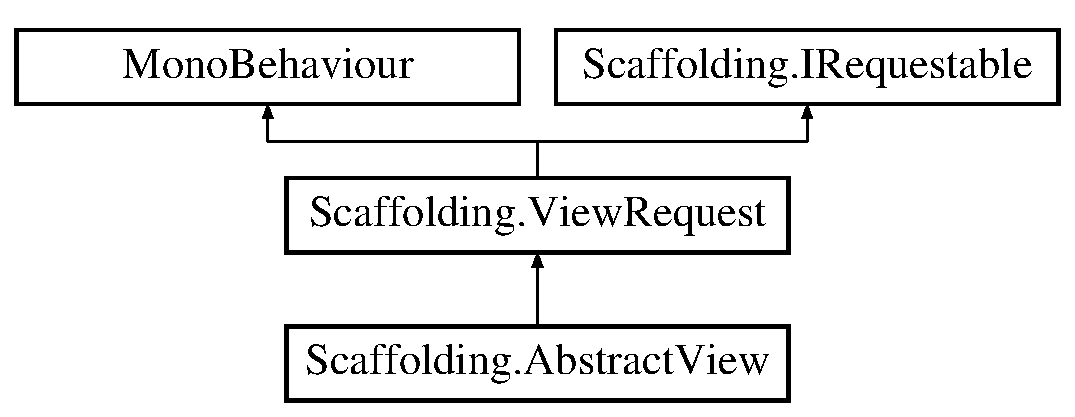
\includegraphics[height=3.000000cm]{class_scaffolding_1_1_view_request}
\end{center}
\end{figure}
\subsection*{Public Member Functions}
\begin{DoxyCompactItemize}
\item 
\hypertarget{class_scaffolding_1_1_view_request_afa476fd65d761a75a17763aa66ec4526}{virtual void {\bfseries Register\+View\+To\+Model} (\hyperlink{class_scaffolding_1_1_abstract_view}{Abstract\+View} view, \hyperlink{class_scaffolding_1_1_abstract_model}{Abstract\+Model} model)}\label{class_scaffolding_1_1_view_request_afa476fd65d761a75a17763aa66ec4526}

\item 
\hyperlink{class_scaffolding_1_1_s_object}{S\+Object} \hyperlink{class_scaffolding_1_1_view_request_a3edc966ebf54c7695dd2918007d5f433}{Get\+View\+Data\+For\+Transition} (Type type)
\begin{DoxyCompactList}\small\item\em Get the data that has been packaged for delivery to a view. \end{DoxyCompactList}\item 
virtual void \hyperlink{class_scaffolding_1_1_view_request_aa673715af6dd0fe2faa4d825d13a734d}{Request\+Overlay$<$ T $>$} ()
\begin{DoxyCompactList}\small\item\em Requests an overlay to open. \end{DoxyCompactList}\item 
virtual void \hyperlink{class_scaffolding_1_1_view_request_a73035af50a3c6e23e5de1798df478911}{Request\+Overlay} (Type type)
\begin{DoxyCompactList}\small\item\em Request an overlay with type to open. \end{DoxyCompactList}\item 
virtual void \hyperlink{class_scaffolding_1_1_view_request_a3eddf134fb24bde36070703528f48688}{Request\+Overlay$<$ T $>$} (bool disable\+Inputs\+On\+Screen)
\begin{DoxyCompactList}\small\item\em Requests an overlay to open, with the option to disable inputs on the currently open screen \end{DoxyCompactList}\item 
virtual void \hyperlink{class_scaffolding_1_1_view_request_af2db772c0e32b01dd9576bfa24ce04aa}{Request\+Overlay} (Type type, bool disable\+Inputs\+On\+Screen)
\begin{DoxyCompactList}\small\item\em Requests an overlay to open, with the option to disable inputs on the currently open screen \end{DoxyCompactList}\item 
virtual void \hyperlink{class_scaffolding_1_1_view_request_a614cdfd9b456ef39d9294c4f0a5d4a4b}{Request\+Overlay\+Close$<$ T $>$} ()
\begin{DoxyCompactList}\small\item\em Request an overlay to close. \end{DoxyCompactList}\item 
virtual void \hyperlink{class_scaffolding_1_1_view_request_a8e2b65d409c7b4ff692753ce5825e9de}{Request\+Overlay\+Close} (Type type)
\begin{DoxyCompactList}\small\item\em Request an overlay to close of type. \end{DoxyCompactList}\item 
virtual void \hyperlink{class_scaffolding_1_1_view_request_ad546a557c876f40350a0aa87e3df051f}{Request\+Overlay\+Force\+Close$<$ T $>$} ()
\begin{DoxyCompactList}\small\item\em Force an overlay to close, this skips the On\+Hide\+Start method and goes straight to Hide\+Complete. \end{DoxyCompactList}\item 
virtual void \hyperlink{class_scaffolding_1_1_view_request_a9245c7504ef075c0a800b1d63db3a7c4}{Request\+Overlay\+Force\+Close} (Type type)
\begin{DoxyCompactList}\small\item\em Force an overlay to close, this skips the On\+Hide\+Start method and goes straight to Hide\+Complete. \end{DoxyCompactList}\item 
virtual void \hyperlink{class_scaffolding_1_1_view_request_acacc176c1e97491d4ed539b71a0576c8}{Request\+View$<$ T $>$} ()
\begin{DoxyCompactList}\small\item\em Request a view. \end{DoxyCompactList}\item 
virtual void \hyperlink{class_scaffolding_1_1_view_request_a6049ec6f948d31b1f38252f8c330aa34}{Request\+View} (Type type)
\begin{DoxyCompactList}\small\item\em Request a view with type. \end{DoxyCompactList}\item 
virtual void \hyperlink{class_scaffolding_1_1_view_request_a5c031132968ce946ce612ca3a79b1075}{Request\+Force\+Reopen\+View$<$ T $>$} ()
\begin{DoxyCompactList}\small\item\em Request to reopen a view \end{DoxyCompactList}\item 
virtual void \hyperlink{class_scaffolding_1_1_view_request_af867121a024ce722629fe9ad23a8207f}{Request\+Force\+Reopen\+View} (Type type)
\begin{DoxyCompactList}\small\item\em Request to reopen a view \end{DoxyCompactList}\item 
virtual void \hyperlink{class_scaffolding_1_1_view_request_ae9834b37d6a291e9666f1d47a0614e74}{Request\+View\+With\+Loading\+Overlay$<$ T, L $>$} ()
\begin{DoxyCompactList}\small\item\em Request a view, with an overlay. Used when the requested view is a heavy load and you want to mask that stall with a loading screen. \end{DoxyCompactList}\item 
virtual void \hyperlink{class_scaffolding_1_1_view_request_a46ea4104f8158757661c1626b074b665}{Request\+View\+With\+Loading\+Overlay} (Type type, Type loading\+Type)
\begin{DoxyCompactList}\small\item\em Request a view, with an overlay. Used when the requested view is a heavy load and you want to mask that stall with a loading screen. \end{DoxyCompactList}\item 
void \hyperlink{class_scaffolding_1_1_view_request_af8aa731570962d7a79a83575726e033e}{Send\+Data\+To\+View$<$ T $>$} (\hyperlink{class_scaffolding_1_1_s_object}{S\+Object} data)
\begin{DoxyCompactList}\small\item\em Package up data to send to a target view. Useful to send data between views, can be packaged anytime before the change view request happens. \end{DoxyCompactList}\item 
void \hyperlink{class_scaffolding_1_1_view_request_a9ed5d8133e13eeb40abf1c897e89401d}{Send\+Data\+To\+View} (Type target\+View, \hyperlink{class_scaffolding_1_1_s_object}{S\+Object} data)
\begin{DoxyCompactList}\small\item\em Package up data to send to a target view. Useful to send data between views, can be packaged anytime before the change view request happens. \end{DoxyCompactList}\item 
void \hyperlink{class_scaffolding_1_1_view_request_a352884d93e18dbe65225c4c0f0a2a291}{Remove\+Data\+For\+View$<$ T $>$} ()
\begin{DoxyCompactList}\small\item\em Delete any data you want to send to a view. \end{DoxyCompactList}\item 
void \hyperlink{class_scaffolding_1_1_view_request_a74c5d71a0743934fba7f6980e7decd7a}{Remove\+Data\+For\+View} (Type target\+View)
\begin{DoxyCompactList}\small\item\em Delete any data you want to send to a view. \end{DoxyCompactList}\end{DoxyCompactItemize}
\subsection*{Properties}
\begin{DoxyCompactItemize}
\item 
bool \hyperlink{class_scaffolding_1_1_view_request_ae88834823495c1f661407d885e3c5e9d}{Is\+Hiding}\hspace{0.3cm}{\ttfamily  \mbox{[}get\mbox{]}}
\begin{DoxyCompactList}\small\item\em Gets a value indicating whether or not this view is in the hide state. \end{DoxyCompactList}\item 
bool \hyperlink{class_scaffolding_1_1_view_request_a56767533f14295a74852fdb2f855504f}{Is\+Showing}\hspace{0.3cm}{\ttfamily  \mbox{[}get\mbox{]}}
\begin{DoxyCompactList}\small\item\em Gets a value indicating whether or not this view is in the showing state. \end{DoxyCompactList}\item 
\hypertarget{class_scaffolding_1_1_view_request_af715820a9f7d30c529a29013fce1100c}{bool {\bfseries Is\+Setting\+Up}\hspace{0.3cm}{\ttfamily  \mbox{[}get\mbox{]}}}\label{class_scaffolding_1_1_view_request_af715820a9f7d30c529a29013fce1100c}

\end{DoxyCompactItemize}


\subsection{Member Function Documentation}
\hypertarget{class_scaffolding_1_1_view_request_a3edc966ebf54c7695dd2918007d5f433}{\index{Scaffolding\+::\+View\+Request@{Scaffolding\+::\+View\+Request}!Get\+View\+Data\+For\+Transition@{Get\+View\+Data\+For\+Transition}}
\index{Get\+View\+Data\+For\+Transition@{Get\+View\+Data\+For\+Transition}!Scaffolding\+::\+View\+Request@{Scaffolding\+::\+View\+Request}}
\subsubsection[{Get\+View\+Data\+For\+Transition}]{\setlength{\rightskip}{0pt plus 5cm}{\bf S\+Object} Scaffolding.\+View\+Request.\+Get\+View\+Data\+For\+Transition (
\begin{DoxyParamCaption}
\item[{Type}]{type}
\end{DoxyParamCaption}
)}}\label{class_scaffolding_1_1_view_request_a3edc966ebf54c7695dd2918007d5f433}


Get the data that has been packaged for delivery to a view. 

\hypertarget{class_scaffolding_1_1_view_request_a74c5d71a0743934fba7f6980e7decd7a}{\index{Scaffolding\+::\+View\+Request@{Scaffolding\+::\+View\+Request}!Remove\+Data\+For\+View@{Remove\+Data\+For\+View}}
\index{Remove\+Data\+For\+View@{Remove\+Data\+For\+View}!Scaffolding\+::\+View\+Request@{Scaffolding\+::\+View\+Request}}
\subsubsection[{Remove\+Data\+For\+View}]{\setlength{\rightskip}{0pt plus 5cm}void Scaffolding.\+View\+Request.\+Remove\+Data\+For\+View (
\begin{DoxyParamCaption}
\item[{Type}]{target\+View}
\end{DoxyParamCaption}
)}}\label{class_scaffolding_1_1_view_request_a74c5d71a0743934fba7f6980e7decd7a}


Delete any data you want to send to a view. 


\begin{DoxyParams}{Parameters}
{\em target\+View} & Target view.\\
\hline
\end{DoxyParams}
\hypertarget{class_scaffolding_1_1_view_request_a352884d93e18dbe65225c4c0f0a2a291}{\index{Scaffolding\+::\+View\+Request@{Scaffolding\+::\+View\+Request}!Remove\+Data\+For\+View$<$ T $>$@{Remove\+Data\+For\+View$<$ T $>$}}
\index{Remove\+Data\+For\+View$<$ T $>$@{Remove\+Data\+For\+View$<$ T $>$}!Scaffolding\+::\+View\+Request@{Scaffolding\+::\+View\+Request}}
\subsubsection[{Remove\+Data\+For\+View$<$ T $>$}]{\setlength{\rightskip}{0pt plus 5cm}void {\bf Scaffolding.\+View\+Request.\+Remove\+Data\+For\+View}$<$ T $>$ (
\begin{DoxyParamCaption}
{}
\end{DoxyParamCaption}
)}}\label{class_scaffolding_1_1_view_request_a352884d93e18dbe65225c4c0f0a2a291}


Delete any data you want to send to a view. 


\begin{DoxyParams}{Parameters}
{\em target\+View} & Target view.\\
\hline
\end{DoxyParams}
\begin{Desc}
\item[Type Constraints]\begin{description}
\item[{\em T} : {\em Abstract\+View}]\end{description}
\end{Desc}
\hypertarget{class_scaffolding_1_1_view_request_af867121a024ce722629fe9ad23a8207f}{\index{Scaffolding\+::\+View\+Request@{Scaffolding\+::\+View\+Request}!Request\+Force\+Reopen\+View@{Request\+Force\+Reopen\+View}}
\index{Request\+Force\+Reopen\+View@{Request\+Force\+Reopen\+View}!Scaffolding\+::\+View\+Request@{Scaffolding\+::\+View\+Request}}
\subsubsection[{Request\+Force\+Reopen\+View}]{\setlength{\rightskip}{0pt plus 5cm}virtual void Scaffolding.\+View\+Request.\+Request\+Force\+Reopen\+View (
\begin{DoxyParamCaption}
\item[{Type}]{type}
\end{DoxyParamCaption}
)\hspace{0.3cm}{\ttfamily [virtual]}}}\label{class_scaffolding_1_1_view_request_af867121a024ce722629fe9ad23a8207f}


Request to reopen a view 


\begin{DoxyParams}{Parameters}
{\em type} & Type.\\
\hline
\end{DoxyParams}


Implements \hyperlink{interface_scaffolding_1_1_i_requestable}{Scaffolding.\+I\+Requestable}.

\hypertarget{class_scaffolding_1_1_view_request_a5c031132968ce946ce612ca3a79b1075}{\index{Scaffolding\+::\+View\+Request@{Scaffolding\+::\+View\+Request}!Request\+Force\+Reopen\+View$<$ T $>$@{Request\+Force\+Reopen\+View$<$ T $>$}}
\index{Request\+Force\+Reopen\+View$<$ T $>$@{Request\+Force\+Reopen\+View$<$ T $>$}!Scaffolding\+::\+View\+Request@{Scaffolding\+::\+View\+Request}}
\subsubsection[{Request\+Force\+Reopen\+View$<$ T $>$}]{\setlength{\rightskip}{0pt plus 5cm}virtual void {\bf Scaffolding.\+View\+Request.\+Request\+Force\+Reopen\+View}$<$ T $>$ (
\begin{DoxyParamCaption}
{}
\end{DoxyParamCaption}
)\hspace{0.3cm}{\ttfamily [virtual]}}}\label{class_scaffolding_1_1_view_request_a5c031132968ce946ce612ca3a79b1075}


Request to reopen a view 


\begin{DoxyTemplParams}{Template Parameters}
{\em T} & The 1st type parameter.\\
\hline
\end{DoxyTemplParams}


Implements \hyperlink{interface_scaffolding_1_1_i_requestable}{Scaffolding.\+I\+Requestable}.

\begin{Desc}
\item[Type Constraints]\begin{description}
\item[{\em T} : {\em Abstract\+View}]\end{description}
\end{Desc}
\hypertarget{class_scaffolding_1_1_view_request_a73035af50a3c6e23e5de1798df478911}{\index{Scaffolding\+::\+View\+Request@{Scaffolding\+::\+View\+Request}!Request\+Overlay@{Request\+Overlay}}
\index{Request\+Overlay@{Request\+Overlay}!Scaffolding\+::\+View\+Request@{Scaffolding\+::\+View\+Request}}
\subsubsection[{Request\+Overlay}]{\setlength{\rightskip}{0pt plus 5cm}virtual void Scaffolding.\+View\+Request.\+Request\+Overlay (
\begin{DoxyParamCaption}
\item[{Type}]{type}
\end{DoxyParamCaption}
)\hspace{0.3cm}{\ttfamily [virtual]}}}\label{class_scaffolding_1_1_view_request_a73035af50a3c6e23e5de1798df478911}


Request an overlay with type to open. 

Example\+: Request\+Overlay(typeof(\+My\+View)); 

Implements \hyperlink{interface_scaffolding_1_1_i_requestable}{Scaffolding.\+I\+Requestable}.

\hypertarget{class_scaffolding_1_1_view_request_af2db772c0e32b01dd9576bfa24ce04aa}{\index{Scaffolding\+::\+View\+Request@{Scaffolding\+::\+View\+Request}!Request\+Overlay@{Request\+Overlay}}
\index{Request\+Overlay@{Request\+Overlay}!Scaffolding\+::\+View\+Request@{Scaffolding\+::\+View\+Request}}
\subsubsection[{Request\+Overlay}]{\setlength{\rightskip}{0pt plus 5cm}virtual void Scaffolding.\+View\+Request.\+Request\+Overlay (
\begin{DoxyParamCaption}
\item[{Type}]{type, }
\item[{bool}]{disable\+Inputs\+On\+Screen}
\end{DoxyParamCaption}
)\hspace{0.3cm}{\ttfamily [virtual]}}}\label{class_scaffolding_1_1_view_request_af2db772c0e32b01dd9576bfa24ce04aa}


Requests an overlay to open, with the option to disable inputs on the currently open screen 


\begin{DoxyParams}{Parameters}
{\em type} & Type.\\
\hline
{\em disable\+Inputs\+On\+Screen} & If set to {\ttfamily true} disable inputs on screen.\\
\hline
\end{DoxyParams}
\hypertarget{class_scaffolding_1_1_view_request_aa673715af6dd0fe2faa4d825d13a734d}{\index{Scaffolding\+::\+View\+Request@{Scaffolding\+::\+View\+Request}!Request\+Overlay$<$ T $>$@{Request\+Overlay$<$ T $>$}}
\index{Request\+Overlay$<$ T $>$@{Request\+Overlay$<$ T $>$}!Scaffolding\+::\+View\+Request@{Scaffolding\+::\+View\+Request}}
\subsubsection[{Request\+Overlay$<$ T $>$}]{\setlength{\rightskip}{0pt plus 5cm}virtual void {\bf Scaffolding.\+View\+Request.\+Request\+Overlay}$<$ T $>$ (
\begin{DoxyParamCaption}
{}
\end{DoxyParamCaption}
)\hspace{0.3cm}{\ttfamily [virtual]}}}\label{class_scaffolding_1_1_view_request_aa673715af6dd0fe2faa4d825d13a734d}


Requests an overlay to open. 

Example\+: \hyperlink{class_scaffolding_1_1_view_request_a73035af50a3c6e23e5de1798df478911}{Request\+Overlay$<$\+My\+View$>$()}; 


\begin{DoxyTemplParams}{Template Parameters}
{\em T} & The 1st type parameter.\\
\hline
\end{DoxyTemplParams}


Implements \hyperlink{interface_scaffolding_1_1_i_requestable}{Scaffolding.\+I\+Requestable}.

\begin{Desc}
\item[Type Constraints]\begin{description}
\item[{\em T} : {\em Abstract\+View}]\end{description}
\end{Desc}
\hypertarget{class_scaffolding_1_1_view_request_a3eddf134fb24bde36070703528f48688}{\index{Scaffolding\+::\+View\+Request@{Scaffolding\+::\+View\+Request}!Request\+Overlay$<$ T $>$@{Request\+Overlay$<$ T $>$}}
\index{Request\+Overlay$<$ T $>$@{Request\+Overlay$<$ T $>$}!Scaffolding\+::\+View\+Request@{Scaffolding\+::\+View\+Request}}
\subsubsection[{Request\+Overlay$<$ T $>$}]{\setlength{\rightskip}{0pt plus 5cm}virtual void {\bf Scaffolding.\+View\+Request.\+Request\+Overlay}$<$ T $>$ (
\begin{DoxyParamCaption}
\item[{bool}]{disable\+Inputs\+On\+Screen}
\end{DoxyParamCaption}
)\hspace{0.3cm}{\ttfamily [virtual]}}}\label{class_scaffolding_1_1_view_request_a3eddf134fb24bde36070703528f48688}


Requests an overlay to open, with the option to disable inputs on the currently open screen 


\begin{DoxyParams}{Parameters}
{\em disable\+Inputs\+On\+Screen} & If set to {\ttfamily true} disable inputs on screen.\\
\hline
\end{DoxyParams}

\begin{DoxyTemplParams}{Template Parameters}
{\em T} & The 1st type parameter.\\
\hline
\end{DoxyTemplParams}
\hypertarget{class_scaffolding_1_1_view_request_a8e2b65d409c7b4ff692753ce5825e9de}{\index{Scaffolding\+::\+View\+Request@{Scaffolding\+::\+View\+Request}!Request\+Overlay\+Close@{Request\+Overlay\+Close}}
\index{Request\+Overlay\+Close@{Request\+Overlay\+Close}!Scaffolding\+::\+View\+Request@{Scaffolding\+::\+View\+Request}}
\subsubsection[{Request\+Overlay\+Close}]{\setlength{\rightskip}{0pt plus 5cm}virtual void Scaffolding.\+View\+Request.\+Request\+Overlay\+Close (
\begin{DoxyParamCaption}
\item[{Type}]{type}
\end{DoxyParamCaption}
)\hspace{0.3cm}{\ttfamily [virtual]}}}\label{class_scaffolding_1_1_view_request_a8e2b65d409c7b4ff692753ce5825e9de}


Request an overlay to close of type. 

Example\+: Request\+Overlay\+Close(typeof(\+My\+View)); 

Implements \hyperlink{interface_scaffolding_1_1_i_requestable}{Scaffolding.\+I\+Requestable}.

\hypertarget{class_scaffolding_1_1_view_request_a614cdfd9b456ef39d9294c4f0a5d4a4b}{\index{Scaffolding\+::\+View\+Request@{Scaffolding\+::\+View\+Request}!Request\+Overlay\+Close$<$ T $>$@{Request\+Overlay\+Close$<$ T $>$}}
\index{Request\+Overlay\+Close$<$ T $>$@{Request\+Overlay\+Close$<$ T $>$}!Scaffolding\+::\+View\+Request@{Scaffolding\+::\+View\+Request}}
\subsubsection[{Request\+Overlay\+Close$<$ T $>$}]{\setlength{\rightskip}{0pt plus 5cm}virtual void {\bf Scaffolding.\+View\+Request.\+Request\+Overlay\+Close}$<$ T $>$ (
\begin{DoxyParamCaption}
{}
\end{DoxyParamCaption}
)\hspace{0.3cm}{\ttfamily [virtual]}}}\label{class_scaffolding_1_1_view_request_a614cdfd9b456ef39d9294c4f0a5d4a4b}


Request an overlay to close. 

Example\+: \hyperlink{class_scaffolding_1_1_view_request_a8e2b65d409c7b4ff692753ce5825e9de}{Request\+Overlay\+Close$<$\+My\+View$>$()}; 

Implements \hyperlink{interface_scaffolding_1_1_i_requestable}{Scaffolding.\+I\+Requestable}.

\begin{Desc}
\item[Type Constraints]\begin{description}
\item[{\em T} : {\em Abstract\+View}]\end{description}
\end{Desc}
\hypertarget{class_scaffolding_1_1_view_request_a9245c7504ef075c0a800b1d63db3a7c4}{\index{Scaffolding\+::\+View\+Request@{Scaffolding\+::\+View\+Request}!Request\+Overlay\+Force\+Close@{Request\+Overlay\+Force\+Close}}
\index{Request\+Overlay\+Force\+Close@{Request\+Overlay\+Force\+Close}!Scaffolding\+::\+View\+Request@{Scaffolding\+::\+View\+Request}}
\subsubsection[{Request\+Overlay\+Force\+Close}]{\setlength{\rightskip}{0pt plus 5cm}virtual void Scaffolding.\+View\+Request.\+Request\+Overlay\+Force\+Close (
\begin{DoxyParamCaption}
\item[{Type}]{type}
\end{DoxyParamCaption}
)\hspace{0.3cm}{\ttfamily [virtual]}}}\label{class_scaffolding_1_1_view_request_a9245c7504ef075c0a800b1d63db3a7c4}


Force an overlay to close, this skips the On\+Hide\+Start method and goes straight to Hide\+Complete. 

Example\+: Request\+Overlay\+Force\+Close(typeof(\+My\+View)); 

Implements \hyperlink{interface_scaffolding_1_1_i_requestable}{Scaffolding.\+I\+Requestable}.

\hypertarget{class_scaffolding_1_1_view_request_ad546a557c876f40350a0aa87e3df051f}{\index{Scaffolding\+::\+View\+Request@{Scaffolding\+::\+View\+Request}!Request\+Overlay\+Force\+Close$<$ T $>$@{Request\+Overlay\+Force\+Close$<$ T $>$}}
\index{Request\+Overlay\+Force\+Close$<$ T $>$@{Request\+Overlay\+Force\+Close$<$ T $>$}!Scaffolding\+::\+View\+Request@{Scaffolding\+::\+View\+Request}}
\subsubsection[{Request\+Overlay\+Force\+Close$<$ T $>$}]{\setlength{\rightskip}{0pt plus 5cm}virtual void {\bf Scaffolding.\+View\+Request.\+Request\+Overlay\+Force\+Close}$<$ T $>$ (
\begin{DoxyParamCaption}
{}
\end{DoxyParamCaption}
)\hspace{0.3cm}{\ttfamily [virtual]}}}\label{class_scaffolding_1_1_view_request_ad546a557c876f40350a0aa87e3df051f}


Force an overlay to close, this skips the On\+Hide\+Start method and goes straight to Hide\+Complete. 

Example\+: \hyperlink{class_scaffolding_1_1_view_request_a9245c7504ef075c0a800b1d63db3a7c4}{Request\+Overlay\+Force\+Close$<$\+My\+View$>$()}; 

Implements \hyperlink{interface_scaffolding_1_1_i_requestable}{Scaffolding.\+I\+Requestable}.

\begin{Desc}
\item[Type Constraints]\begin{description}
\item[{\em T} : {\em Abstract\+View}]\end{description}
\end{Desc}
\hypertarget{class_scaffolding_1_1_view_request_a6049ec6f948d31b1f38252f8c330aa34}{\index{Scaffolding\+::\+View\+Request@{Scaffolding\+::\+View\+Request}!Request\+View@{Request\+View}}
\index{Request\+View@{Request\+View}!Scaffolding\+::\+View\+Request@{Scaffolding\+::\+View\+Request}}
\subsubsection[{Request\+View}]{\setlength{\rightskip}{0pt plus 5cm}virtual void Scaffolding.\+View\+Request.\+Request\+View (
\begin{DoxyParamCaption}
\item[{Type}]{type}
\end{DoxyParamCaption}
)\hspace{0.3cm}{\ttfamily [virtual]}}}\label{class_scaffolding_1_1_view_request_a6049ec6f948d31b1f38252f8c330aa34}


Request a view with type. 

Example\+: Request\+View(typeof(\+My\+View)); 

Implements \hyperlink{interface_scaffolding_1_1_i_requestable}{Scaffolding.\+I\+Requestable}.

\hypertarget{class_scaffolding_1_1_view_request_acacc176c1e97491d4ed539b71a0576c8}{\index{Scaffolding\+::\+View\+Request@{Scaffolding\+::\+View\+Request}!Request\+View$<$ T $>$@{Request\+View$<$ T $>$}}
\index{Request\+View$<$ T $>$@{Request\+View$<$ T $>$}!Scaffolding\+::\+View\+Request@{Scaffolding\+::\+View\+Request}}
\subsubsection[{Request\+View$<$ T $>$}]{\setlength{\rightskip}{0pt plus 5cm}virtual void {\bf Scaffolding.\+View\+Request.\+Request\+View}$<$ T $>$ (
\begin{DoxyParamCaption}
{}
\end{DoxyParamCaption}
)\hspace{0.3cm}{\ttfamily [virtual]}}}\label{class_scaffolding_1_1_view_request_acacc176c1e97491d4ed539b71a0576c8}


Request a view. 

Example\+: \hyperlink{class_scaffolding_1_1_view_request_a6049ec6f948d31b1f38252f8c330aa34}{Request\+View$<$\+My\+View$>$()}; 

Implements \hyperlink{interface_scaffolding_1_1_i_requestable}{Scaffolding.\+I\+Requestable}.

\begin{Desc}
\item[Type Constraints]\begin{description}
\item[{\em T} : {\em Abstract\+View}]\end{description}
\end{Desc}
\hypertarget{class_scaffolding_1_1_view_request_a46ea4104f8158757661c1626b074b665}{\index{Scaffolding\+::\+View\+Request@{Scaffolding\+::\+View\+Request}!Request\+View\+With\+Loading\+Overlay@{Request\+View\+With\+Loading\+Overlay}}
\index{Request\+View\+With\+Loading\+Overlay@{Request\+View\+With\+Loading\+Overlay}!Scaffolding\+::\+View\+Request@{Scaffolding\+::\+View\+Request}}
\subsubsection[{Request\+View\+With\+Loading\+Overlay}]{\setlength{\rightskip}{0pt plus 5cm}virtual void Scaffolding.\+View\+Request.\+Request\+View\+With\+Loading\+Overlay (
\begin{DoxyParamCaption}
\item[{Type}]{type, }
\item[{Type}]{loading\+Type}
\end{DoxyParamCaption}
)\hspace{0.3cm}{\ttfamily [virtual]}}}\label{class_scaffolding_1_1_view_request_a46ea4104f8158757661c1626b074b665}


Request a view, with an overlay. Used when the requested view is a heavy load and you want to mask that stall with a loading screen. 

Example\+: Request\+View\+With\+Loading\+Overlay(typeof(\+My\+Heavy\+View),typeof(\+My\+Loading\+Screen)); 

Implements \hyperlink{interface_scaffolding_1_1_i_requestable}{Scaffolding.\+I\+Requestable}.

\hypertarget{class_scaffolding_1_1_view_request_ae9834b37d6a291e9666f1d47a0614e74}{\index{Scaffolding\+::\+View\+Request@{Scaffolding\+::\+View\+Request}!Request\+View\+With\+Loading\+Overlay$<$ T, L $>$@{Request\+View\+With\+Loading\+Overlay$<$ T, L $>$}}
\index{Request\+View\+With\+Loading\+Overlay$<$ T, L $>$@{Request\+View\+With\+Loading\+Overlay$<$ T, L $>$}!Scaffolding\+::\+View\+Request@{Scaffolding\+::\+View\+Request}}
\subsubsection[{Request\+View\+With\+Loading\+Overlay$<$ T, L $>$}]{\setlength{\rightskip}{0pt plus 5cm}virtual void {\bf Scaffolding.\+View\+Request.\+Request\+View\+With\+Loading\+Overlay}$<$ T, L $>$ (
\begin{DoxyParamCaption}
{}
\end{DoxyParamCaption}
)\hspace{0.3cm}{\ttfamily [virtual]}}}\label{class_scaffolding_1_1_view_request_ae9834b37d6a291e9666f1d47a0614e74}


Request a view, with an overlay. Used when the requested view is a heavy load and you want to mask that stall with a loading screen. 

Example\+: \hyperlink{class_scaffolding_1_1_view_request_a46ea4104f8158757661c1626b074b665}{Request\+View\+With\+Loading\+Overlay$<$\+My\+Heavy\+View, My\+Loading\+Screen$>$()}; 

Implements \hyperlink{interface_scaffolding_1_1_i_requestable}{Scaffolding.\+I\+Requestable}.

\begin{Desc}
\item[Type Constraints]\begin{description}
\item[{\em T} : {\em Abstract\+View}]\item[{\em L} : {\em Abstract\+View}]\end{description}
\end{Desc}
\hypertarget{class_scaffolding_1_1_view_request_a9ed5d8133e13eeb40abf1c897e89401d}{\index{Scaffolding\+::\+View\+Request@{Scaffolding\+::\+View\+Request}!Send\+Data\+To\+View@{Send\+Data\+To\+View}}
\index{Send\+Data\+To\+View@{Send\+Data\+To\+View}!Scaffolding\+::\+View\+Request@{Scaffolding\+::\+View\+Request}}
\subsubsection[{Send\+Data\+To\+View}]{\setlength{\rightskip}{0pt plus 5cm}void Scaffolding.\+View\+Request.\+Send\+Data\+To\+View (
\begin{DoxyParamCaption}
\item[{Type}]{target\+View, }
\item[{{\bf S\+Object}}]{data}
\end{DoxyParamCaption}
)}}\label{class_scaffolding_1_1_view_request_a9ed5d8133e13eeb40abf1c897e89401d}


Package up data to send to a target view. Useful to send data between views, can be packaged anytime before the change view request happens. 

Example\+: Value\+Object obj = new Value\+Object(); obj.\+Put\+Int(\char`\"{}\+Key\char`\"{}, 10); Send\+Data\+To\+View(type\+Of(\+My\+View),obj); \hypertarget{class_scaffolding_1_1_view_request_af8aa731570962d7a79a83575726e033e}{\index{Scaffolding\+::\+View\+Request@{Scaffolding\+::\+View\+Request}!Send\+Data\+To\+View$<$ T $>$@{Send\+Data\+To\+View$<$ T $>$}}
\index{Send\+Data\+To\+View$<$ T $>$@{Send\+Data\+To\+View$<$ T $>$}!Scaffolding\+::\+View\+Request@{Scaffolding\+::\+View\+Request}}
\subsubsection[{Send\+Data\+To\+View$<$ T $>$}]{\setlength{\rightskip}{0pt plus 5cm}void {\bf Scaffolding.\+View\+Request.\+Send\+Data\+To\+View}$<$ T $>$ (
\begin{DoxyParamCaption}
\item[{{\bf S\+Object}}]{data}
\end{DoxyParamCaption}
)}}\label{class_scaffolding_1_1_view_request_af8aa731570962d7a79a83575726e033e}


Package up data to send to a target view. Useful to send data between views, can be packaged anytime before the change view request happens. 

Example\+: Value\+Object obj = new Value\+Object(); obj.\+Put\+Int(\char`\"{}\+Key\char`\"{}, 10); Send\+Data\+To\+View$<$\+My\+View$>$(obj); \begin{Desc}
\item[Type Constraints]\begin{description}
\item[{\em T} : {\em Abstract\+View}]\end{description}
\end{Desc}


\subsection{Property Documentation}
\hypertarget{class_scaffolding_1_1_view_request_ae88834823495c1f661407d885e3c5e9d}{\index{Scaffolding\+::\+View\+Request@{Scaffolding\+::\+View\+Request}!Is\+Hiding@{Is\+Hiding}}
\index{Is\+Hiding@{Is\+Hiding}!Scaffolding\+::\+View\+Request@{Scaffolding\+::\+View\+Request}}
\subsubsection[{Is\+Hiding}]{\setlength{\rightskip}{0pt plus 5cm}bool Scaffolding.\+View\+Request.\+Is\+Hiding\hspace{0.3cm}{\ttfamily [get]}}}\label{class_scaffolding_1_1_view_request_ae88834823495c1f661407d885e3c5e9d}


Gets a value indicating whether or not this view is in the hide state. 

{\ttfamily true} if this instance is hiding; otherwise, {\ttfamily false}.\hypertarget{class_scaffolding_1_1_view_request_a56767533f14295a74852fdb2f855504f}{\index{Scaffolding\+::\+View\+Request@{Scaffolding\+::\+View\+Request}!Is\+Showing@{Is\+Showing}}
\index{Is\+Showing@{Is\+Showing}!Scaffolding\+::\+View\+Request@{Scaffolding\+::\+View\+Request}}
\subsubsection[{Is\+Showing}]{\setlength{\rightskip}{0pt plus 5cm}bool Scaffolding.\+View\+Request.\+Is\+Showing\hspace{0.3cm}{\ttfamily [get]}}}\label{class_scaffolding_1_1_view_request_a56767533f14295a74852fdb2f855504f}


Gets a value indicating whether or not this view is in the showing state. 

{\ttfamily true} if this instance is showing; otherwise, {\ttfamily false}.

The documentation for this class was generated from the following file\+:\begin{DoxyCompactItemize}
\item 
Views/View\+Request.\+cs\end{DoxyCompactItemize}

%--- End generated contents ---

% Index
\newpage
\phantomsection
\addcontentsline{toc}{chapter}{Index}
\printindex

\end{document}
